%Tesi triennale
%Tommaso Boschi

%preamble
\documentclass[a4paper, usenatbib, 11pt]{book}
\usepackage[T1]{fontenc}
\usepackage[utf8]{inputenc}
\usepackage[italian, english]{babel}
\usepackage[hidelinks]{hyperref}
\usepackage{fancyhdr}
\usepackage{natbib}
\usepackage{indentfirst}
\usepackage{graphicx, import}
\usepackage{wrapfig}
%\usepackage{layaureo}
\usepackage[a4paper, total={6in, 8in}]{geometry}
\geometry{a4paper, total={150mm, 247mm}, left=30mm, top=30mm,}
\usepackage{pdfpages}
\usepackage{amssymb}
\usepackage{amsmath}
\usepackage{caption}
\usepackage{booktabs}
\usepackage{listings}
\usepackage{graphicx}
\usepackage{siunitx}
\sisetup{output-decimal-marker={.}}
\usepackage{color}
\usepackage{caption}
\usepackage{subfig}
\usepackage{threeparttable}
\usepackage{varwidth}
\usepackage{tikz}
\usepackage{multirow}
\usepackage{epstopdf}
\usepackage[autolanguage, np]{numprint}
\npfourdigitnosep
\usepackage{feynmp-auto}
%\usepackage{minipage}
%\usetikzlibrary{patterns}
%\usetikzlibrary{plotmarks}
\captionsetup{tableposition=top,figureposition=bottom,font=footnotesize}
\captionsetup{format=hang,labelfont={sf,bf}}
%\usepackage[backend=biber]{biblatex}

%\addbibresource{./one.bib}

\newcommand{\inch}{$^{\prime\prime}$}

\begin{document}

%Frontespissio
\includepdf[pages={1}]{myfronte.pdf}
\pagestyle{empty}

%Front
\frontmatter
\pagestyle{empty}
\begin{flushright}
  \emph{\large{Agli amici più grandi.}}

  \emph{\large{A chi ho perso per strada.}}
\end{flushright}


\clearpage
\pagestyle{plain}
\chapter{Overview}
This thesis is placed within the context of the %
The Accelerator Neutrino Neutron Interaction Experiment (ANNIE), a water Cherenkov %
detector built at the Fermi National Accelerator Laboratory.
The main aim of ANNIE is to study in depth the nature of neutrino-nucleus interactions %
by analysing the yield of final state neutrons produced in this kind of interactions.
New technologies, such as gadolinium-loaded water and, for the first time, %
Large Area Picosecond Photodetectors (LAPPDs) will be also employed in future phases of %
the experiment.
The measurement will have relevant implications for next generation Water Cherenkov detectors, %
in that these techniques may play a significant role %
in reducing backgrounds in relation to proton decay measurements, %
supernova neutrino observations and neutrino interaction physics.

This paper deals with the Phase I of the experiment, in which photomultipliers (PMT) are adopted %
within the tank and the forward Veto and the Muon Range Detector (MRD) are %
partially being employed.
A small container, called Neutron Volume Capture (NVC) %
is also inside the tank, for preliminary neutron yield studies.
%The MRD is a crucial component of the experiment in that it will help to tag signals properly.
The main work of the thesis consists of the development of the CAMAC electronics %
Data Acquisition system (DAQ); the already existing VME electronics DAQ, %
for the water PMTs, is also described.
Furthermore, early stage data are analysed and studied, and event reconstruction %
techniques are proposed.

All the described activities were undertaken in the Particle Physics Research Group of the %
Queen Mary University of London.

\vspace{25mm}
This thesis is divided as follows:
\begin{description}
  \item[Chapter~\ref{cha:1}] Neutrino Physics is briefly introducted and the experimental %
    techinques for their detection are listed.
  \item[Chapter~\ref{cha:2}] The ANNIE Experiment is descripted.
  \item[Chapter~\ref{cha:3}] The DAQ system is illustrated, as long as future developments.
  \item[Chapter~\ref{cha:4}] Data analysis techniques, mailny focused on signal/noise discrimination, %
    are shown. Event reconstruction is also taken in consideration.
  \item[Chapter~\ref{cha:5}] Measurements and testing the validy of preliminary data %
    analysis undertaken.
  \item[Chapter~\ref{cha:6}] Conclusion.
\end{description}


\tableofcontents

%Main
\mainmatter

\pagestyle{fancy}
\fancyfoot[LE,RO]{\thepage}
\renewcommand{\chaptermark}[1]{\markboth{\thechapter.\ #1}{}}
\fancyhf{}
\fancyhead[LE]{\scshape Phase I of the ANNIE experiment}
\fancyhead[RO]{\scshape \leftmark}
%\fancyheadoffset[LE,RO]{14pt}
\fancyfoot[CE,CO]{\thepage}

%%%%%%%%%%%%%%%%%%%%%%%%%%%%%%%		CHAP 1		%%%%%%%%%%%%%%%%%%%%%%%%%%%%%%%

\chapter{Introduction}
\label{cha:1}

 [From Giunti-Kim]
 The Standard Model (SM) is a gauge theory that describes the strong, electromagnetic, and weak interactions %
 of elementary particles in the framework of quantum field theory.
 The theory is based on the local symmetry group 
 \begin{equation}
   \label{eq:smgroup}
   \mathrm{SU(3)}_C \otimes \mathrm{SU(2)}_L \otimes \mathrm{U(1)}_Y
 \end{equation}
 where $C$, $L$ and $Y$ denote color, left-handed chirality and weak hypercharge, respectively.
 The gauge group uniquely determines the interactions and the number of %
 vector gauge bosons that correspond to the generators of the group.
 They are eight massless gluons that mediate strong interactions, %
 corresponding to the eight generators of SU(3)$_C$, and four gauge bosons, %
 of which three are massive ($W^\pm$ and $Z$) and one is massless, corresponding %
 to the three generators of SU(2)$_L$ and one generator of U(1)$_Y$, responsible for %
 electroweak interactions.
 The symmetry group of the SM fixes the interactions, i.e. the number and properties of the %
 vector gauge bosons, with only three independent unknown parameters: the three coupling constants of %
 the SU(3)$_C$, SU(2)$_L$, and U(1)$_Y$ groups, all of which must be determined from experiments.
 On the contrary, the number and properties of scalar bosons and fermions are left unconstrained, %
 except for the fact that they must transform according to the representations of the symmetry group, %
 while the fermion representations must lead to the cancellation of quantum anomalies.
 The known elementary fermions are divided in two categories, quarks and
 leptons, according to the scheme:
\begin{center}
  \small
  \begin{tabular}{lccc}
    \toprule
    \textbf{Generation}	&\textbf{1st}	& \textbf{2nd}	& \textbf{3rd}	\\
    \midrule
   \multirow{2}*{Quark} & $u$ 		& $c$		& $t$		\\
    			& $d$		& $s$		& $b$		\\
    \midrule
 \multirow{2}*{Letpons}	& $e$ 		& $\mu$		& $\tau$	\\
    			& $\nu_e$	& $\nu_\mu$	& $\nu_\tau$	\\
    \bottomrule
  \end{tabular}
\end{center}
 and their respective antiparticles.
 They are distinguished by the fact that quarks participate in all the interactions % 
 whereas leptons participate only in the electroweak interactions.

 In the SM, electroweak interactions can be studied separately from strong interactions, %
 because the symmetry under the color group is unbroken and there is no mixing %
 between the SU(3)$_C$ and the $\mathrm{SU(2)}_L \otimes \mathrm{U(1)}_Y$ sectors.
 On the other hand, the Glashow, Salam, and Weinberg theory well explains the group mixing between %
 electromagnetic and weak interactions caused by a symmetry breaking process.
 This model and the discovery of the predicted $W$ and $Z$ bosons, in addition to the gluon, %
 the top, and charm quarks, made the fortune of the Standard Model.
 Their redicted properties were experimentally confirmed with good precision and %
 the recent discovery of the Higgs Boson~\cite{atlas:higgs}~\cite{cms:higgs} %
 is the last crowning achievement of SM.

 Despite being the most successful theory of particle physics to date, the SM is actually limited %
 in its approximation to reality, in that some clear evidences cannot be explained.
 The most outstanding breakthrough is the neutrino oscillations, which was awarded the Nobel Prize in Physics in 2015 %
 and has proved that the neutrinos are not all massless, as it is assumed by theory.
 Mass terms for the neutrinos can be included in the SM, with the implications of theoretical problems.
 Likewise, the SM is unable to provide an explanation of the observed asymmetry between matter and anti-matter.
 It was noted by Sakharov that a solution to this puzzle would require some form of C and CP violation %
 in the early Universe, along with Baryon number violation and out-of-equilibrium interactions.
 These facts suggest that the Standard Model is not a complete theory and additional physics %
 Beyond the Standard Model (BSM) is required.
 
 The study of neutrinos is for sure one of the most promising probe to BSM physics and %
 is of vital importance to the future development of particle physics, %
 in particular through precision measurement of their interactions.
 A deep understanding of neutrino interactions, and neutrino-nucleon interactions in particular, %
 could lead to a great impact on long-baseline experiments, proton decay search, and supernova detection.

\section{Neutrino interactions}
 
 Neutrinos are colourless and chargless particles, thus sensitive only to weak interactions.
 Because of their nature, these leptons have small cross-sections and are difficult to measure.
 All the interactions are described by the the electroweak part of the SM, based on the symmetry group %
 $\mathrm{SU(2)}_L \otimes \mathrm{U(1)}_Y$, and are governed by the lagrangian %
 $\mathcal{L} = \mathcal{L}^{(CC)} + \mathcal{L}^{(NC)}$.
 In fact, neutrinos are mediated by the $W^\pm$ for charged-current (CC) interactions and by the $Z$ boson for %
 neutral-current (NC) ones, whose respective lagrangians are:
 \begin{align}
   \label{eq:cc}
   \mathcal{L}^{(CC)} &= - \frac{g}{2\sqrt{2}} \big (j^\mu_{W,L}W_\mu +\mathrm{h.c} \big ) \\
   \label{eq:nc}
   \mathcal{L}^{(NC)} &= - \frac{g}{2\cos\vartheta_{\mathrm{W}}} j^\mu_{Z,\nu}Z_\mu\,,
 \end{align}
 where the two currents are given by
 \begin{align}
   j^\mu_{W,L}   &= 2 \sum_{\alpha = e, \mu, \tau} \overline{\nu_{\alpha L}} \gamma^\mu l_{\alpha L} \\
   j^\mu_{Z,\nu}   & = \sum_{\alpha = e, \mu, \tau} \overline{\nu_{\alpha L}} \gamma^\mu \nu_{\alpha L}\,,
 \end{align}
 and $\vartheta_{\mathrm{W}} = \np{28.7}^\circ$ is the Weinberg angle.

 The easiest interaction that can be studied is the neutrino-electron elastic scattering
 \begin{equation}
   \nu_\alpha + e^- \rightarrow \nu_\alpha + e^-\,,
 \end{equation}
 and its antineutrino counterpart\footnote{In terms of Feynam diagrams, the \emph{t}-channel diagram is %
 replaced by the \emph{s}-channel diagram.}.
 For the electronic neutrino, both CC and NC interactions are allowed, while for $\alpha = \mu, \tau$ the %
 charged-current interactions are forbidden.
 The respective Feynman diagrams are shown in Fig.~\ref{fig:nescat} and~\ref{nutscat}.
 For low neutrino energies, where the effects of the $W$ and $Z$ propagators can be neglected, %
 the above processes are described by the effective charged-current and neutral-current lagrangians
 \begin{align}
   \mathcal{L}_\mathrm{eff}(\nu_e e^- \rightarrow \nu_e e^-) &= - \frac{G_F}{\sqrt{2}} %
   [\overline{\nu_e}\gamma^\mu(1-\gamma^5)\nu_e][\bar{e}\gamma_\mu((1+g_V^l)-(1+g_A^l)\gamma^5)e] \\
   \mathcal{L}_\mathrm{eff}(\nu_\alpha e^- \rightarrow \nu_\alpha e^-) &= - \frac{G_F}{\sqrt{2}} %
   [\overline{\nu_\alpha}\gamma^\mu(1-\gamma^5)\nu_\alpha][\bar{e}\gamma_\mu(g_V^l-g_A^l)\gamma^5)e] %
   \quad (\alpha = \mu,\tau)\,.
 \end{align}

 \begin{figure}
  \centering
 \begin{fmffile}{nescat}
   \begin{fmfgraph*}(100,80)
     \fmfleft{i2,i1}
     \fmfright{o2,o1}
     \fmf{fermion}{i1,v1,o1}
     \fmf{photon, label=$W$}{v1,v2}
     \fmf{fermion}{i2,v2,o2}
     \fmflabel{$\nu_e$}{i1}
     \fmflabel{$e^-$}{i2}
     \fmflabel{$e^-$}{o1}
     \fmflabel{$\nu_e$}{o2}
   \end{fmfgraph*}
   \quad + \quad
   \begin{fmfgraph*}(100,80)
     \fmfleft{i4,i3}
     \fmfright{o4,o3}
     \fmf{fermion}{i3,v3,o3}
     \fmf{photon, label=$Z$}{v3,v4}
     \fmf{fermion}{i4,v4,o4}
     \fmflabel{$\nu_e$}{i3}
     \fmflabel{$e^-$}{i4}
     \fmflabel{$\nu_e$}{o3}
     \fmflabel{$e^-$}{o4}
   \end{fmfgraph*}
 \end{fmffile}

 \captionsetup{skip=18pt}
 \caption{Tree-level Feynman diagrams for the process $\nu_e + e^- \rightarrow \nu_e + e^-$.
   The respective anti-neutrino CC interaction is a \emph{s}-channel process, instead.}
   \label{fig:nescat}
 \end{figure}

 \begin{figure}
  \centering
 \begin{fmffile}{nutscat}
   \begin{fmfgraph*}(100,80)
     \fmfleft{i2,i1}
     \fmfright{o2,o1}
     \fmf{fermion}{i1,v1,o1}
     \fmf{photon, label=$Z$}{v1,v2}
     \fmf{fermion}{i2,v2,o2}
     \fmflabel{$\nu_{\mu,\tau}$}{i1}
     \fmflabel{$e^-$}{i2}
     \fmflabel{$\nu_{\mu,\tau}$}{o1}
     \fmflabel{$e^-$}{o2}
   \end{fmfgraph*}
 \end{fmffile}

 \captionsetup{skip=18pt}
 \caption{Tree-level Feynman diagrams for the process $\nu_{\mu,\tau} + e^- \rightarrow \nu_{\mu,\tau} + e^-$.
   Only the NC process is permitted, which is also valid in the anit-neutrino case.}
   \label{fig:nutscat}
 \end{figure}

 The differential cross-section with respect to the momentum transfer $Q^2$
 \begin{equation}
   \frac{\mathrm{d}\sigma}{\mathrm{d}Q^2} = \frac{G_F^2}{\pi}\bigg[g_1^2 + g_2^2\bigg(1 - %
   \frac{Q^2}{2p_\nu \cdot p_e} \bigg)^2 - g_1 g_2 m_e^2 \frac{Q^2}{2 (p_\nu \cdot p_e)^2} \bigg]\,.
 \end{equation}
 The quantities $g_1$ and $g_2$ depend on the flavour of the neutrino and related to the vector and axial couplings, %
 $g_V$ and $g_A$.
 They are:
 \begin{align}
   g_1^{\nu_e} &= \frac{1}{2} + \sin^2\vartheta_W \quad , \quad
   g_2^{\nu_e} = \sin^2\vartheta_W \\
   g_1^{\nu_{\mu,\tau}} &= -\frac{1}{2} + \sin^2\vartheta_W \quad , \quad
   g_2^{\nu_{\mu,\tau}} = \sin^2\vartheta_W\,.
 \end{align}

 The differential cross-section as a function of the electron scattering angle in the laboratory frame is
 \begin{equation}
 \begin{split}
   \frac{\mathrm{d}\sigma}{\mathrm{d}\cos\theta} = \sigma_0 \frac{4 E_\nu^2 (m_e+E_\nu)^2 \cos \theta}%
   {\big[(m_e+E_\nu)^2-E_\nu^2 \cos^2 \theta \big]^2} \bigg[&g_1^2 + g_2^2\bigg(1 - %
   \frac{2 m_e E_\nu \cos^2 \theta}{(m_e+E_\nu)^2-E_\nu^2 \cos^2 \theta} \bigg)^2 \\
   - &g_1 g_2 \frac{2m_e^2 \cos^2 \theta}{(m_e+E_\nu)^2-E_\nu^2 \cos^2 \theta} \bigg]\,,
 \end{split}
 \end{equation}
 where 
 \begin{equation}
   \sigma_0 = \frac{2 G_F^2 m_e^2}{\pi}\,.
 \end{equation}

 For what concern the experiments, neutrino interactions with nucleons are easier to study thanks to the %
 much larger cross-section and a more diverse range of processes, despite being less straightforward to %
 deal with theoretically.
 In general, these processes can be categorised according to the momentum transfer.
 At small $Q^2$, elastic interactions dominate and may be brought about by both charged and neutral currents.
 When this occurs via neutral currents, all flavour of neutrinos and anti-neutrinos can scatter off %
 both neutrons and protons in what is referred to as ``NC elastic'' scattering.
 The process is:
 \begin{align}
   \nu_l + N \rightarrow \nu_l + N\,,
   \bar\nu_l + N \rightarrow \bar\nu_l + N\,,
 \end{align}

 Once neutrinos acquire sufficient energy they can also undergo the analogous charged current interactions, %
 called ``quasi-elastic'', due to the fact that the recoiling nucleon changes its charge and mass transfer occurs.
 The processes are
 \begin{align}
   \nu_l + n &\rightarrow p + l^-\,\\
   \bar\nu_l + p &\rightarrow n + l^+\,,
 \end{align}
 with $l=e, \mu, \tau$.
 For the muonic neutrino with energy below one GeV, the CCQE is the dominant interaction, event though the %
 cross-section plateaus at higher energies, as the available $Q^2$ increases: it becomes increasingly unlikely %
 for the nucleon to remain intact.

 The physics behind the CC quasi-elastic processes is more complicated.
 The differential cross-section for the scattering in the laboratory frame is given by
 \begin{equation}
   \label{eq:cc_xsec_q}
   \frac{\mathrm{d} \sigma_{CC}}{\mathrm{d}Q^2} = \frac{G_F^2 |V_{ud}|^2 m_N^4}{8\pi (p_\nu \cdot p_N)^2} %
   \bigg [A(Q^2) \pm B(Q^2) \frac{s-u}{m_N^2} + C(Q^2) \frac{(s-u)^2}{m_N^4} \bigg]\,,
 \end{equation}
 where the plus sign refers to the $N = n$ interactions, while the minus sign to $N = p$.

 \begin{equation}
   \label{eq:cc_xsec_t}
   \frac{\mathrm{d} \sigma_{CC}}{\mathrm{d}\cos\theta} = -\frac{G_F^2 |V_{ud}|^2 m_N^2}{4\pi} \frac{p_l}{E_\nu} %
   \bigg [A(Q^2) \pm B(Q^2) \frac{s-u}{m_N^2} + C(Q^2) \frac{(s-u)^2}{m_N^4} \bigg]\,,
 \end{equation}

 The functions $A(Q^2)$, $B(Q^2)$, and $C(Q^2)$ depends on the nucleon form-factors in the following way:
 \begin{align}
   \begin{split}
     \label{eq:A(Q)}
     A &= \frac{m_l^2+Q^2}{m_N^2} \bigg\{ \bigg(1+\frac{Q^2}{4m_N^2}\bigg) G_A^2 - \bigg(1-\frac{Q^2}{4m_N^2}\bigg) %
     \bigg(F_1^2 - \frac{Q^2}{4m_N^2}F_2^2 \bigg) +\frac{Q^2}{m_N^2} F_1 F_2 \\
       &\qquad- \frac{m_l^2}{4m_N^2} %
     \bigg[ (F_1+F_2)^2+(G_A+2G_P)^2-\frac{1}{4}\bigg(1+\frac{Q^2}{4m_N^2}\bigg) G_P^2 \bigg] \bigg\}\, 
   \end{split}\\
     \label{eq:B(Q)}
   B &= \frac{Q^2}{m_N^2} G_A (F_1+F_2)\,\\
     \label{eq:C(Q)}
   C &= \frac{1}{4} \big (G_A^2 +F_1^2+\frac{Q^2}{4m_N^2}F_2^2\big)\,.
 \end{align}

 The form factors $F_1(Q^2)$, $F_2(Q^2)$, $G_A(Q^2)$, and $G_P(Q^2)$ are called, respectively, \emph{Dirac}, %
 \emph{Pauli}, \emph{axial}, and \emph{pseudoscalar} weak charged-current form factors of the nucleon.
 These funtions of $Q^2$ describe the spatial distributions of electric charge and current inside the nucleon %
 and thus are intimately related to its internal structure.

 CCQE interactions are particularly important to neutrino physics for mainly two reasons:
 \begin{itemize}
   \item measurements of the differential cross-section in Eq.~\ref{eq:cc_xsec_q} give information on the %
     nucleon form-factors, which are difficult to measure; 
   \item their nature as two-body interactions enable the kinematics to be completely reconstructed, %
     and hence the initial neutrino energy determined which is critical for measuring the oscillation parameters.
 \end{itemize}

 In fact, if the target nucleon is at rest, at least compared to the neutrino energy, %
 then this can be calculated as:
 \begin{equation}
   E_\nu = \frac{m_n E_l + \frac{1}{2}\big ( m_p^2-m_n^2-m_l^2)}{m_n - E_l+p_l \cos \theta_l}\,,
 \end{equation}
 where the measurement of the momentum, $p_l$ and the angle with respect to the neutrino, $\theta_l$, of the %
 outgoing charged lepton are only required.

 Similar calculations can be made for the NCQE scatterings.
 The cross-sections have the same form as the CC cross-sections in Eq.~\ref{eq:cc_xsec_q} and ~\ref{eq:cc_xsec_t}, %
 without the mixing term $|V_{ud}|^2$ and with the proper nucleon form factors.
 Since the values of the electromagnetic form factors, $F_1$ and $F_2$, are reasonably well known and the part %
 in Eq.~\ref{eq:A(Q)} containing $G_P$ can be often neglected, thanks to the different mass magnitudes of %
 leptons and nucleons, the axial form factor, $G_A$, can be determined through measurements of the charged-current %
 quasielastic scattering processes.
 On the contrary, measurements of the neutral-current elastic scattering cross-section give information %
 on the \emph{strange} form factors of the nucleon, whose main contribute comes from the strange quark.


 \begin{wrapfigure}{R}{0.5\textwidth}
  \centering
 \begin{fmffile}{ccqe}
  \begin{fmfgraph*}(80,50)
    \fmfleft{i2,i1}
    \fmfright{o2,o1}
    \fmf{fermion}{i1,v1,o1}
    \fmf{photon,label=$W$}{v1,v2}
    \fmf{fermion}{i2,v2,o2}
    \fmflabel{$\nu_\mu,\bar{\nu}_\mu$}{i1}
    \fmflabel{$p,n$}{i2}
    \fmflabel{$\mu^+,\mu^-$}{o1}
    \fmflabel{$n,p$}{o2}
  \end{fmfgraph*}
 \end{fmffile}
  \captionsetup{skip=18pt}
  \caption{CC interaction of a neutrino with a nucleon, producing the corresponding lepton. %
  This interaction is called Quasi Elastic.}
 \label{fig:ccqe}
 \end{wrapfigure}

 The low $Q^2$ region also presents an inelastic scattering contribution mostly affected by resonance production, %
 where the nucleon is excited into a baryonic resonance before decaying.
 At high $Q^2$, inelastic scattering is dominated by deep inelastic scattering (DIS), because the neutrino can scatter %
 directly off a constituent quark, fragmenting the original nucleon.
 In between these extreme scenarios, an additional contribution comes from interactions where the hadronic %
 system is neither completely fragmented nor forms a recognisable resonance.
 These interactions are referred to as ``shallow inelastic scattering'', and there is no clear model for dealing %
 with them.

\section{Neutrino detection}

 Being electrically neutral and uncoloured particles, neutrinos can only interact through weak interactions.
 For this reason, coupled with the small cross-sections typical of the weak force, the study of neutrino results %
 in a challenging task.
 Direct observation is unfeasible, thus detection must rely on weak interactions with matter, where %
 their SU(2) charged counterparts are either produced or scattered, by CC or NC interactions respectively.
 The physics is mediated by the lagrangians in Eq.~\ref{eq:cc} and~\ref{eq:nc}.

 \begin{figure}
  \centering
 \begin{fmffile}{nu_int}
   \begin{fmfgraph*}(70,70)
     \fmfleft{b,i}
     \fmfright{b,o}
     \fmf{fermion}{i,v,o}
     \fmf{photon, label=$W$}{v,b}
     \fmflabel{$\nu_\alpha$}{i}
     \fmflabel{$l_\alpha^+$}{o}
   \end{fmfgraph*}
   \qquad
   \begin{fmfgraph*}(70,70)
     \fmfleft{b,i}
     \fmfright{b,o}
     \fmf{fermion}{i,v,o}
     \fmf{photon, label=$W$}{v,b}
     \fmflabel{$\bar\nu_\alpha$}{i}
     \fmflabel{$l_\alpha^-$}{o}
   \end{fmfgraph*}
 \end{fmffile}
 \caption{Production verteces for neutrinos in CC.}
 \label{fig:nu_prod}
 \end{figure}

 Large active volumes have to be employed, such that a significant number of neutrino can be considered and %
 interaction probability is thus increased.
 These apparatus are often built underground to shield the detector from cosmic rays and other barckground radiation.
 Apart from providing matter to interact with, at the same time these volumes must be capable of detecting %
 the scattered charged leptons.
 Many are the materials or substances that can be used, like chlorine, gallium, solid or liquid scintillators.

 One of the most promising techniques is to combine liquid argon with time projection chambers.
 As with most other liquefied noble gases, argon has a high scintillation light yield %
 (ca 51~photons/keV[arXiv:1004.0373]), is transparent to its own scintillation light, and is relatively easy to purify.
 Compared to xenon, argon is also cheaper and has a distinct scintillation time profile which allows the separation %
 of electronic recoils from nuclear recoils.

 A more dated and better-known technology is the \emph{water Cherenkov} method, where the detector is used to %
 record the Cherenkov light produced when the particles pass through pass through tanks full of purified water. 

\subsection{Water cherenkov}

 The speed of light in vacuum is a universal constant, $c$, and it is a physical limit of the propagation %
 of information, as stated by the special theory of Relativity.
 However, when in a medium, light may travel at speed significantly less than $c$.
 This reduction of speed depends on the relative permittivity, $\varepsilon$, of the material in which light is %
 propagating.
 Because of the non-zero real part of the dielectric constant, the electromagnetic (EM) field is modified and %
 the phase velocity of light changes into
 \begin{equation}
   \label{eq:light}
   v_P = \frac{c}{\sqrt{\varepsilon(\lambda)}} = \frac{c}{n(\lambda)}\,,
 \end{equation}
 where $n(\lambda) > 1$ is the \emph{refractive index} of the medium and %
 depends on the wavelenght (energy) of the wave.

 \begin{wrapfigure}{R}{0.5\textwidth}
   \centering
   \def\svgwidth{0.4\textwidth}
   \import{pics/}{cherenkov.pdf_tex}
   \caption{The geometry of the Cherenkov radiation. The blue arrows represent the emitted photons, the red ones %
   the track of the charged particle.}
   \label{fig:cherenkov}
 \end{wrapfigure}

 A charged particles moving at a constant velocity in a dielectric medium disrupts the local electromagnetic field, %
 by deforming its molecules and temporarily polarising the material.
 The dipoles are restored almost instantaneously and thus become impulsive sources of EM waves.
 If the velocity of the passing particle, $v = \beta c$, is less than the speed of the light in the medium %
 as expressed in Eq.~\ref{eq:light}, i.e.\ $\beta < 1/n$, then the total energy flux of the excited %
 field is zero and EM waves are not irradiated.
 On the contrary, if $\beta > 1/n$, the perturbance left by the passage of the particle is such that %
 the energy is released coherently.
 The result is that the field is different from zero in a cone coaxial with respect to the direction of %
 the charged particle, whose direction is opposite to the particle motion.
 As far as the photons are concerned, these are emitted coherently to a fixed angle with respect %
 to the particle motion.
 With the help of Fig.~\ref{fig:cherenkov}, it is easy to find that:
 \begin{align}
   \sin \alpha &= \frac{1}{\beta n}\,\\
   \cos \theta &= \frac{1}{\beta n}\,.
 \end{align}
 where $\alpha$ is the apex angle of the cone and $\theta$ is the photon angle with respect to the particle direction.
 For an ultra-relativistic particle, for which $\beta \sim 1$, there is a maximum angle of emission, given by:
 \begin{equation}
   \cos \theta_{\mathrm{MAX}} = \frac{1}{n}\,.
 \end{equation}

 The phenomenon is called \emph{Cherenkov effect}, and it occurs everytime a charged particle passes through a %
 dielectric medium at a speed:
 \begin{equation}
   \label{eq:cherenkov}
   \beta > \frac{1}{n}\,.
 \end{equation}
 According to the theory of electromagnetic waves, a charged particle moving uniformly does not irradiate %
 and this proves that the Cherenkov radiation is not related with Bremsstrahlung. 

 This condition can be expressed in terms of the particle energy, given that $E^2 = p^2+m^2$ and %
 $\beta = p/E$\footnote{For this calculation, the convention $c = 1$ is adopted.}.
 The threshold becomes:
 \begin{equation}
   \label{eq:ch_Eth}
   \frac{E}{m} > \frac{1}{\sqrt{1-1/n^2}}\,,
 \end{equation}
 with $m$ the mass of the charged particle.

 The radiation is emitted in the visible and near visible regions of the EM spectrum, for which $ n > 1$.
 A real medium is always dispersive and radiation is restricted to those frequencies bands for which %
 $n(\nu) > \frac{1}{\beta}$.
 In the x-ray region, for instance, $n(\nu)$ is always less than one and radiation is forbidden at this energies, %
 because Eq.~\ref{eq:cherenkov} cannot be satisfied.

 Truly, coherent emission of light needs two more conditions to be fulfilled:
 \begin{itemize}
   \item the length of the track of the particle in the medium should be large compared with the wavelength, %
     $\lambda$, of the radiation in question, otherwise diffraction effects will become dominant;
   \item the velocity of the particle must be constant during its passage through the medium, or, %
     to be more specific, the differences in the times for particle to traverse successive $\lambda$ distances %
     should be small compared with the period $\frac{\lambda}{c}$ of the emitted light.
 \end{itemize}

 The number of photons emitted by a charged particle of charge $Ze$ per unit path length and per unit %
 energy interval, or equivalently to $\lambda$, of the photons is equal to:
 \begin{equation}
   \label{eq:ch_ph}
   \frac{\mathrm{d}^2N}{\mathrm{d}x\mathrm{d}\lambda} = \frac{2\pi\alpha Z^2}{\lambda^2} %
   \bigg(1-\frac{1}{\beta^2 n^2(\lambda)} \bigg)\,.
 \end{equation}
 This means that the greater part of Cherenkov photons are emitted in the ultraviolet range, because of the %
 proportionality to $1/\lambda^2$.

 \emph{Cherenkov detectors} take advantage of this effect, detecting the light produced by charge particles.
 A large volume of transparent material, such as water, ice, or liquid scintillator, can be %
 surrounded by lightsensitive detectors in order to capture the Cherenkov radiation.
 This technique is largely used in neutrino detection, since they cannot be detected directly: the charged lepton, %
 yeilded in CC or NC interactions, is observed.
 From the light collected, it is possibile to reconstruct information on the interaction, such as the velocity %
 of the charged particle, which is somehow related to the energy of the incident neutrino, or the position %
 of the interaction vertex.
 If the charged lepton drop under the Cherenkov threshold, the light is emitted in the shape of a ring, which %
 further data can be inferred from.
 Not every neutrino energy allows the production of a charged lepton\footnote{For instance, the CCQE process %
   $\bar\nu_e+p\rightarrow n+e^+$ has a energy threshold of \np{1.81}~MeV and the interaction %
   $\nu_\mu+n\rightarrow p+\mu^-$ has the threshold of \np{110.16}~MeV, because of the muon mass.}, %
 but only MeV-scale neutrinos can be observed in a Cherenkov detector.


 \subsection{Gadolinium neutron capture}
 \textcolor{red}{to be improved.}

 Current multi-kiloton scale water Cherenkov detectors, like Super-Kamiokande (SK), have provided %
 many clues in the experimental understanding of the neutrino, be it originated in solar, atmospheric, or %
 accelerator reactions.
 However, in spite of the large lifetime of the experiment, some analyses are still limited by statistical uncertainty, %
 and would benefit from increasing exposure.
 Other analyses suffer from background contamination, as in the case of the supernova relic neutrinos (SRN) search, %
 and would benefit more from the development of new background suppression techniques.
 This hindrance can be overcome by studying the yield of neutrons in neutrino interactions, such as the %
 \emph{inverse beta decay} (the antineutrino CCQE scattering).
 It would allow a handle on antineutrinos rate, and possibly a method of background reduction for other studies.

 Since neutrons are chargeless, they cannot interact with matter by means of the Coulomb force, %
 which dominates the energy loss mechanisms for charged particles, described by the Bethe formula.
 Neutrons can interact with nuclei in various way, depending on the energy:
 \begin{itemize}
   \item elastic and inelastic scattering;
   \item transmutation;
   \item neutron activation;
   \item spallation reaction;
   \item neutron-induced fission;
 \end{itemize}

 As a result of the interaction, the neutron may either be absorbed, or change its energy and direction significantly.
 In this way the average energy of a neutron beam can be completely or partly reduced up to thermal energies, %
 close to \np{0.025}~eV.
 In this range of energy, the neutron presents a different and often much larger effective neutron absorption %
 cross-section for a given nuclide, compared to, for instance, fast neutrons, hence \emph{thermalisation} can %
 result in a \emph{neutron activation} process.
 This occurs when atomic nuclei capture free thermal neutrons, creating heavier nuclei, often in an excited state.
 The excited nucles decays almost instantaneously emitting usually gamma rays.

 The neutron energy distribution is adopted to the Maxwellian distribution known for thermal motion.
 The time required by the thermalisation of neutrons follows an exponential, and the time constant is largely %
 studied, [ref needed], amongst all the thermalisation in water.
 It was found that neutron thermalisation in water has a time constant of 5$\mu$s [fujino, sumita, shiba].
 Neutrons can be captured by either the hydrogen or the oxygen.
 Free neutron will capture on a hydrogen nucleus, releasing a 2.2 MeV gamma.
 In SK, for instance, this gamma results in about seven photo-electrons, and thus only detectable with $\simeq$20\,\% %
 efficiency.

 Gadolinium-157 has the highest thermal neutron capture cross-section among any stable %
 nuclides: 259,000 barns.
 Dissolving gadolinium compounds in water could considerably increase the neutron capture probability.
 The neutron in water thermalises quickly and can thus be captured by a Gd nucleus with a probability of 90\,\%.
 Upon capturing a neutron the Gd emits 3-4 gamma rays having a total energy of about 8 MeV.
 The time and spatial correlation of the positron and neutron capture events ($20~\mu$s and 4~cm) %
 can significantly reduce the backgrounds, and hence enhance the nu e signal events.
 Even moderately energetic neutrons ranging from tens to hundreds of MeV will quickly lose energy %
 by collisions with free protons and oxygen nuclei in water. 
 Once thermalised, the neutrons undergo radiative capture, combining with a nearby nucleus to %
 produce a more tightly bound final state, with excess energy released in a gamma-ray ( ) cascade. 
 Gd-doped water enhances the capture cross-section compared to pure water %
 (49,000 barns compared with 0.3 barns on a free proton) and, since the cascade happens %
 at higher energies (8 MeV vs 2.2 MeV), it produces enough optical light to be reliably detected in %
 a large target volume.


 \section{Neutrino Production}

 Numerous are the neutrino sources at the reach of neutrino experiments.
 Neutrinos are produced in CC interactions, which can happen in nuclear reaction, as for \emph{solar} %
 or \emph{reactor} neutrinos, or in cosmic rays impacts with the Earth's atmosphere, %
 conveying energetic \emph{atmospheric} neutrinos.

 Artificial neutrinos are also yielded in high-energy proton accelerators.
 Accelerator neutrino beams are fundamental instrumental discovery tools in particle physics, in that more control %
 less variables are involved.
 Neutrino beams are derived from the decays of charged $\pi$ and $K$ mesons, which in turn are created from %
 proton beams striking thick nuclear targets.
 The precise selection and manipulation of the $\pi/K$ beam control the energy spectrum and type of neutrino beam.
 
 The $\pi^{\pm}$ mesons have a mass of \np{139.6}~MeV and a mean lifetime of \np{2.6e-8}~s.
 The primary decay mode of a pion, with a branching fraction of \np{99,9877}\,\%, is a leptonic %
 decay into a muon and a muon neutrino:
 
%%
\begin{minipage}[c][3cm][c]{0.5\textwidth}
\centering
\begin{align}
  \pi^+ &\rightarrow \mu^+ + \nu_\mu \\
  \pi^- &\rightarrow \mu^- + \bar{\nu}_\mu
\end{align}
\end{minipage}
%
\begin{minipage}[c][3cm][c]{0.5\textwidth}
\centering
\begin{fmffile}{pion_muon}
  \begin{fmfgraph*}(80,50)
    \fmfleft{i2,i1}
    \fmfright{o2,o1}
    \fmf{fermion}{i1,v1,i2}
    \fmf{photon}{v1,v2}
    \fmf{fermion}{o1,v2,o2}
    \fmf{photon, label=$W^\pm$}{v1,v2}
    \fmflabel{$\pi$}{v1}
    \fmflabel{$u,d$}{i1}
    \fmflabel{$\bar{d},\bar{u}$}{i2}
    \fmflabel{$\mu^\pm$}{o1}
    \fmflabel{$\nu_\mu,\bar{\nu}_\mu$}{o2}
  \end{fmfgraph*}
\end{fmffile}
\end{minipage}
%%

 The second most common decay mode of a pion, is the leptonic decay into an electron and the %
 corresponding neutrino, $\pi^\pm \rightarrow \nu_e + e$.
 In spite of the considerable differences in the space momentum, this process is suppressed %
 with respect to the muonic one.
 This effect is called \emph{helicity suppression} and is due to the great mass of the muon %
 ($m_\mu = \np{105.658}$~MeV) compared to the electron's ($m_e = \np{0.510}$~MeV); this results in a %
 stronger helicity-chirality correspondence for the electron rather than for the muon.
 Given that the $\pi$ mesons are spinless, neutrinos are left-handed, and antineutrinos are %
 right-handed, the muonic channel is preferred because of spin and linear momentum preservation.
 The suppression of the electronic decay mode with respect to the muonic one is given %
 approximately within radiative corrections by the ratio:
 \begin{equation}
   R_\pi = \Bigl ( \frac{m_e}{m_\mu} \Bigr )^2 
   \Bigl (\frac{m_\pi^2 - m_e^2}{m_\pi^2 - m_\mu^2} \Bigr )
   = \np{1.283e-4}
 \end{equation}
 The measured branching ratio of the electronic decay is indeed $(\np{1.23}\pm{0.02})\times10^{-4}$.

 As far as the charged $K$ meson is concerned, it mainly decays in a muon and its correspective neutrino, %
 with a branching ratio of \np{63.55}\,\%:
 
 %%
 \begin{minipage}[c][3cm][c]{0.5\textwidth}
 \centering
 \begin{align}
   K^+ &\rightarrow \mu^+ + \nu_\mu \\
   K^- &\rightarrow \mu^- + \bar{\nu}_\mu
 \end{align}
 \end{minipage}
 %
 \begin{minipage}[c][3cm][c]{0.5\textwidth}
 \centering
 \begin{fmffile}{kaon_muon}
   \begin{fmfgraph*}(80,50)
     \fmfleft{i2,i1}
     \fmfright{o2,o1}
     \fmf{fermion}{i1,v1,i2}
     \fmf{photon, label=$W^\pm$}{v1,v2}
     \fmf{fermion}{o1,v2,o2}
     \fmflabel{$K$}{v1}
     \fmflabel{$u,s$}{i1}
     \fmflabel{$\bar{s},\bar{u}$}{i2}
     \fmflabel{$\mu^\pm$}{o1}
     \fmflabel{$\nu_\mu,\bar{\nu}_\mu$}{o2}
   \end{fmfgraph*}
 \end{fmffile}
 \end{minipage}
 %%

 The second most frequent decay (\np{20.66}\,\%) is the decay into two pions, $K^{\pm} \rightarrow \pi^0 + \pi^\pm$.
 Other decays have a branching ratio of 5\,\% or less and are listed in table Tab.~\ref{tab:kaons}.
 On the contrary, the decays of the neutral kaon produce neutrino in few cases.
 Because of the oscillation phenomenon given by the mixing between $K^0$ and $\bar K^0$, the neutral kaon has two %
 manifestations, the short kaon $K_S$ and the long kaon $K_L$, named after their lifetimes.
 While the $K$-short decays only in two pions ($2 \pi^0$ or $\pi^+ + \pi^-$), the $K$-long has a wider variety %
 of final state combination, all of them involving three particles.
 Among these, neutrinos are produced in the processes:

 %%
 \begin{minipage}[c][3cm][c]{0.5\textwidth}
 \centering
 \begin{align}
   K^0_L &\rightarrow \pi^\pm + \mu^\mp + \overset{(-)}{\nu}_\mu \\
   K^0_L &\rightarrow \pi^\pm + e^\mp + \overset{(-)}{\nu}_e 
 \end{align}
 \end{minipage}
 %
 \begin{minipage}[c][3cm][c]{0.5\textwidth}
 \centering
  \begin{fmffile}{kaonlong}
   \begin{fmfgraph*}(70,70)
    \fmfleft{h,i}
    \fmfright{k,o3,o2,o1}
    \fmf{fermion}{i,v1,o3}
    \fmf{fermion}{h,w,k}
    \fmf{photon}{v1,v2}
    \fmf{fermion}{o1,v2,o2}
    \fmflabel{$d$}{h}
    \fmflabel{$d$}{k}
    \fmflabel{$s$}{i}
    \fmflabel{$\nu_\mu$}{o3}
    \fmflabel{$e^\pm$}{o2}
    \fmflabel{$\nu_e$}{o1}
   \end{fmfgraph*}
  \end{fmffile}
 \end{minipage}
 %%

 \begin{table}
   \caption{Decay mode for a charged kaon, $K^\pm$, sorted by branching ration (in percent).}
   \label{tab:kaons}
   \[
   \begin{array}{lr}
     \toprule
     \mu^\pm + \overset{(-)}{\nu}_\mu	&	\np{65.55}\pm\np{0.11}	\\
     \midrule
     \pi^\pm + \pi^0			&	\np{20.66}\pm\np{0.08}	\\
     \midrule
     \pi^+ + \pi^\pm + \pi^-		&	\np{5.59}\pm\np{0.04}	\\
     \midrule
     \pi^0 + e^\pm + \overset{(-)}{\nu}_e	&	\np{5.07}\pm\np{0.04}	\\
     \midrule
     \pi^0 + \mu^\pm + \overset{(-)}{\nu}_\mu	&	\np{3.35}\pm\np{0.03}	\\
     \midrule
     \pi^\pm + \pi^0 + \pi^0		&	\np{1.76}\pm\np{0.02}	\\
     \bottomrule
   \end{array}
 \]
 \end{table}

 Neutrinos are also produced by the decay of muons.
 Muons are unstable elementary particles and decay via the weak interaction. 
 The dominant decay mode, called \emph{Michel decay}, is also the simplest possible:
 because lepton numbers must be conserved, one of the product neutrinos of muon decay %
 must be a muonic neutrino and the other an electronic antineutrino, along with an electron, %
 because of the charge preservation.
 Vice versa, an antimuon decay produces the corresponding antiparticles.
 These two decays are:

 %%
 \begin{minipage}[c][3cm][c]{0.5\textwidth}
 \centering
 \begin{align}
   \label{eq:mupdecay}
  \mu^- &\rightarrow e^- + \bar\nu_e + \nu_\mu \\
   \label{eq:mundecay}
  \mu^+ &\rightarrow e^+ + \nu_e + \bar\nu_\mu
 \end{align}
 \end{minipage}
 %
 \begin{minipage}[c][3.5cm][c]{0.5\textwidth}
 \centering
 \begin{fmffile}{mudecay}
   \begin{fmfgraph*}(70,70)
     \fmfleft{i}
     \fmfright{o3,o2,o1}
     \fmf{fermion}{i,v1,o3}
     \fmf{photon}{v1,v2}
     \fmf{fermion}{o1,v2,o2}
     \fmflabel{$\mu^\pm$}{i}
     \fmflabel{$\nu_\mu$}{o3}
     \fmflabel{$e^\pm$}{o2}
     \fmflabel{$\nu_e$}{o1}
   \end{fmfgraph*}
 \end{fmffile}
 \end{minipage}
 %%
 
 The neutrino source provided by the muon decay, is more of a nuisance background, because of the long lifetime, %
 which give rise to electronic component in neutrino spectrum.
 Usually a beam absorbed is located at the end of the decay region of an accelerator line, to stop the hadronic and %
 muonic component of the beam, and only an almost pure neutrino beam pointing towards %
 the detector remains.

%%%%%%%%%%%%%%%%%%%%%%%%%%%%%%%		CHAP 2		%%%%%%%%%%%%%%%%%%%%%%%%%%%%%%%

\chapter{The ANNIE Experiment}
\label{cha:2}
\textcolor{blue}{have to clean this too.}

The \textbf{A}ccelerator \textbf{N}eutrino \textbf{N}eutron \textbf{I}nteraction %
\textbf{E}xperiment (ANNIE) will provide a complementary measurement of final-state %
neutron abundance from pure neutrino interactions and neutron yields in relation to %
the energy and direction of final-state muons with respect to the original neutrino.
ANNIE can accomplish this task, currently poorly-known and difficult to measure.
These combined data can be used to better constrain nuclear models of neutrino interaction %
physics and are an essential input to Monte Carlo models, used for calculating %
detection efficiencies, expected background rates, accurate limits, and confidence levels.
The count of neutrons can also be used to reject contamination by atmospheric %
neutrino interactions in proton decay experiments and in a sample of diffuse supernova %
background neutrinos and may also help to statistically address wrong-sign contamination %
in oscillation analyses.
In addition to helping understand fundamental neutrino-interaction physics, tagging events %
by the presence and number of final-state neutrons can provide physics analyses with a better %
handle for signal-background separation and even allow for discrimination between %
different types of neutrino interactions.

The ANNIE experiment consists of a small water Cherenkov detector, instrumented
with both conventional photomultiplier tubes (PMTs) and eventually LAPPDs.
A downstream Muon Range Detector (MRD) is also installed in the hall.
Neutron tagging in Gadolinium-doped water may play a significant role
in reducing backgrounds from atmospheric neutrinos in next generation 
proton-decay searches using megaton-scale Water Cherenkov detectors.
Similar techniques might also be useful in the detection of supernova neutrinos. 
Accurate determination of neutron tagging efficiencies will require a 
detailed understanding of the number of neutrons produced by neutrino interactions 
in water as a function of momentum transferred.
ANNIE is mainly designed to measure the neutron yield of atmospheric neutrino interactions 
in gadolinium-doped water.
An innovative aspect of the ANNIE design is the use of precision timing to 
localize interaction vertices in the small fiducial volume of the detector.
We propose to achieve this by using early production of LAPPDs 
(Large Area Picosecond Photodetectors).
This experiment will be a first application of these devices demonstrating
their feasibility for Water Cherenkov neutrino detectors.

The ANNIE experiment is a prototype neutrino detector %
currently taking data Fermilab USA.
It aims to be a test bed %
for many new technologies from Gd-doped water %
interaction of neutrons to the use of early prototype %
LAPPDs (Large Area Picosecond Photodetectors) %

The ANNIE experiment consists of a small, economical Water Cherenkov detector, instrumented %
with both conventional photomultiplier tubes (PMTs) and LAPPDs, and deployed on the intense %
Booster Neutrino Beam (BNB) at Fermilab.
The experiment is planned to proceed in two stages: 
\begin{itemize}
  \item[\bfseries Phase I] a partially-instrumented test-beam run using only PMTs %
    for the purpose of measuring critical neutron backgrounds to the experiment;
  \item[\bfseries Phase II] a longer run with a more fully-instrumented detector %
    where incremental research and development for the LAPPDs and %
    accompanying fast electronics will be fulfilled, as long as the expansion of the %
    photodetector coverage (both LAPPDs and PMTs) required.
\end{itemize}

Year 1 will focus on the R\&D, particularly tests of the first available LAPPDs in water.
Installation of the first LAPPDs and a significant fraction of the additional PMTs, as %
well as the calibration system, will take place in Year 2.
Data-taking would commence in Year 3 and continue through Year 5, with the physics reach of %
the detector increasing as the fraction of LAPPDs increases over time.
Publication of derived results would occur by the end of Year 5.


\section{Water tank}
\label{2.2}
\textcolor{red}{tank = PMTs, water, future LAPPDs and Gd (NCV). Very messy now}

The main component of the experiment is the water tank, installed in the SciBooNE hall %
at Fermilab.
Incom Inc, the company selected to commercialize the LAPPD photodetectors, has provided a
quote to the ANNIE collaboration committing to produce 20 detectors
This is already price-competitive per unit area with equivalent
technologies offering similar capabilities (a single LAPPD covers 16 times the area of a 10k 2”
Photonis Planacon MCP-PMT and 64 times that of an 8k Hamamatsu 1 inch tube).
These early LAPPDs will be produced in small batches over a period of several years, %
with the first two LAPPDs arriving no later than September 2016 and 5-8 more tiles in September 2017.
Specifications of the LAPPDs are derived from prior tests: time resolutions below 100 psec, %
spatial resolutions below 1~cm, and gains above 1x10 7 [21], as well as 20\% quantum %
efficiency photocathodes and good gain uniformity [32].
The LAPPD purchase by the ANNIE collaboration represents a technology investment that will %
pay out past its experimental lifecycle.
Their use in ANNIE provides an essential proof-of-principle %
demonstration of the technology and LAPPDs purchased through ISU can be made available for %
future HEP efforts after ANNIE.
Application-specific detector development work necessary to deploy LAPPDs for use %
in water is also required.
The devices need to be characterized and—along with their high voltage connections %
and front-end readout boards—must be mounted and placed in the water volume.%
Water submersion tests (including tests using the full ANNIE water volume) will proceed %
first using several 6~cm photosensors provided by ANL, built using a similar design and %
process to the Incom LAPPDs.
14ANL will also design and provide an 8” x 8” structure on which to mount the 6~cm tiles, %
compatible with the waterproof housing for full-size detectors.
The additional development of electronics to read out the LAPPDs and its impact on the %
overall DAQ system is described in Sec 4.7.
One or more publications on the novel instrumentation of ANNIE are planned.
In order to guarantee physics results from this effort independently of the status of LAPPD %
production, an alternative choice for light detectors will be developed in parallel.
The optimal choice at this stage would appear to be the Hamamatsu H11934-200 ultra %
bialkali 1-inch PMTs.
With a quantum efficiency of 43\%, comparable photon collection efficiencies to %
LAPPDs can be achieved with less spatial coverage.
The combination of 270 psec time resolutions and fine granularity of these detectors %
provides capabilities comparable to those discussed in Sec 3.4 (see Fig 6).
A quote for 600 of these tubes has been obtained from Hamamatsu and is comparable in cost %
with the equivalent area x coverage scenario proposed with LAPPDs.
It would rely on the same electronics, and mixed 1-inch and LAPPD scenarios are also possible.
The group at Lawrence Berkeley National Laboratory (LBNL), led by PI Orebi Gann, %
is already working with these tubes in a bench-top scale water-based liquid %
scintillator setup aimed at demonstrating ring imaging for high-energy events in this target medium, %
leveraging funding by the LBNL LDRD program.

Photodetection in ANNIE Run I will be provided by of 60 8 Hamamatsu PMTs, from a stock of %
Super-K spares

\textcolor{red}{Improve Gd section.}
Gadolinium in water (NCV)
EDGAS and other experiments.
The Super-Kamiokande (SK) [1] is the largest light water Cherenkov detector %
that has been successfully observing solar, atmospheric and accelerator neutrinos.
Recently the addition of 0.2\% of a water soluble gadolinium (Gd) compound to SK %
has been proposed [2].
This modification can greatly improve the detection sensitivity of anti-electron neutrinos.
The inverse beta interaction in the water, emits a positron and a neutron.
The positron, radiating Cherenkov photons, is immediately detected.
The neutron is quickly thermalized in the water, and is then captured by Gd with a %
probability of 90\%.
Upon capturing a neutron the Gd emits 3-4 gamma rays having a total energy of %
about 8 MeV.
The time and spatial correlation of the positron and neutron capture events (20 us and 4 cm) %
can significantly reduce the backgrounds, and hence enhance the nu e signal events.

\subsection{Photodetectors+LAPPDs}
\label{2.2.1}
Photomultiplier tubes
As noted earlier, ANNIE Phase II will achieve the necessary coverage to detected neutron capture
in Gd-loaded water using by: (1) utilizing twenty in-hand 11-inch L PMTs (refurbished %
proto-types developed under R\&D grants from the NSF and DNN), (2) purchasing 50 new HQE 10-inch %
Hamamatsu PMTs (45+5 spares), and (3) re-using the 8-inch Hamamatsu PMTs refurbished by %
UC Irvine for ANNIE Phase I.
We request funds to purchase the HQE 10-inch PMTs, but with a reserve option to purchase %
140 new 8-inch normal QE PMTs (the higher-cost, higher-channel-density option).
More detailed simulations will enable a final decision by the collaboration before %
procurement of the conventional PMT system.
Calibration, testing and installation of these PMTs will be carried out by UC Davies and/or UC Irvine.

List of pmts employed??

Talk about LAPPDs

\section[MRD and VETO]{Muon Range Detector+Veto}
\label{2.3}
\textcolor{red}{mostly ok, I guess I have every information.}

A Forward Anti-Coincidence Counter (FACC) consisting of two layers of overlapping muon %
paddles detects charged particles produced in the dirt upstream of the hall.
This allows the rejection of events in the tank unrelated to the beam.

An iron-scintillator sandwich muon range detector (MRD), already in the experimental hall, %
will be used to range out and fit the direction of daughter muons from neutrino interactions %
in the water target.
Neutrino interactions in the water target will produce light with no signal in the FACC and those
that are muon neutrino charged current will likely produce a muon going through the MRD.

The role of the Muon Range Detector is to confine the muons produced in charge-current %
quasi-elastic (CCQE) interactions, which is the dominant process in SciBooNE.
By confining the muon its energy can be reconstructed thus giving a handle on the neutrino %
energy.
The MRD consists of 13 alternating horizontal and vertical scintillator planes, %
each separated by a 5~cm iron sheet.
This results in 60~cm of absorber equivalent to %
stopping a 1 GeV muon.
The first plane is directly downstream of the EC allowing for %
better track matching and energy reconstruction of pai0 decay photons that escape the EC. 
Three planes are required to be hit for a track to be reconstructed in the MRD, equivalent %
to approximately a 180~MeV muon.
The total mass of the detector is 60 tonnes, of which %
approximately 48 tonnes is absorber.
Planes can be moved forward or backward via the use %
of winches attached to the side of the support frame.
There are 362 channels in total; 182 horizontal, 180 vertical.
Each channel is 20 cm wide and either 155 cm (horizontal) or 138 cm (vertical) long.
Planes have active areas of 310per260 cm 2 (horizontal) and 300per276 cm 2 (vertical).
Of these 362 channels 5 different photomultiplier tubes (PMTs) are used.
The horizontal planes consist of 14 stage EMI 9954KB PMTs from the KTeV experiment, %
as well as EMI 9839b and 9939b PMTs.
The vertical planes consist of 10 stage Hamamatsu 2154-05 PMTs from %
the NuTeV experiment and RCA 6392A PMTs.
The electronics consist of LeCroy 4300B ADCs, LeCroy 3377 %
TDCs and the LeCroy 1440 high voltage system.

ANNIE makes use of an existing Muon Range Detector (MRD) that remains mostly intact in the %
experimental hall.
The MRD is a steel and plastic scintillator sandwich detector, designed to range %
GeV-scale muons and provide directional information.
The electronics and high voltage %
(both for the MRD and photosensors in the water volume) will be provided by Fermilab PREP %
for the duration of the experiment.
Several layers of muon paddles and PMTs are absent; Fermilab has agreed to provide %
materials and instructional support to the ANNIE collaboration to replace the %
missing paddles.

\begin{wrapfigure}{L}{0.5\textwidth}
  \centering
  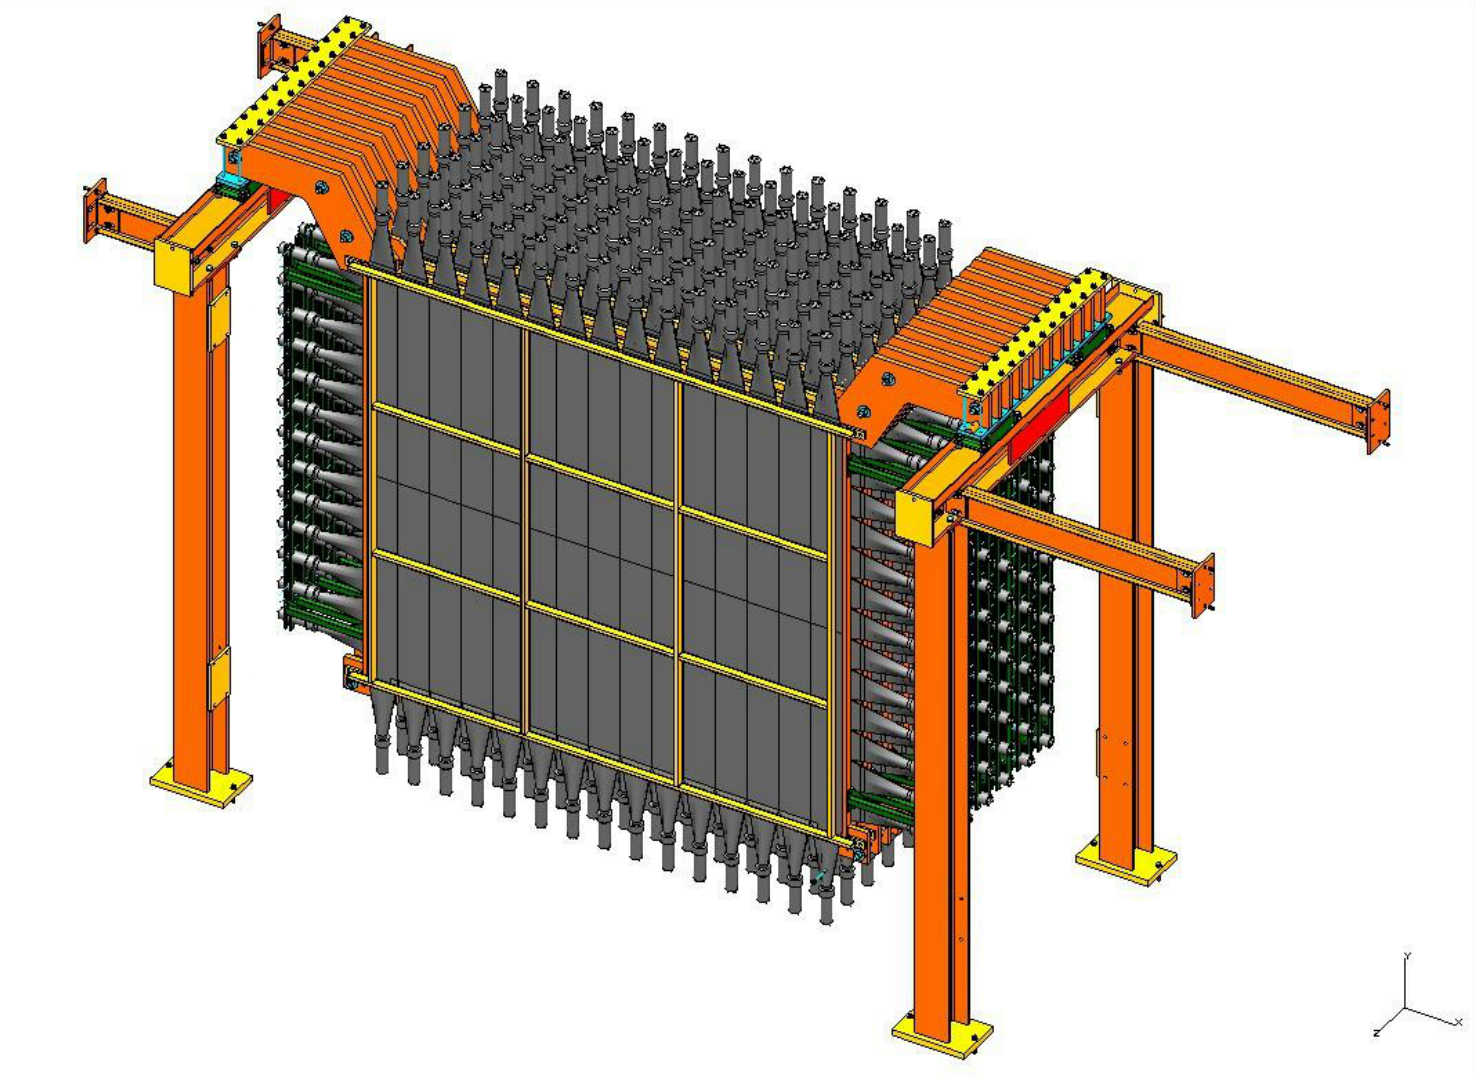
\includegraphics[scale=.15]{pics/pag23Nakajimathesis}
  \caption{Drawing of the MRD.}
  \label{fig:mrd}
\end{wrapfigure}


A fraction of the MRD will be made operational for Phase I of ANNIE in early fall.
Refurbishment activities by UC Davies will be scheduled after this phase is completed taking %
so that the detector system is fully operational in time for ANNIE first physics runs.
ANNIE will rely on a Forward Anti-Coincidence Counter (FACC) consisting of 2 layers %
of overlapping muon paddles to reject charged particles produced in dirt, upstream of the hall.
Fermilab provided a stock of 60 muon paddles taken from the CDF experiment, from which a subset %
of 26 paddles were systematically tested and selected.
These paddles have already been attached to the wall by students from UC Davis with %
the help of Fermilab technicians, using standard 80/20 aluminum extrusions and brackets, %
arranged in two staggered layers of 13 paddles each.

\begin{figure}[]
  \centering
  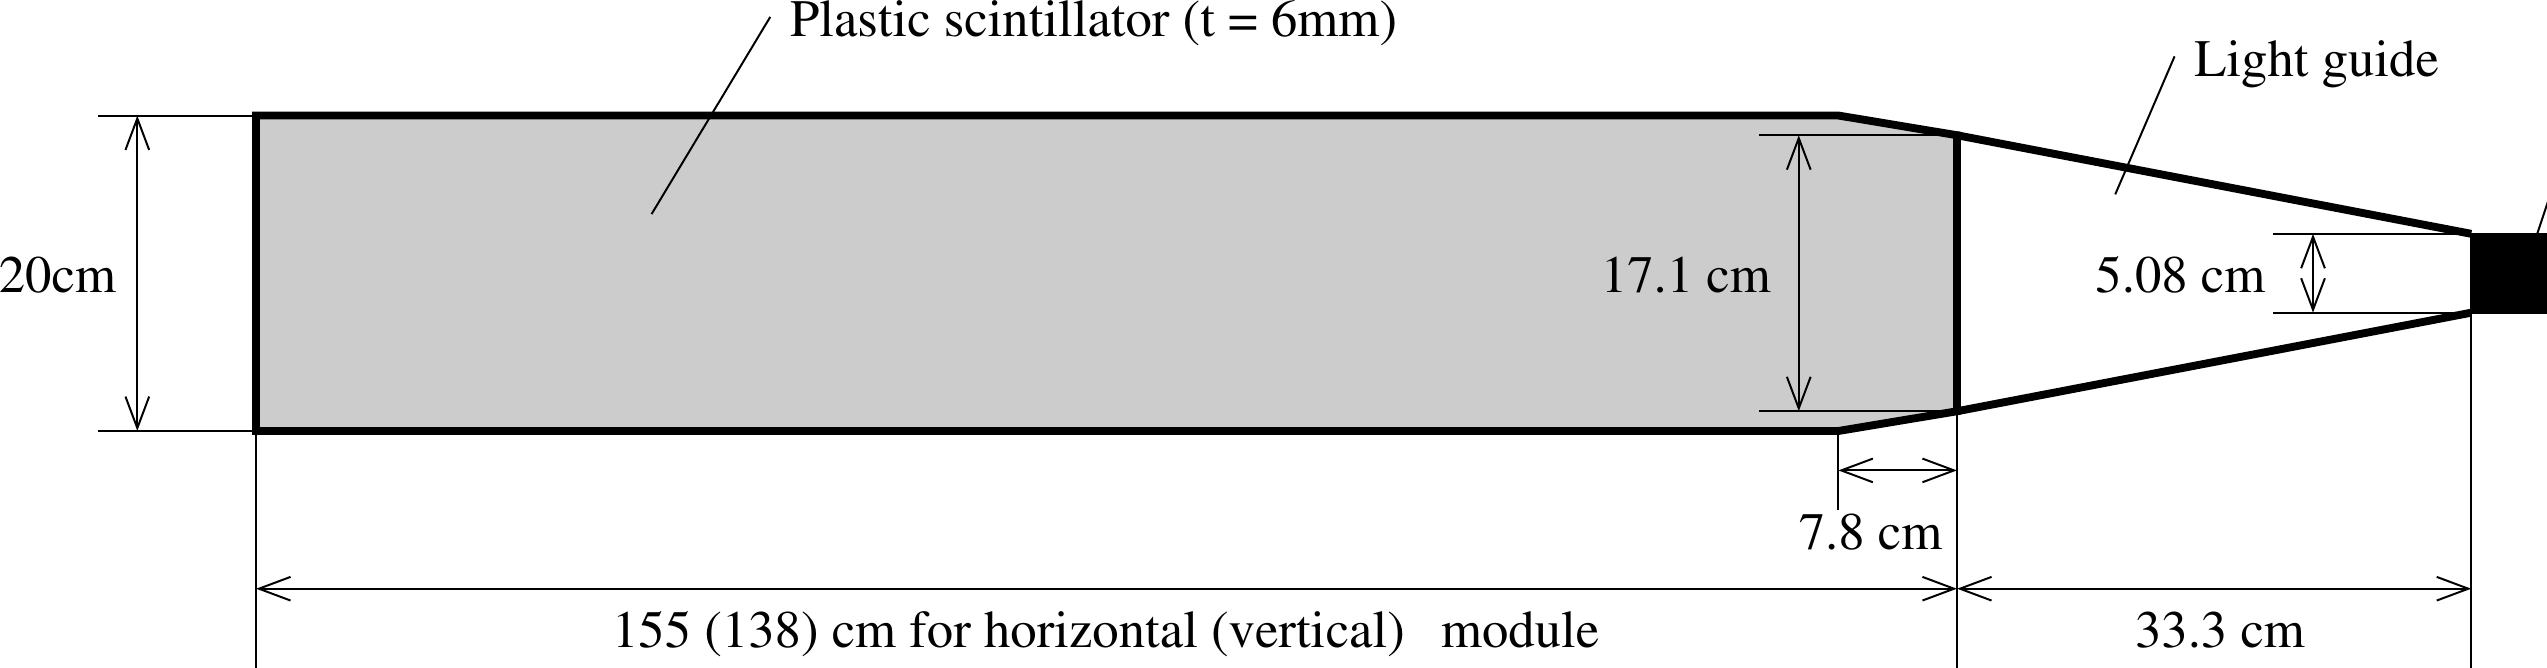
\includegraphics[scale=0.20]{pics/pag24Nakajimathesis}
  \caption{Paddle used for the MRD.}
  \label{fig:paddle}
\end{figure}

\section{Expected events}
\label{2.4}
\textcolor{red}{Odd section.}
A beam event should produce a muon in the tank, so the Veto shouldn't fire, %
some Cherenkov light could be captured by the PMTs and a clear signal is found in the MRD.

%%%%%%%%%%%%%%%%%%%%%%%%%%%%%%%		CHAP 3		%%%%%%%%%%%%%%%%%%%%%%%%%%%%%%%

\chapter[Data Acquisition]{Data Acquisition system}
\label{cha:3}

Modern high energy Physics experiment's require automated procedures to collect data from detectors %
and save them in long term storage for ensuing analysis.
These routines are gathered in automated system called Data Acquisition system (DAQ), %
which typically includes three fundamental components:
\begin{enumerate}
  \item sensors, to convert physical parameters to electrical signals;
  \item signal conditioning circuitry, to convert sensor signals into a form that %
    can be converted to digital values.
  \item conversion from analog signals to digital values and subsequent storage.
\end{enumerate}
The last step is vital in that it allows data manipulation and analysis by a computer.

As far as ANNIE is concerned, the first requirement has already been discussed in section~ref: %
the experiment has multiple simultaneous data sources, i.e. %
the forward Veto, water PMTs and the MRD, as well as a blend of front-end %
electronics technologies (VME, CAMAC and custom FADCs) for ADC/TDC and waveform digitisation.
Considering this variety of devices, the whole system has also some requirements to achieve:
\begin{itemize}
  \item stability, on long acquisition runs;
  \item control all the aspect of the experiment;
  \item calibration; 	%check this
  \item real time online monitoring;
  \item direct and remote user control.
\end{itemize}

Provided a solid electronic system, these tasks are thoroughly accomplished on the %
software's side, since the system is based upon the %
\emph{ToolDAQ Framework}\footnote{ToolDAQ %
  is open source and available on GitHub~[repo].}, developed %
by Dr Benjamin Richards~[ref] for the Hyper Kamiokande collaboration (HK).
The HK group has used this opportunity to undertake R\&D and testing of %
DAQ software and tools for future use in the HK experiment.
ANNIE experiment has allowed extensive testing of the flexibility of the software %
and all the above features to take place within a single deployment.

ToolDAQ is designed to incorporate the best features of other frameworks along with:
\begin{itemize}
  \item being very easy and fast to develop DAQ implementations in a very %
    modular way;
  \item Dynamic Service Discovery and Publishing; %
  \item scalable network infrastructure (provided by ZeroMQ) to allow its use on large scale experiments.
\end{itemize}

\begin{wrapfigure}{R}{0.5\textwidth}
  \centering
  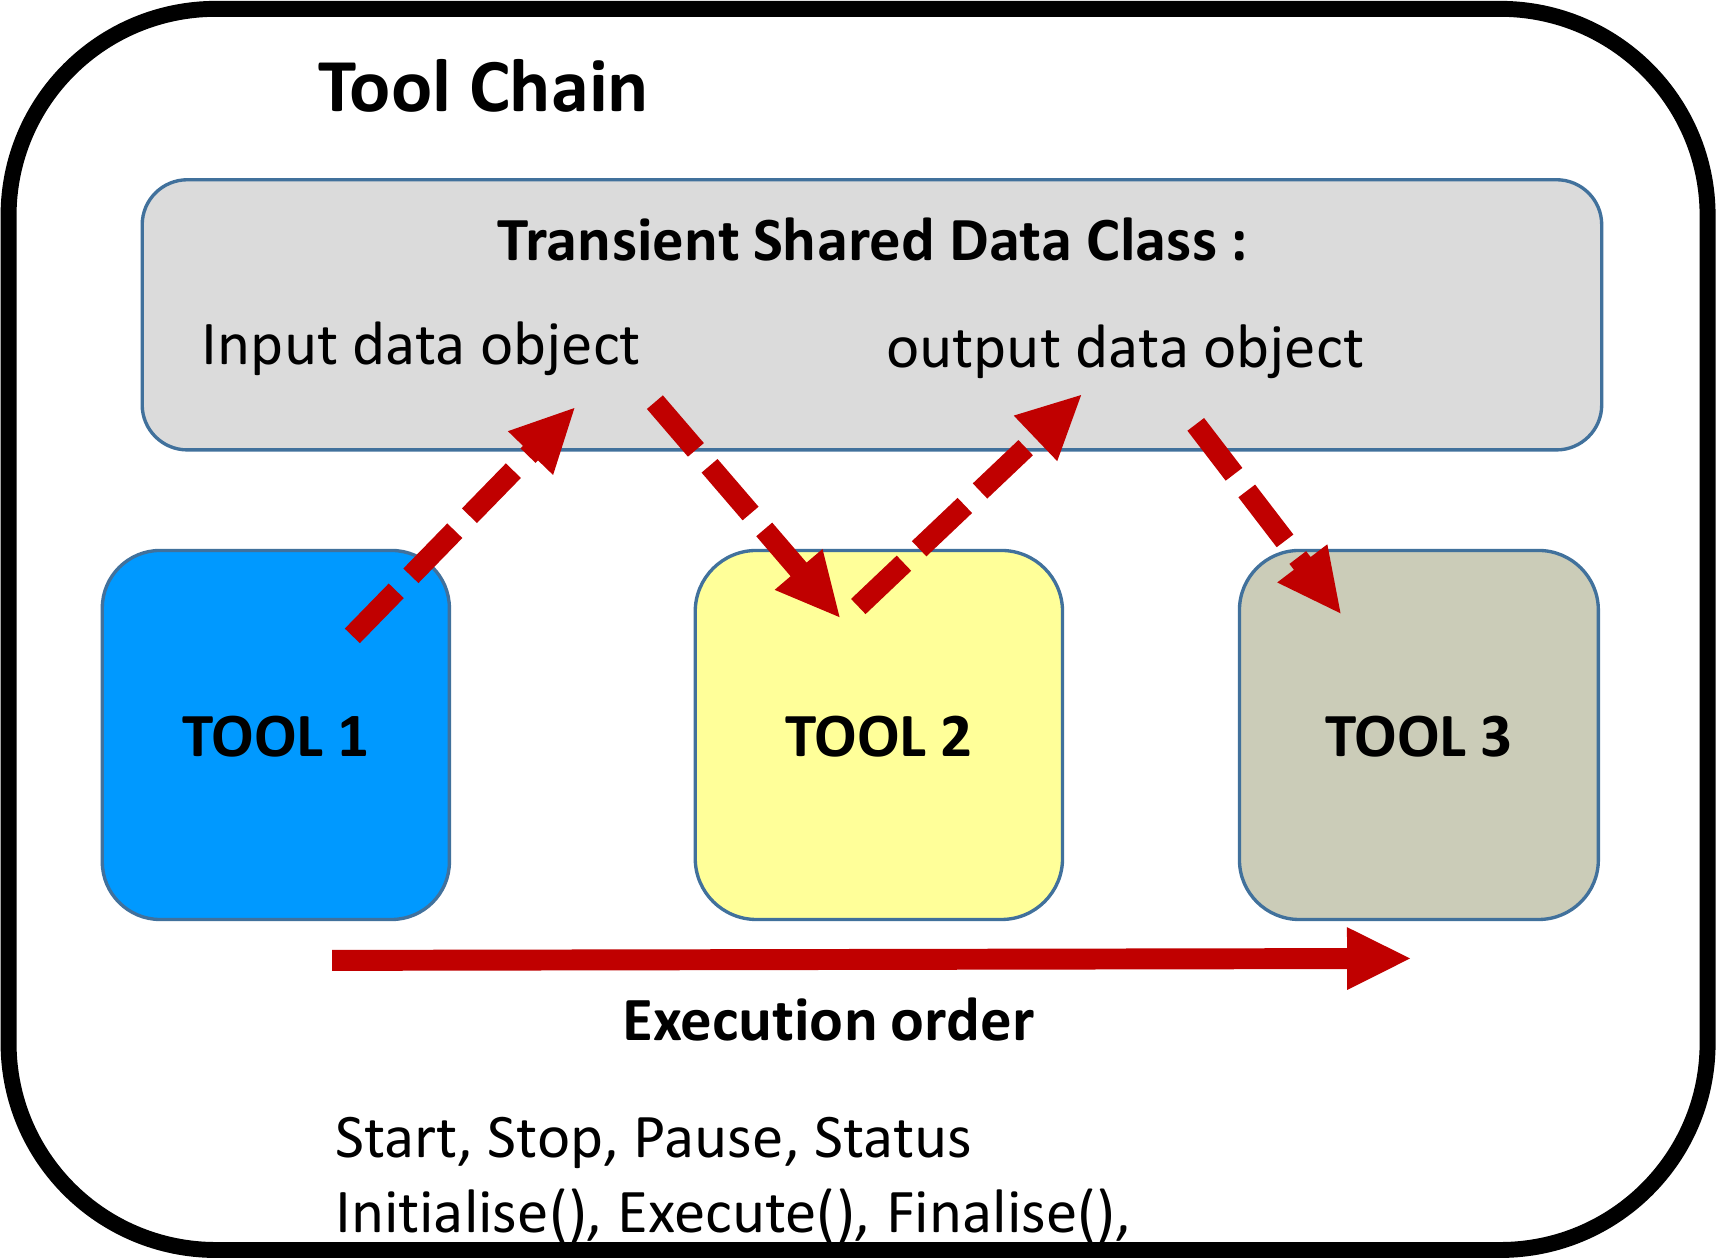
\includegraphics[scale=.13]{pics/pag4richardshkcollaboration}
  \caption{Schematic of a ToolChain.}
  \label{fig:toolchain}
\end{wrapfigure}

The main executable relies on user-defined modular classes, called \emph{Tools}, which 
present three chief functions, \emph{Initialise}, \emph{Execute}, and \emph{Finalise}.
The Tools can be daisy-chained to a \emph{ToolChain} and then handled sequentially by the process %
whenever one of those functions is called.
A ToolChain also manages the more complicated aspects of the DAQ system, %
like the remote control, the service discovery, and the status of the contained Tools.
Parameters, data and other variables are passed between Tools by an editable shared data class.
Each tool is allowed to read, update, and modify it, due to it is owned by the ToolChain.
The bare structure is sketched in Fig.~\ref{fig:toolchain}.

In the following sections, the whole DAQ structure is analysed as it currently is.
It is composed of three parallel ToolChains: the Main DAQ Chain, the VME Chain, and %
the CAMAC/MRD Chain.
The latter hasn't been implemented in the Main DAQ system yet, which is composed by the %
first two Chains only.
At the moment the MRD Chain is employed as a standalone DAQ, working in parallel %
with the Main DAQ, on a different machine with resulting difficulties.
Future integration of the two DAQ in the same machine are also discussed.

\section{Main DAQ Chain and VME Chain}

%\textcolor{red}{Improve dead time section. VME is known as CAMAC}

\subsection{Hardware}

The primary readout for ANNIE Phase I is provided by a VME-based system developed for the KOTO %
experiment\footnote{The KOTO experiment at J-PARC, Japan, aims at observing the rare kaon decay %
  $K_L\rightarrow \pi^0 \bar{\nu} \nu$ to search for new physics beyond the standard model that %
  breaks the CP symmetry. The experiment, with a new beam line and new detector components, is %
  underway and the first run was performed in May 2013.} %
by University of Chicago.
The \emph{VMEbus} is a computer architecture, where ``VME'' stands for VERSA Module Eurocard.
It is widely used in High Energy Physics due to the fact that it is of public domain and %
its data transfer speed is quite fast\footnote{For instance the latest manifestation, %
the VME320/2eSST protocol, can double the theoretical bandwidth of VME to 320MB/s.
cite[http://www.vita.com/VME320-2eSST-Protocol].}.

The crates are governed by a VME-based CPU board which runs Internet Rack Monitor software.
This latest version runs on the MVME162-22 CPU board with MC68040 CPU, 4MB dynamic ram, %
0.5MB static ram, 1MB flash memory, Ethernet interface, and support for up to four %
Industry-Pack daughter boards. 
The latter allows connection to I/O signals via ribbon cables to digital and %
analog interface boards mounted inside the IRM chassis. 
The Ethernet interface allows network connection and supports widely-used %
Internet protocols that allow data request and setting access as well as alarm reporting, %
all based upon the UDP (User Datagram Protocol) transport layer.

The system consists of two types of VME module:
\begin{itemize}
  \item 4-channel 500~MHz sampling pipeline 14 bit custom FADC cards, which primarily record %
    the traces from the PMTs in the ANNIE water volume.
  \item Master Trigger (MT) cards which distribute the 125~MHz clock, synchronises the FADC %
    cards, provides the trigger, and provides a busy signal.
\end{itemize}

The leading edge of photomultiplier signal is too fast for an 8-ns sampling.
To avoid dead time and allow the 500~MHz sampling, the output signals from the detectors %
are stored in 8000 samples pipelines inside Field Programmable Gate Arrays (FPGAs) until %
a trigger decision is made.
The three levels trigger system uses the waveform information with increased %
sophistication at each level.
Each MT card can address 8 FADC cards, but can be daisy-chained or arrange hierarchically to %
address more total cards.
Given the 16 FADC cards of the ANNIE readout, 3 MT cards are used: %
one Level-0 card distributes the clock between two Level-1 MT cards, each addressing 8 FADCs.

The Muon Range Detector and the Forward Veto nominally rely on the same FADC system as %
the PMTs in the water volume for the first runs.
The signals coming from the paddles are combined through an analog OR and sent to a %
few spare FADC channels on the KOTO boards. 

For storage limitations, a down-sampling to 125~MHz was established.
The resolution of 8~ns suffices the needs of the R\&D stage of Phase I.
An 80~$\mu$s long time window is collected, therefore with this resolution, four data sets can be %
hold in the 40000 samples buffer.
Each set corresponds to a spill from the beam.

\subsection{Software}

The data from the water PMTs and the logical sum from the Veto and MRD are acquired by the Main DAQ, %
which hinges upon two strictly complementary ToolChains: the Main Chain and the VME Chain.
The Main Chain is the primary ToolChain of the DAQ system, which communicates with the other two %
processes.

The Chain's tools are depicted in Fig.~\ref{fig:anniedaq} and they are the following:

\begin{center}
  \small
  \begin{tabular}{cc}
    \toprule
    \textbf{Main DAQ}	& \textbf{VME}		\\
    \midrule
    Input variables 		&   \\
    PostSQL 			& VME Trigger Send   \\
    Trigger			& Board Reader	\\
    Network Receive Data	& Network Send Data	\\
    Monitor			& 	\\
    Data Recorder		& 	\\
    \bottomrule
  \end{tabular}
\end{center}

The \emph{Input variables} tool loads some initialisation parameters and the specification of %
the current \emph{run}, i.e. data taking session.
Three typologies of run are available and are sent to the VME CPU: a test run, an LED run for PMTs %
calibration, a pedestal run, and a beam run.
The triggering of the digitisers is influenced by changing the kind of the run.
For instance, a beam run is triggered by the RWM, while an LED run is triggered by the LED pulser.
The \emph{PostSQL} tool updates an SQL database of the DAQ, where all the information about %
the run, such as the number of events, the start and the stop time, and others, are saved.
%Proper data logging is a fundamental step, especially for Phase I: both the experiment and the DAQ %
%are frequently revised and \textcolor{red}{knowing which run is which is pretty cool.}.
\emph{Trigger} tool blocks the Chain, awaiting and sending a trigger query from the VME.
When the VME replies, the Chain is run back again.
As explained, four 10000samples data sets are collected from the VME cards, which equates to %
four consecutive spills from the beam.
The \emph{Network receive data} tool handles the data transfer via ZeroMQ %
messaging\footnote{\emph{ZeroMQ} %
  is a high-performance asynchronous messaging library, aimed at use in distributed applications.
  The API provides \emph{sockets}, each of which can represent a many-to-many connection %
  between endpoints, operating with a message-wise granularity.
  ZeroMQ is developed by a large community of contributors and distributed under the LGPL license.
  http://zeromq.org/} %
between the main chain and the VME one.
Like most of the HEP experiments, even ANNIE requires real-time monitoring so as to check whether %
the DAQ system works flawlessly.
This is achieved by the \emph{Monitor} tool, which updates a dedicated web-page with %
random plots of data collected.

\begin{figure}[]
  \centering
  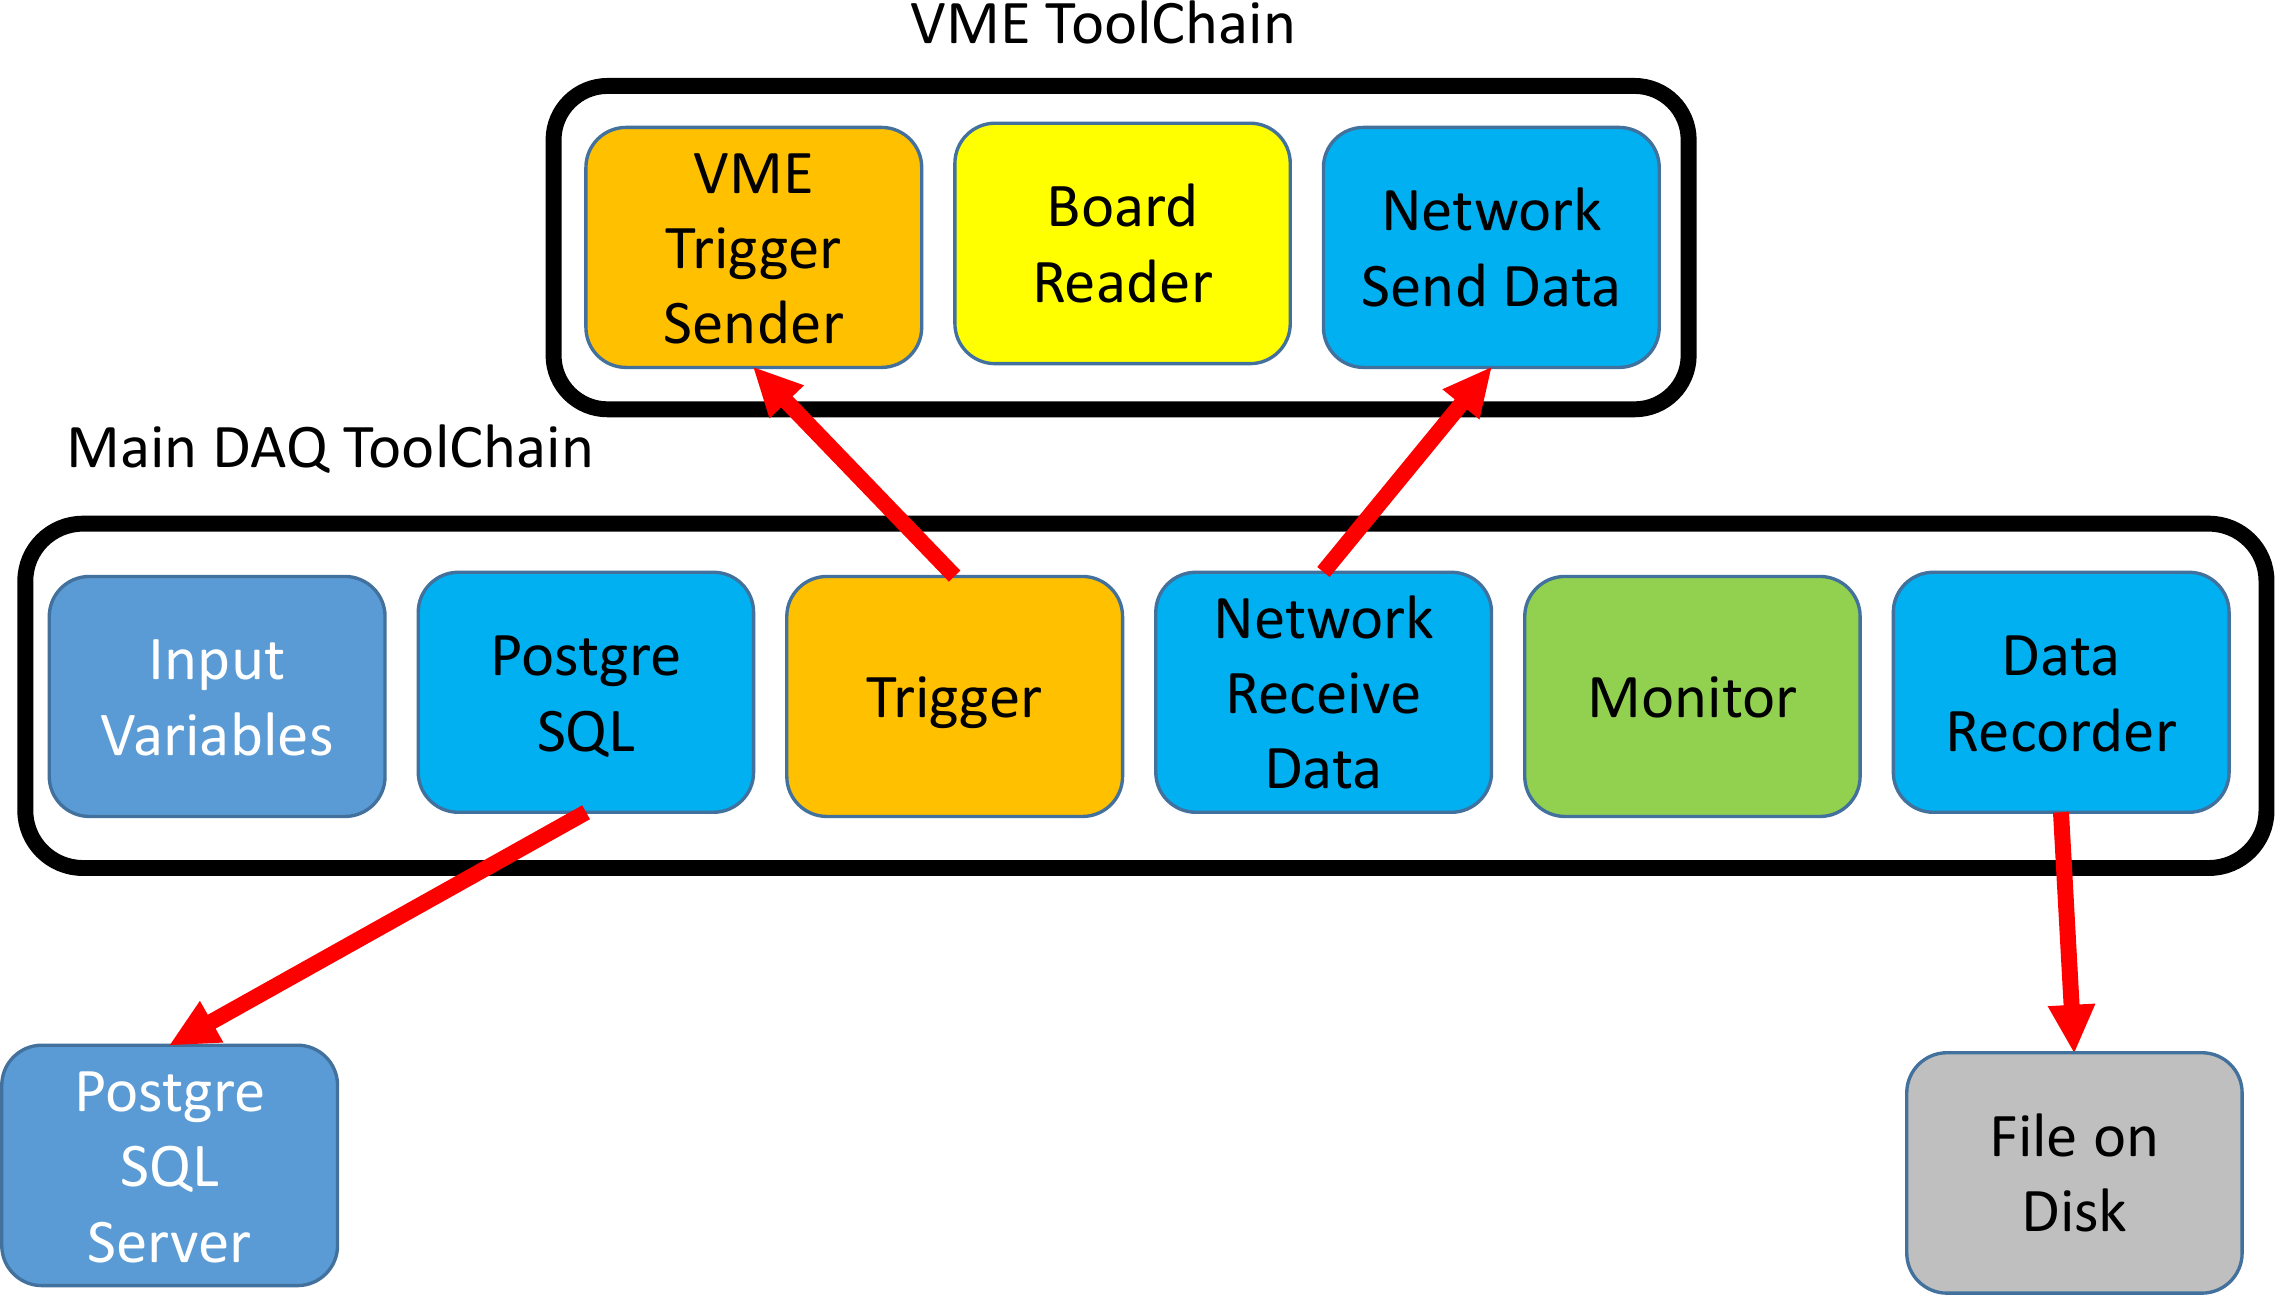
\includegraphics[scale=0.20]{pics/pag2richardshkmeeting}
  \caption{ANNIE's current main DAQ makes use of two parallel tool chains.}
  \label{fig:anniedaq}
\end{figure}

On the VME electronics side, the Chain communicates with the VME CPU retrieving all the information %
about the cards and the trigger.
The \emph{Trigger Sender} tool check the status of the VME controller.
If the ADC are triggered, a trigger message is sent to the Main Chain.
The data are dumped from the FPGA's buffer by the \emph{Board Reader} tool and %
are sent to the Main Chain via ZeroMQ messaging over TCP.

The last tool of the Main Chain, \emph{Data recorder}, saves data into the following %
ROOT tree structure:
\begin{description}
  \item[\bfseries LastSync :] time of data acquisition;
  \item[\bfseries SequenceID :] incrementale number;
  \item[\bfseries StartTime :] same as lastsync;
  \item[\bfseries CardID :] number of ADC card;
  \item[\bfseries Channels :] channel of ADC card;
  \item[\bfseries PMTID :] global identifier of PMT (labelled from 1 to 60);
  \item[\bfseries BufferSize :] size of the buffer per channel;
  \item[\bfseries FullBufferSize :] size of the buffer per card;
  \item[\bfseries Data :] an array holding the full buffer of a single card.
\end{description}

 Each entry corresponds to an acquisition of the full buffer from the cards saved in a 160000 long %
 float array, i.e. the digitised time profile of four consecutive 80~$\mu$s data set times the four channels.
 The ROOT files are then post processed: the buffer is split and an entry is created for each %
 beam event, or trigger, the baseline is calculated and removed from the time profiles, and the precise %
 time stamp is reconstructed.
 In Fig.~\ref{fig:timeprofile} an example of time profile is shown before and after the post-processing.
 Moreover, each channel is mapped to its equivalent PMT.
 This stage reduces the file sizes by a nearly a factor of four.

 Provided that the spill's frequency is $\sim$15~Hz and four spills are acquired, the buffer %
 takes around a quarter of a second to fill.
 The longest portion of the chain to execute is the disk saving and it is meant to be done %
 between pulse trains, so as to minimise the number of spills lost.
 A whole execution of the chain lasts nearly a second, slightly less than the pulse train frequency.

\begin{figure}
  \centering
  \subfloat[Before post-processing, arrays include the full buffer from each card.]%
  {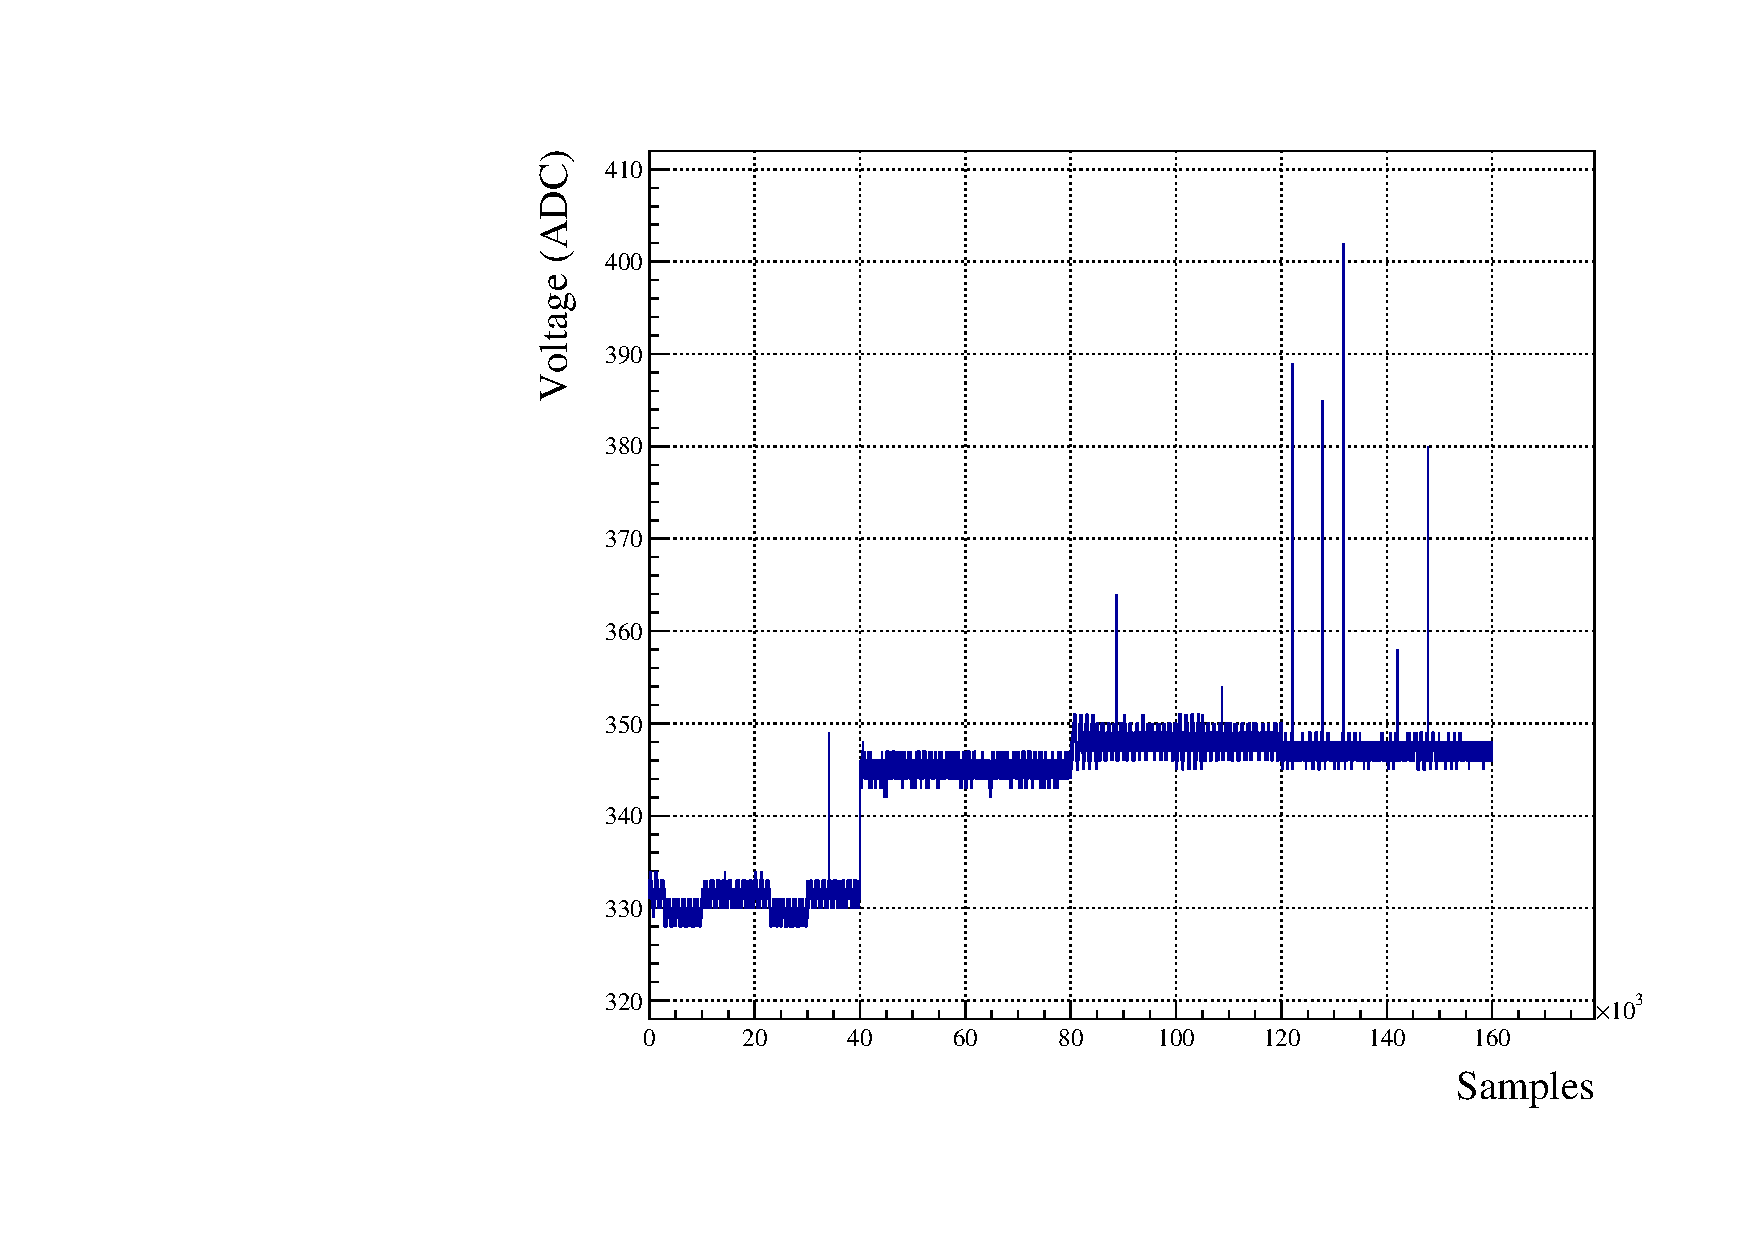
\includegraphics[scale=0.35]{pics/fullbuffer.pdf}}\,
  \subfloat[After post-processing, arrays are split per trigger and hold 80~$\mu$s worth of data.]%
  {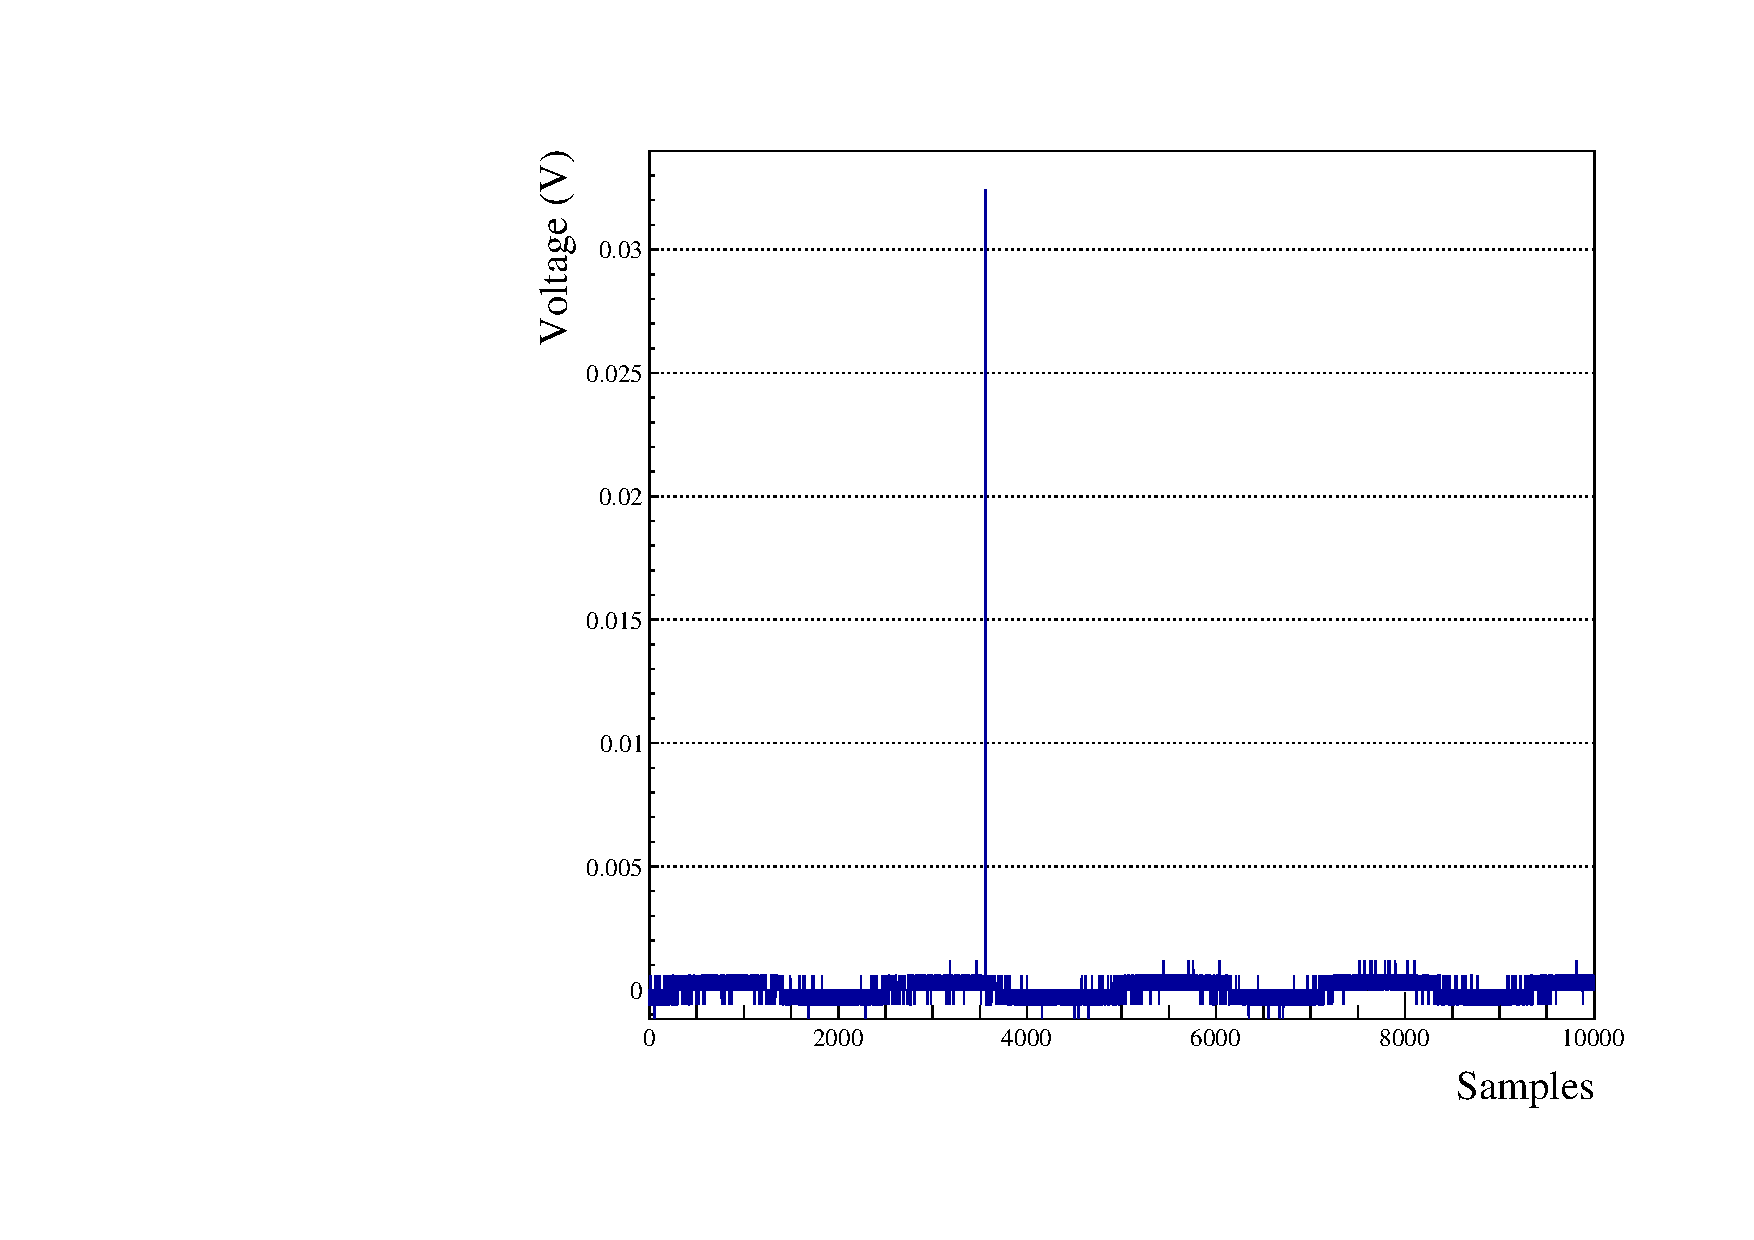
\includegraphics[scale=0.35]{pics/onetrigger.pdf}}
  \caption{Time profile before and after the post-processing.}
  \label{fig:timeprofile}
\end{figure}

\section{MRD Chain}

\label{sec:3.2}

\subsection{Hardware}

 As explained in Sec.~ref, the signal from the FACC %
 and two layers of the MRD are logically summed and read by the VME digitisers.
 The PMTs of these two detectors are supposed to be read individually by both Time-to-Digital %
 Converters (TDC) and ADCs in future stages of the experiment and for this purpose %
 a third ToolChain has been developed to collect data from both the VETO and %
 the MRD's second and third layers (see section~ref).

 CAMAC\footnote{\emph{Computer-Aided Measurement And Control} (CAMAC) is a bus and modular-crate electronic %
 standard for data acquisition and control used mainly in nuclear and particle physics experiments %
 and in industry.
 The bus allows data exchange between plug-in modules and a crate controller, %
 which then interfaces to a CPU or to a VME-CAMAC interface.} %
 electronic modules are employed for these two detectors: LeCroy 3377 modules for the time %
 digitisation, while LeCroy 4300B for analog conversion.

 The LeCroy Model 3377 is a 32-channel time-to-digital converter (TDC) and %
 optimised with a low conversion time and a high speed readout of 100~ns/word.
 With 10-bit words, the longest time window achievable is \np{4088.0}~ns, using a resolution %
 of 4.0~ns.
 A delayed signal from the RWM acts as a ``common start'' for the TDC cards and %
 each internal counter is individually stopped by hit signals.
 The channels are fed with the discriminated PMT signals of the VETO and of the second %
 and the third layer of the MRD.
 
 The LeCroy Model 4300B FERA contains 16 independent 11bit charge-to-digital converters.
 An 8-bit register and a memory containing the individual pedestal values to be subtracted from %
 each ADC are also available.
 These converters haven't been installed in the electronic chain yet.
 Nevertheless the software interface has been developed anyway.
 
 All the cards are addressed via the Weiner CCUSB controller module. 
 The CCUSB is a full-featured CAMAC Crate controller with integrated high speed USB-2 %
 interface.
 For fast data acquisition applications the CCUSB has a built-in command list sequencer, called %
 \emph{command stack} with data buffering in a 22kB size FIFO.
 A XILINX Spartan 3 family FPGA performs all CCUSB logic and functions. 

\subsection{Software}
%\textcolor{red}{Time of acquisition is 1/x. Underline that.}
 The thesis's work is mainly focused on the development of a dedicated data acquisition system %
 for the CAMAC electronics of the experiment.
 A separate MRD DAQ has been created from scratch within the ToolDAQ Framework in order %
 to acquire the MRD and the forward Veto data.
 These two detectors rely on the CAMAC electronics for front-end read out of the PMTs %
 signals and the USB controller vendor provides a C++ class to interface the controller with the %
 computer.
 
 Some C++ classes were developed with the purpose of handling more easily the modules.
 A base class takes care of opening the USB connection for the CCUSB controller and storing %
 information on the cards, such as the Slot number.
 It also allows the configuration of the command stack, i.e. the CAMAC command sequencer.
 Two derived classes implement wrapper functions to deliver CAMAC commands via the %
 NAF addressing\footnote{Module addressing is achieved knowing the slot \textbf{N}umber, %
 the sub\textbf{A}ddress, and the \textbf{F}unction code.}.

 The MRD's ToolChain employs the CAMAC classes to interface with the controller and the cards.
 As illustrated in Fig.~\ref{fig:anniedaq}, the Tools contained in the Chain are:

\begin{center}
  \small
  \begin{tabular}{c}
    \toprule
    \textbf{MRD}	\\
    \midrule
    Trigger	\\
    LeCroy 	\\
    Root output	\\
    \bottomrule
  \end{tabular}
\end{center}

 The \emph{Trigger} tool reads the FIFO of a specified card: if it is not empty, then all %
 cards presenting data are read and other tools are executed.
 Currently, a hit signal is generated in each TDCs by delaying the common start %
 signal of $\sim 1~\mu$s, such that the FIFOs are never empty in coincidence with the beam's spills.
 Three triggering behaviours are supported: external trigger, software trigger with %
 random card access, and software trigger with card test function.

 The \emph{LeCroy} tool is meant to work for both the TDCs and ADCs cards.
 If only either TDCs or ADCs are employed, then only one tool should be added in the \emph{ToolChain}.
 Otherwise, if both are used, then two \emph{LeCroy} tools are required.
 Given that the ADCs haven't been installed in the crates yet, only one tool is %
 needed for the TDCs.
 Nevertheless the charge converters have been tested, as well.
 
 The last tool fills a ROOT tree and save it to file.
 The tree has the following branches:
 \begin{description}
  \item[\bfseries Trigger :] incremental number of the trigger;
  \item[\bfseries OutNumber :] number of channels read;
  \item[\bfseries Type :] string telling whether the data refer to TDC or to ADC;
  \item[\bfseries Value :] actual value retrieved from the card.
  \item[\bfseries Slot :] slot number of the card;
  \item[\bfseries Channel :] channel of the card from which the value was retrieved;
  \item[\bfseries TimeStamp :] UNIX time stamp of the entry, since epoch, in ms.
\end{description}

 The MRD Chain runs in a different PC than the Main DAQ and the ToolChain %
 is executed at a different speed, for it is a standalone process.
 For this reason, a method has been realised to correlate the events between the two DAQs.
 Timestamps were designated for this fundamental task: both DAQs assign UNIX time to each event, since %
 the clocks are synchronised to the same NTP server, which uses GPS time sources.
 With the help of the Fermilab spill database [ref here], the events from the two DAQs can be related %
 to each other.

 This method is effective as long as the frequency of the chain execution is greater than the %
 spill frequency.
 The frequency should be above the 15~Hz spill frequency in order not to miss any beam event.
 However the CAMAC event rate has been found to be quite low in this %
 early stage, around \np{0.20}~Hz\footnote{The rate is measured from output ROOT file, dividing %
   the number of entries, i.e. events, by the time passed between the first and the last TimeStamp.}, %
 since only two layers of the MRD are used, in addition to the Veto.
 This suggest that the modules present data only the $\sim$\np{1.3}\% of the time.
 
 Concerning the MRD DAQ, the longest portion of the chain is the CAMAC addressing and data collecting.
 The software has been tested using software triggering, employing the test functions of the modules, %
 and counting the time required for \np{100000} repeated cycles with \np{1.3}\% firing probability; %
 the frequency was afterwards estimated.
 The result is shown in Fig.~\ref{fig:tdcfreq}, where frequency vs number of channel is %
 plotted for TDC modules.
 It's clear that the frequency is well above the lower theoretical limit of 15~Hz.
 Rescaling the frequency to full time firing, i.e. the number of channel to be read is maximum %
 for every DAQ cycle, the limit is easily reached with just ten modules, corresponding %
 to five layers of MRD, Veto excluded.
 
\begin{figure}
  \centering
  \import{pics/}{textdc.tex}
    \caption{DAQ frequency reading TDCs with all channels fired, but \np{1.6}\% time occupancy.}
  \label{fig:tdcfreq}
\end{figure}

 The command stack of the CCUSB controller is not employed, because the USB connection can provide %
 fast enough communication to address all the active cards.

 Concerning the TimeStamp, a time variable drift in the MRD TimeStamps has been found, %
 likely due to imprecise synchronisation with the NTP server %
 (accuracy given to be less than 30~ms) which occurs every 1024~ms. 
 A post-processor has been written to fix the TimeStamps, identifying time patterns in the %
 spill spectrum and comparing them to the database information.
 In Fig.~\ref{fig:tdcpost} a detail of the result of the synchronisation is plotted.
 The blue lines are given by the database, used as a reference.
 The TimeStamps before and after the post-processing are printed respectively in red and green.

 The post-processor also handles other aspects of the raw data, like converting the module's values %
 into physical quantities and mapping each channel to its PMT.

\begin{figure}
  \centering
  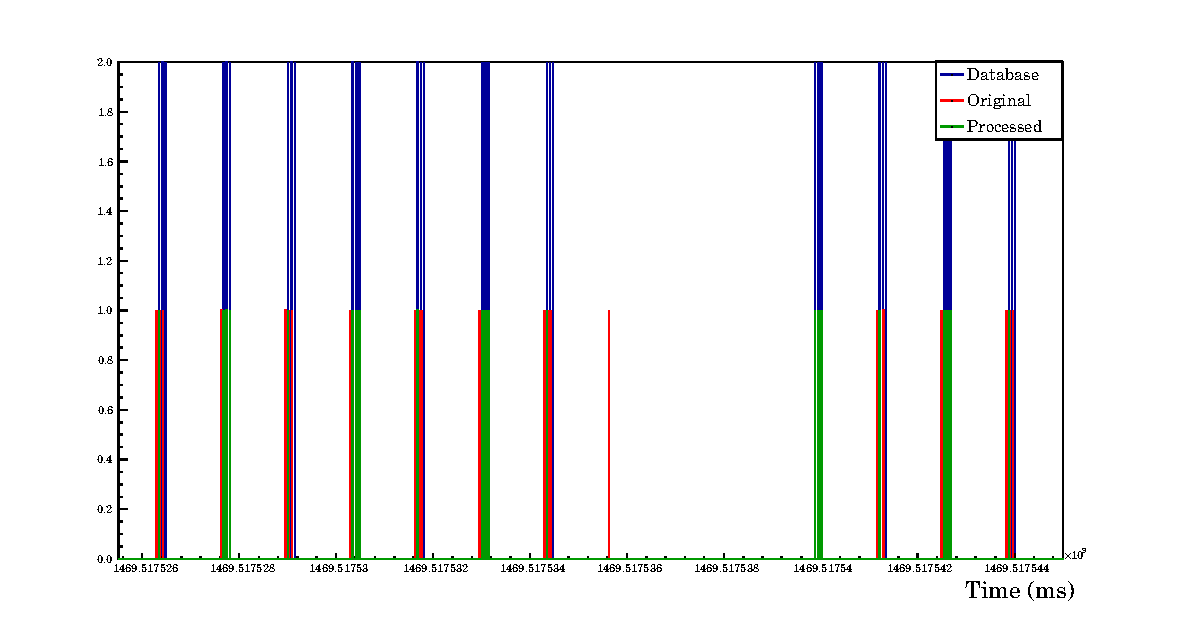
\includegraphics[scale=0.7]{pics/textime.pdf}
  \caption{Detail of the time stamp alignment with the database data.}
  \label{fig:tdcpost}
\end{figure}

\section{Future improvement}
\label{sec:3.3}

 The final version of the DAQ system needs a full integration of the Main Chain with the %
 CAMAC one.
 A possible solution is depicted in Fig.~\ref{fig:daqcomplete}.
 A new tool could be employed to embody a simplified version of the MRD ToolChain, rather than %
 run it in a parallel process.
 The MRD Chain, as proved in previous sections, is fast in execution, so it should not %
 significantly slow down the Main DAQ.
 In this way, the TimeStamp synchronisation technique is not required anymore because all the %
 acquisitions are done by the same CPU and simultaneously.
 As far as the output files are concerned, the ROOT trees could be merged into a single ROOT file %
 triggering the two recording tools with ZeroMQ communication.
 Final reconstruction of PMTs data and MRDs could be done in a post-processing stage.

\begin{figure}[]
  \centering
  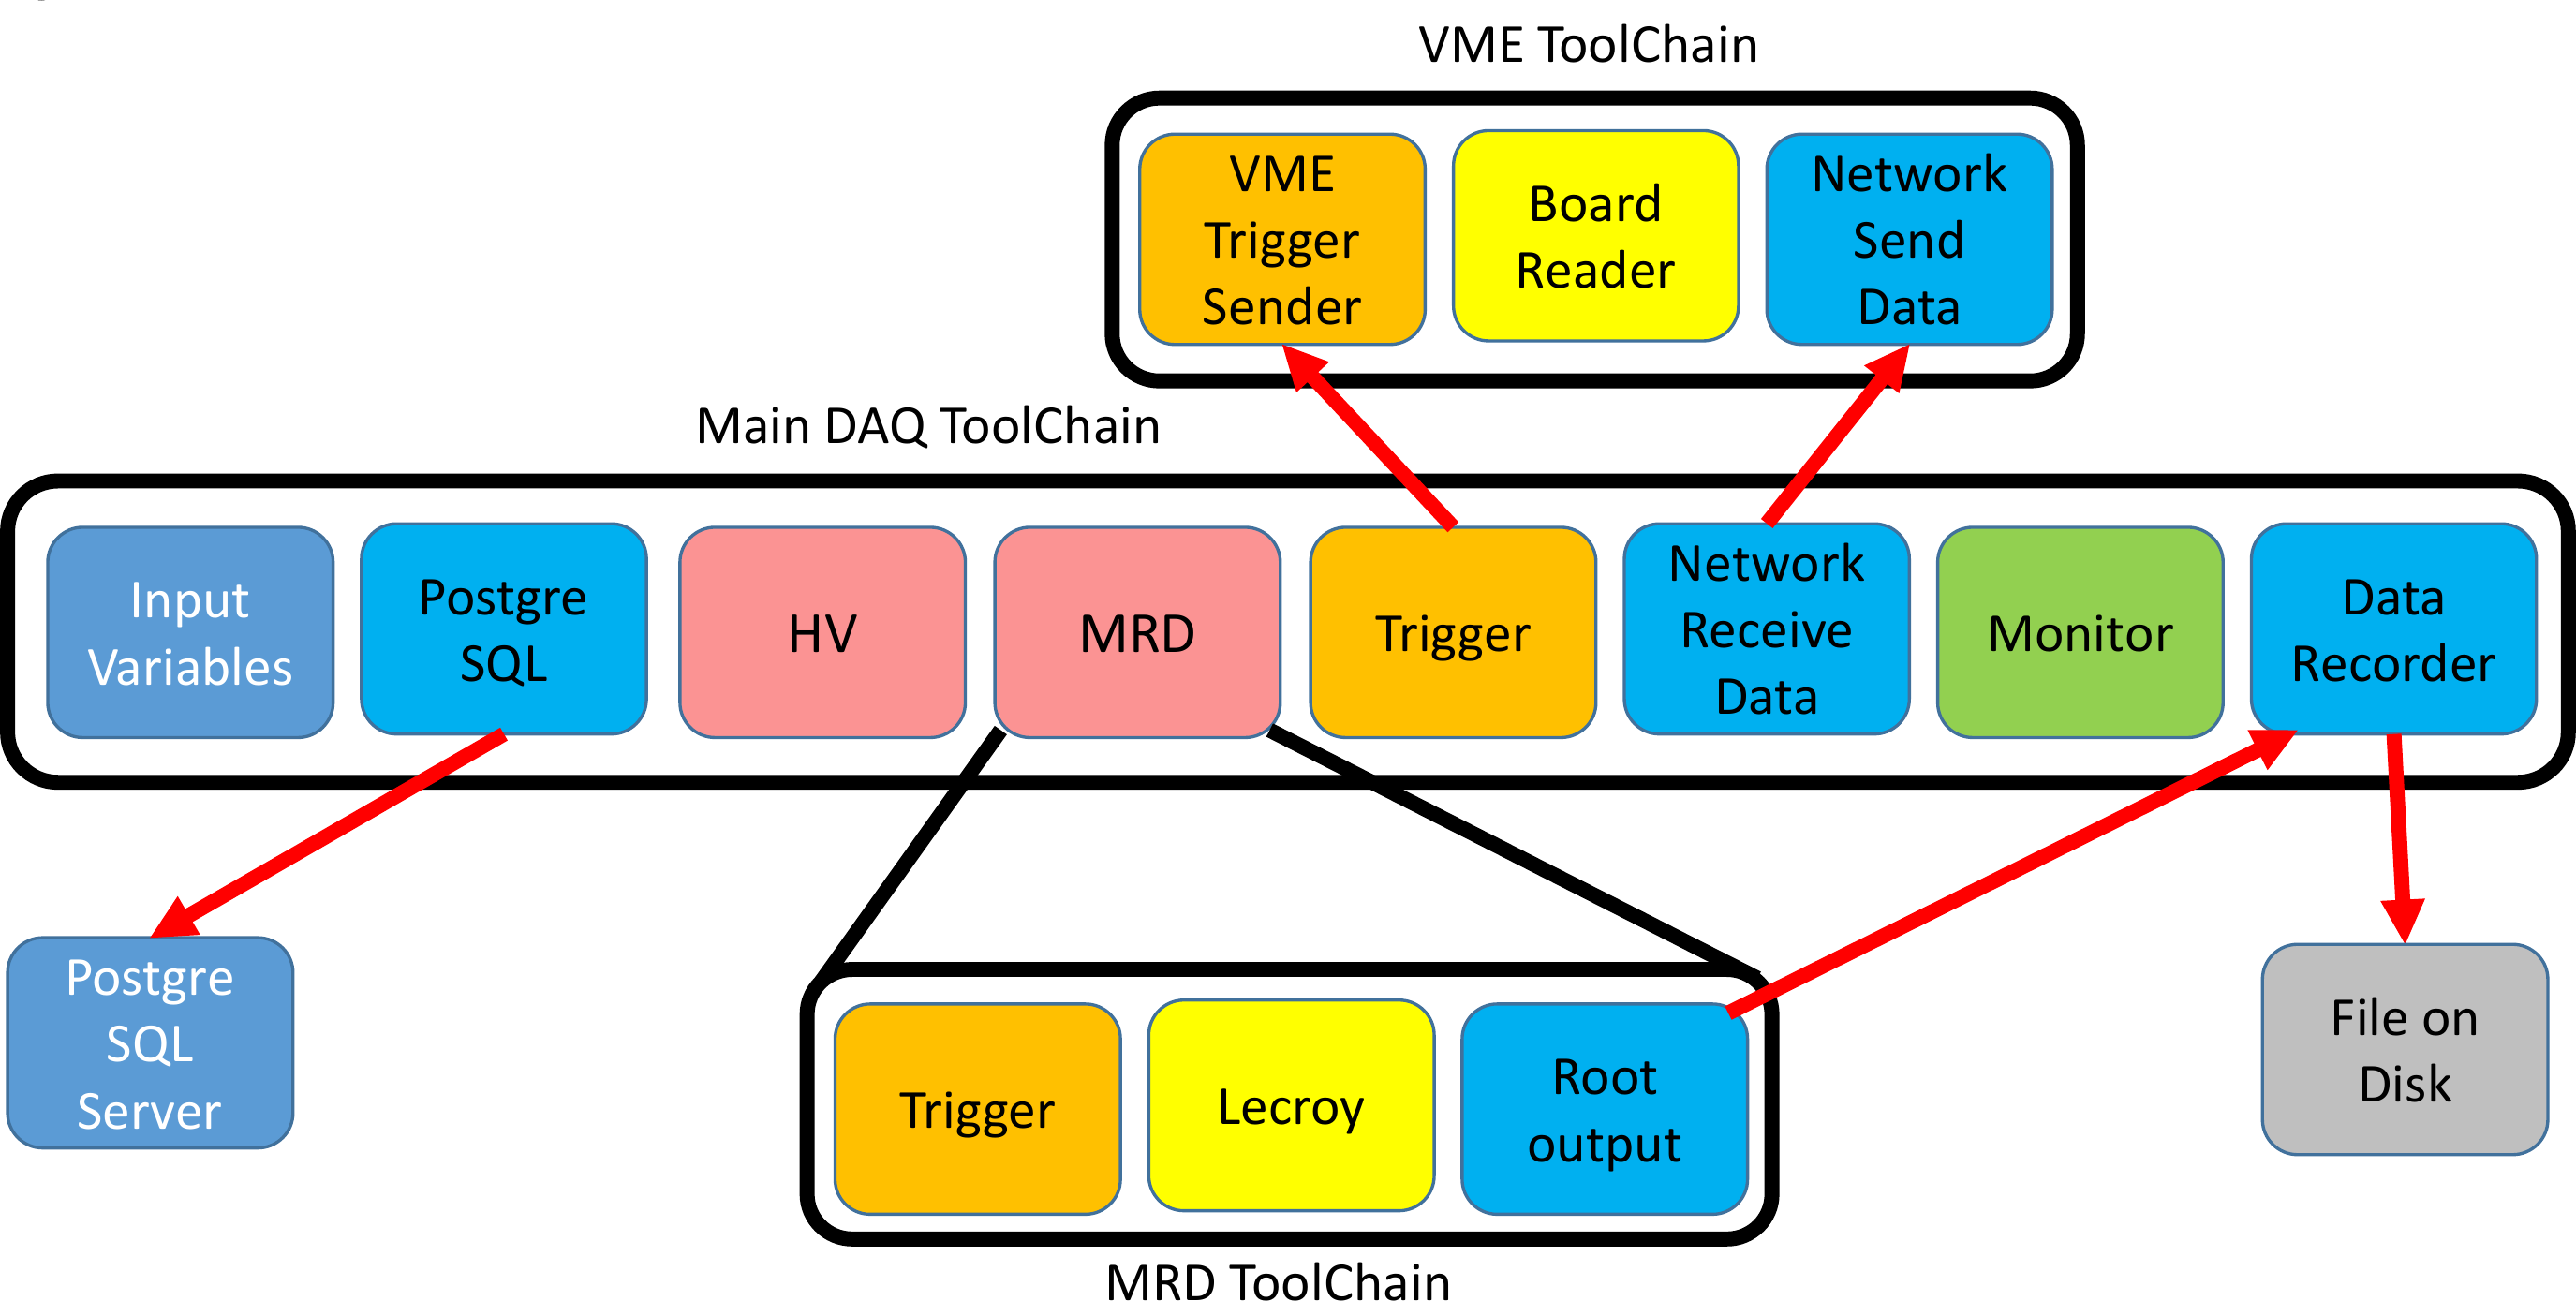
\includegraphics[scale=0.17]{pics/pag5richardshkmeeting}
  \caption{Final version of ANNIE's DAQ, with all the Chains integrated.}
  \label{fig:daqcomplete}
\end{figure}

 In view of the next phases of the experiment, an other DAQ-related issue is the memory storage.
 During early test runs, the digitiser would sample at a frequency of 500~MHz, but it has been %
 promptly downgraded to 125~MHz because of lack of long term memory storage.
 As a matter of fact, noise is mostly shown in the 80~$\mu$s time window and %
 the meaningful signal is limited short, compared to the time window.
 Considering that an high time resolution is pointless in the R\&D stage of the experiment, the %
 downgrade was established.
 Soon, \emph{zero-suppression} method would be employed, which will definitely overcome storage needs.
 The preliminary data analysis undertaken can back this decision up, as explained in section~[ref].

%%%%%%%%%%%%%%%%%%%%%%%%%%%%%%%		CHAP 4		%%%%%%%%%%%%%%%%%%%%%%%%%%%%%%%

\chapter{Data Analysis procedures}
\label{cha:4}

 Interpreting the electronic signals produced by the detector is a mandatory step for event reconstruction %
 process.
 Energies, momenta, and directions of the involved particles must be established in order to determine %
 the detected physical interaction, whose study is the ultimate goal of the experiment.
 ANNIE's early stage data have been studied and analysis algorithms were developed and tested from scratch: %
 they are implemented in a purpose-built software, which studies the signals acquired from the water PMTs.
 The code's procedures relies on individual pulse analysis and it is largely focuses on the rejection of %
 background with respect to event signals.
 Some of these methods, illustrated, in this chapter could be employed into a more complete analysis %
 framework, valid even for the future phases of the experiment.

\section{Data selection}

 The Main DAQ is programmed to create a new \emph{Run} every time the Chain is stopped and restarted.
 Due to being an R\&D phase, the DAQ has been improved in various occasion during data taking, %
 hence the size and the number of post-processed files, that constitute the \emph{Runs}, are not constant.
 Nevertheless high statistics were achieved most of the time.
 The post-processed ROOT files (see section~ref) from the DAQ are used in the data analysis.
 The buffer retrieved from the VME boards is properly split for each trigger (hardware or software) signal, %
 in that each set of data consists of 80~$\mu$s worth of digitised signal.
 A single file holds 383 full buffers and this translates to 1532 triggers, or physically speaking to \np{122.560}~ms.

 Two distinctive couples of consecutive runs were selected as model data set, with the intention to %
 outline the best data analysis procedures.
 These are:
\begin{itemize}
  \item two runs with the beam off and a random trigger: these data are mostly \emph{cosmics};
  \item two runs with the \emph{beam} on, but with one PMT mounted on top of the NCV, in order to %
    observe the neutron capture.
\end{itemize}

 All the couples have been merged in single files after being scanned by the data analysis algorithm and %
 so treated as ones.
 Their quantitative features are shown in Tab.~\ref{tab:runs}.
 For the analysis's sake, the \emph{beam} and the \emph{cosmics} data set are the same, but for a different %
 photodetector.

\begin{table}
  \caption{Runs selected for data analysis. They are composed of different numbers of file, resulting in %
    diverse number of triggers. Total time is the number of triggers times 80~$\mu$s.
    The listed memory sizes refer to the post-processed files.}
  \label{tab:runs}
  \small
  \centering
  \begin{tabular}{crcrr}
    \toprule
    \textbf{Run type} & \textbf{N of files} & \textbf{N of Triggers} & \textbf{Total time} & \textbf{Data size} \\
    		 &      	&		& (ms)			& 	(MB)	            	\\
    \midrule	                                                                     
      Cosmics	 & 142	& \np{217544}	& \np{17403.520}	& \np{106130.447}	\\
      Beam	 & 164	& \np{251248}	& \np{20099.840}	& \np{122542.009}	\\
    \bottomrule
  \end{tabular}
\end{table}

\section{Individual pulse analysis}
%\textcolor{red}{Peak to valley suggests that a reflection occurs. Explain here or next?}

 The data analysis software scans all the post-processed time profile which the \emph{Run} consists of, %
 as the one shown in Fig.~\ref{fig:profile}, sorted by trigger and PMT number.
 Any peak above a certain voltage threshold, $V_T$, is selected and an enclosing time window %
 of a predefined length, $L$, is trimmed around it.
 A length of $L = 100$~samples was chosen, resulting in a \np{0.8}~$\mu$s long window.
 The position of the peak inside this window was set to 20\% of its length, i.e. the peak is always %
 set at \np{0.16}~$\mu$s from the beginning of the time window.
 These subsets of data are called \emph{pulses} and are collected in another ROOT file.
 The choice of window length and the peak position is the result of a compromise between speed of the code, %
 memory usage and loss of physical information.
 In fact, many pulses shows consecutive multiple peaks, as the one in Fig.~\ref{fig:pulse}, mainly given by %
 light reflections in the water tank.

 \begin{figure}
   \centering
   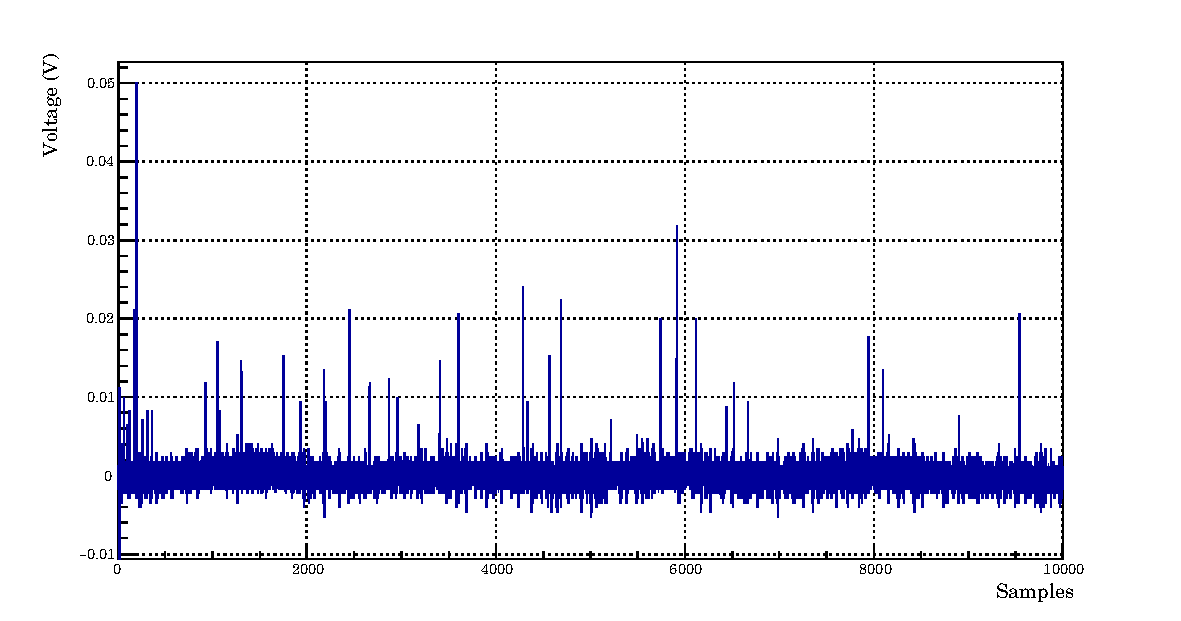
\includegraphics[scale=0.5]{pics/timeprofile.pdf}
   \caption{Time profile of a single trigger: the signals of the sixty PMTs are here overlaid.}
   \label{fig:profile}
 \end{figure}

 \begin{figure}
   \centering
   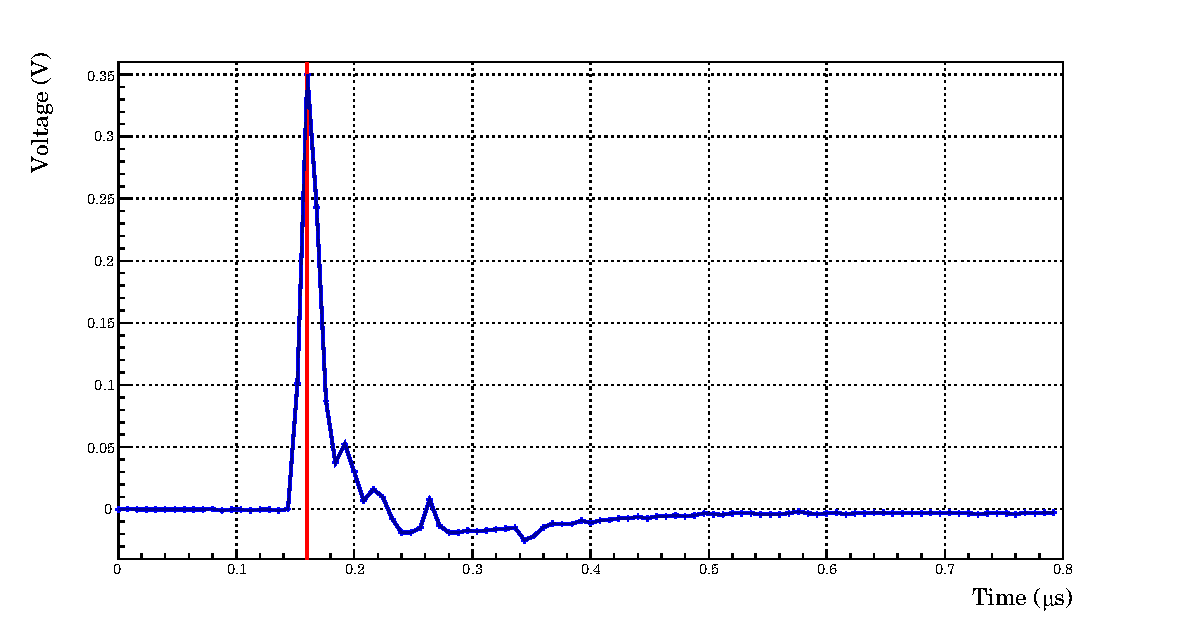
\includegraphics[scale=0.5]{pics/pulse.pdf}
   \caption{Time profile of a single pulse. The red line marks the 20\,\% of the window's length, at $\np{0.16}~\mu$s. %
     The first peak and the second peak are about forty nanoseconds apart, which is the time needed for the light to %
   travel back and forth inside the tank (see section~ref).}
   \label{fig:pulse}
 \end{figure}

 Each pulse is individually analysed and processed by a routine of algorithms.
 As a result, a set of values is gathered from every pulse, in addition to Veto and MRD coincidences.
 These quantities, outlined in Fig.~\ref{fig:pulseana}, are useful for following analysis and they are labelled:

\begin{description}
  \item[\bfseries Baseline]: it is the average of first 10 points of the pulse; %
    this value is then subtracted from the whole array.
  \item[\bfseries Height]: it is the height of the peak (maximum) with respect to the zero.
  \item[\bfseries Peak to valley]: it is the time distance from the peak to the valley (minimum).
  \item[\bfseries Start]: it is the position of the 25\% of the rising edge of the pulse, estimated with %
    precision using cubic interpolation
  \item[\bfseries Width]: it is the time that spans from Start to the 5\% of the falling edge %
    of the pulse (End), calculated using the same algorithm employed for Time.
  \item[\bfseries Charge]: it is the sum of the 5 points around peak, weighted with the bin width.
  \item[\bfseries Energy]: it is the signal integral form the Start to the End.
  \item[\bfseries Area]: it is the area of the modulus of the pulse.
  \item[\bfseries Time of flight]: is the time difference between the Start and RWM signal.
  \item[\bfseries Previous]: is the time difference between the Start and the Start of the previous pulse, %
    if from the same PMT.
\end{description}

\begin{figure}
  \centering
  \def\svgwidth{0.47\textwidth}
  \subfloat[From left to right: in green the \emph{BaseLine}, in orange the \emph{Peak Height}, %
  in purple the \emph{Width}, and in light blue the \emph{Peak to Valley} time distance.]%
  {\import{pics/}{timepoints.pdf_tex}} \qquad
  \def\svgwidth{0.47\textwidth}
  \subfloat[From left to right: in pink the \emph{Charge}, in blue the \emph{Energy}, and in gold the \emph{Area}. %
  These three integrals cross over each other in the purple region.]%
  {\import{pics/}{areapoints.pdf_tex}}
  \caption{Illustration of the pulse analysis values. The \emph{25\,\%} and \emph{5\,\% peak height} marks, %
  which define the \emph{Start} and \emph{End} of the signal, are common to both diagrams. The dashed lines represent %
  the cubic interpolations.}
  \label{fig:pulseana}
\end{figure}

 Being a water Cherenkov detector, the event reconstruction in ANNIE relies on time and energy of the signals %
 and for this fact these two quantities must be measured precisely.
 The time position of the pulses, or \emph{Start}, is thus determined with high precision thanks to data %
 interpolation\footnote{The algorithm looks for four points around the threshold (25\,\% for the \emph{Start} %
   or 5\,\% for the \emph{End}), which are used to define a cubic function. Using Newton's method, the correct %
   time position is found.}, within the time resolution of the ADCs.
 In Fig.~a of~\ref{fig:spectrum} the spectrum of the \emph{Starts} of a beam run is plotted: the frequency boost %
 with respect to the background suggests that the beam occurs ten microseconds after the beginning of the data %
 acquisition.
 The distinctive trait of the neutron capture by gadolinium is a delayed signal, detected 20-30~$\mu$s.
 Therefore studying the relative time distance between pulses is fundamental, particularly in the ANNIE experiment.
 The \emph{Previous} entry has the potential to accomodate this neccessity and reveal other interesting features.
 For instance, in Fig.~b of~\ref{fig:spectrum} \emph{Start} is plotted against \emph{Previous}.

 \begin{figure}
   \centering
   \subfloat[The beam is clearly visible at the beginning of the 80~$\mu$s buffer; the second half is basically free of %
   beam related events. ]{\includegraphics[width=0.47\textwidth]{pics/timefreq.pdf}}\,
   \subfloat[\emph{Start} is plotted against \emph{Previous}; both axes are in $\mu$s.
   The beam pulses are split into two groups: the pulses in the red ellipse are independent of their previous pulse, %
   while a correlation is visible in the set of the blue ellipse.]%
   {\includegraphics[width=0.47\textwidth]{pics/startvsnext.png}}
  \caption{Time distribution of the pulses of a beam run.}
   \label{fig:spectrum}
 \end{figure}

 On the other hand, estabilishing the signals' energy is more complicated, since the PMTs have not been calibrated yet.
 However, the photodetectors are set with the same gain, therefore an evaluation of the pulse integral is a good %
 indicator of the total charge deposited on each PMT.
 Three different methods to estimate the area enclosed in a pulse integral have been implemented.
 The names \emph{Charge}, \emph{Energy}, and \emph{Area} were only chosen in order to distinguish them from each other.
 As suggested from Fig.~\ref{fig:pulse}, there is a partial superimposition of the three: they show indeed %
 interesting correlation patterns, reported in Fig.~\ref{fig:integral}.

\begin{figure}
  \centering
  \subfloat[The \emph{Charge} is plotted against the \emph{Energy}]%
  {\includegraphics[width=0.47\textwidth]{pics/chargevsenergy.png}}\,
  \subfloat[The \emph{Area} is plotted against the \emph{Energy}]%
  {\includegraphics[width=0.47\textwidth]{pics/areavsenergy.png}}\\
  \subfloat[The \emph{Area} is plotted against the \emph{Charge}]%
  {\includegraphics[width=0.47\textwidth]{pics/areavscharge.png}}
  \subfloat[The spectrum of \emph{Width}.]%
  {\includegraphics[width=0.47\textwidth]{pics/width.pdf}}
  \caption{Correlation plots among the three integral quantities. The red lines isolate areas with different %
  correlation, likely due to different widths of the pulses.}
  \label{fig:integral}
\end{figure}

 For every Trigger, the time distribution of the peaks is studied, as well as the time coincidences %
 between the PMTs signals: a time allowance of $\np{0,8}~\mu$s is considered to count of pulses happening %
 simultaneously; this easily translates to the number of PMTs fired at the same time.
 When the latter exceeds a defined threshold, $N_{PMT}$, then an \emph{Event} is appointed and its precise time %
 position is afterwards estimated by a weighted average of the adjacent coincidences.
% The time tolerancy is high enough to include most of the in a way that all the light from the interaction is counted
 The multiplicity of an Event is a good indicator of the nature of the detected interaction.
 As discussed in section~ref, a cosmic muon, likely coming from above, would project the Cherenkov radiation on the %
 bottom of the tank, thus lighting the majority of the water PMTs.
 On the other hand, a muon arisen from the interaction of a beam neutrino with a nucleon would emit gammas %
 along the beam direction: only a portion of the light cone could be captured, hence the PMTs would be partially %
 triggered.
 Even natural radioactivity, from radionuclide in the glass of the phototubes, can be detected, although %
 these events have lower multiplicity and are readily filtered by a proper threshold of $N_{PMT}$.
 An high-multiplicity event is exemplified in Fig.~\ref{fig:event}.

  \begin{figure}
   \centering
   \subfloat[The red line marks the weighted average of the coincidences, which is $\np{34.51}~\mu$s in this example.]%
   {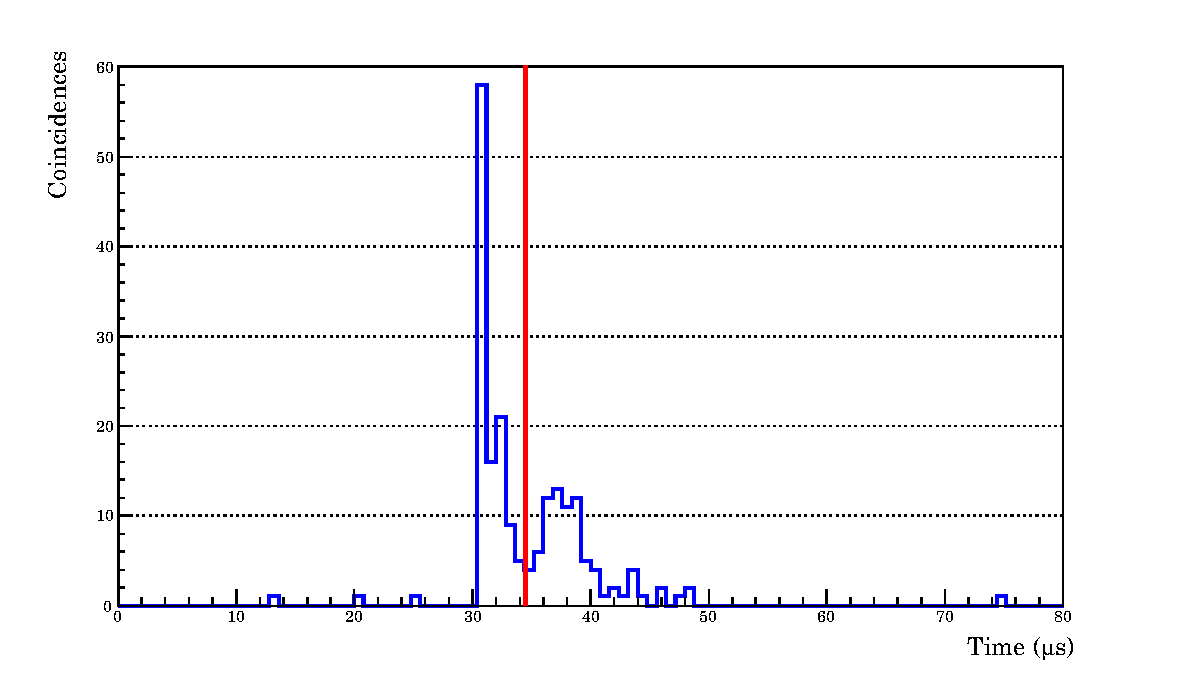
\includegraphics[width=0.47\textwidth]{pics/coincidences.pdf}}\,
   \subfloat[The coloured lines mark the five time window for noise rejection, $\Delta_T$ in $\mu$s, %
   listed in Tab.~\ref{tab:thr_var}.]{\includegraphics[width=0.47\textwidth]{pics/rejection.pdf}}
   \caption{Both plots show the same histogram, filled with the \emph{Start} time of each pulse belonging to %
   the same trigger. An high multiplicity event is found near $\np{31}~{\mu}$s.
   In this particular case, the time distribution of the signals is quite long: %
   the light in the tank lasts for about twenty microseconds.}
   \label{fig:event}
 \end{figure}

 Not every pulse in a trigger belongs to an event.
 For instance, in Fig.~\ref{fig:event} there are at least four pulses outside from the main pulse cluster.
 These might be likely generated by noise sources and therefore they are useless in view of the event %
 reconstruction.
 In order to discriminate the pulses, an arbitrary time interval, whose radius is $\Delta_T$, is defined around %
 the Event time position.
 Every pulse that falls within this window is designated as a \emph{signal}; otherwise it is \emph{noise}.

\section{Signal and noise discrimination}

 Discriminating signal from background is a step of utmost importance for data analysis.
 Being a first stage study, the algorithm only relies on $V_T$, $N_{PMT}$, and $\Delta_T$, %
 in order to distinguish event pulses from noise ones.
 It is necessary, even for future analysis framework, to determine the best combination of the three parameters.
 To achieve that, these have been varied and the data have been analysed multiple times.
 Twelve combination were chosen and they are listed in Tab.~\ref{tab:thr_var}.
 The variation of the voltage threshold affects the total number of pulses, because any peak below $V_T$ is %
 neglected.
 The five values employed are all well above the electronic noise, which is of the order of the millivolt.

 The ratio between \emph{signals} and \emph{noises} is rather governed by the other two parameters, %
 the number of PMTs fired and the rejection time window.
 Respectively four and five values were picked for these parameters.
 The increase of $N_{PMT}$ restricts the number of \emph{events}, as suggested by Fig.~\ref{fig:npmt} where the %
 multeplicity of the events is plotted.
 This values is indeed closely related to the number of PMTs hit in an interaction.
 The rise in the frequency, near the end of the x-axis, is likely due to high multeplicity cosmic muon events.
 The time allowance of the \emph{event} definition was also studied, varying the $\Delta_T$ parameter.
 Understanding the relevance of belated photons, possibily given by reflection inside the tank, is decisive for %
 developing a correct analysis framework.
 The selected intervals are illustrated in Fig.~b of~\ref{fig:event}.

 \begin{figure}
   \centering
   \includegraphics[width=0.5\textwidth]{pics/pmt.pdf}
   \caption{Frequency of the number of PMTs hit in an event.}
   \label{fig:npmt}
 \end{figure}

% \begin{wraptable}{r}{0.5\textwidth}
 \begin{table}
  \caption{The combination of the employed thresholds.
    The first one, in bold letters, is common to each subset.}
  \label{tab:thr_var}
  \centering
  \small
  \begin{tabular}{lccc}
    \toprule
    \textbf{Label}	& $V_T$		& $N_{PMT}$		& $\Delta_T$	\\
    	&	(V)	 		& 			& ($\mathrm{\mu}$s)			\\
    \midrule
    $C$	&	\textbf{\np{0.02}}	& \textbf{10}		& \textbf{\np{4.0}}		\\
    \midrule
    $V_{00}$	&	    \np{0.005}		& 10			& \np{4.0}			\\
    $V_{01}$	&	\np{0.01}		& 10			& \np{4.0}			\\
    $V_{05}$	&	\np{0.05}		& 10			& \np{4.0}			\\
    $V_{10}$	&	\np{0.10}		& 10			& \np{4.0}			\\
    \midrule
    $N_{15}$	&	\np{0.02}		& 15			& \np{4.0}			\\
    $N_{30}$	&	\np{0.02}		& 30			& \np{4.0}			\\
    $N_{50}$	&	\np{0.02}		& 50			& \np{4.0}			\\
    \midrule
    $\Delta_{50}$	& \np{0.02}		& 10			& \np{5.0}			\\
    $\Delta_{30}$	& \np{0.02}		& 10			& \np{3.0}			\\
    $\Delta_{20}$	& \np{0.02}		& 10			& \np{2.0}			\\
    $\Delta_{10}$	& \np{0.02}		& 10			& \np{1.0}			\\
    \bottomrule
  \end{tabular}
 \end{table}
 %\end{wraptable}

 The processed data sets present therefore different number of pulses and different proportion between signals %
 and noises.
 Every collection of processed data is then studied a posteriori and tested with diversified methods. 

%%%%%%%%%%%%%%%%%%%%%%%%%%%%%%%		CHAP 6		%%%%%%%%%%%%%%%%%%%%%%%%%%%%%%%

\chapter{Data analysis results}
\label{cha:5}

 In this chapter, the data analysis results are presented.
 Using the techinques described in the previous section, the selected data sets are %
 studied (see section~ref) in order to test the validity of the selection method proposed.
 The rate of comsic is also evaluated, as well as the muon lifetime and the neutron yield %
 \textcolor{blue}{(not sure about this lol)}.

\section{Cosmic background data}

 High energy particles, mainly originated outside the Solar System and thus called %
 \emph{Cosmic Rays}, impact on the Earth's atmposhere and producing mesons, which in turn generate %
 secondary particle shower by decaying.
 The primary particles are about 99\,\% made of ionised nuclei (79\,\% protons, 19\,\% alphas, 2\,\% %
 heavier nuclei), while the remaining 1\,\% is mostly composed by electrons.
 The intensity of the nucleons in the energy range from several GeV to somewhat beyond 100 TeV %
 is given approximately by
 \begin{equation}
   \label{eq:cosmicI}
   I_N(E) \simeq \np{1.8e4} (\frac{E}{1~Gev})^{-\alpha}~\mathrm{\frac{nucleons}{m^2\,s\,sr\,Gev}}\,,
 \end{equation}
 where $E$ is the energy-per-nucleon, including rest mass energy, and $\alpha = \gamma +1 = \np{2.7}$ %
 is the differential spectral index of the cosmic ray flux, with $\gamma$ the integral spectral %
 index.

 Many are the secondary products reaching the sea level, among which muons, neutrinos, nucleons, and %
 electrons.
 The first two, muons and neutrinos, derive from the decay chain of charged mesons, while electrons %
 and photons originate in decays of neutral mesons.

 \begin{figure}[]
   \centering
   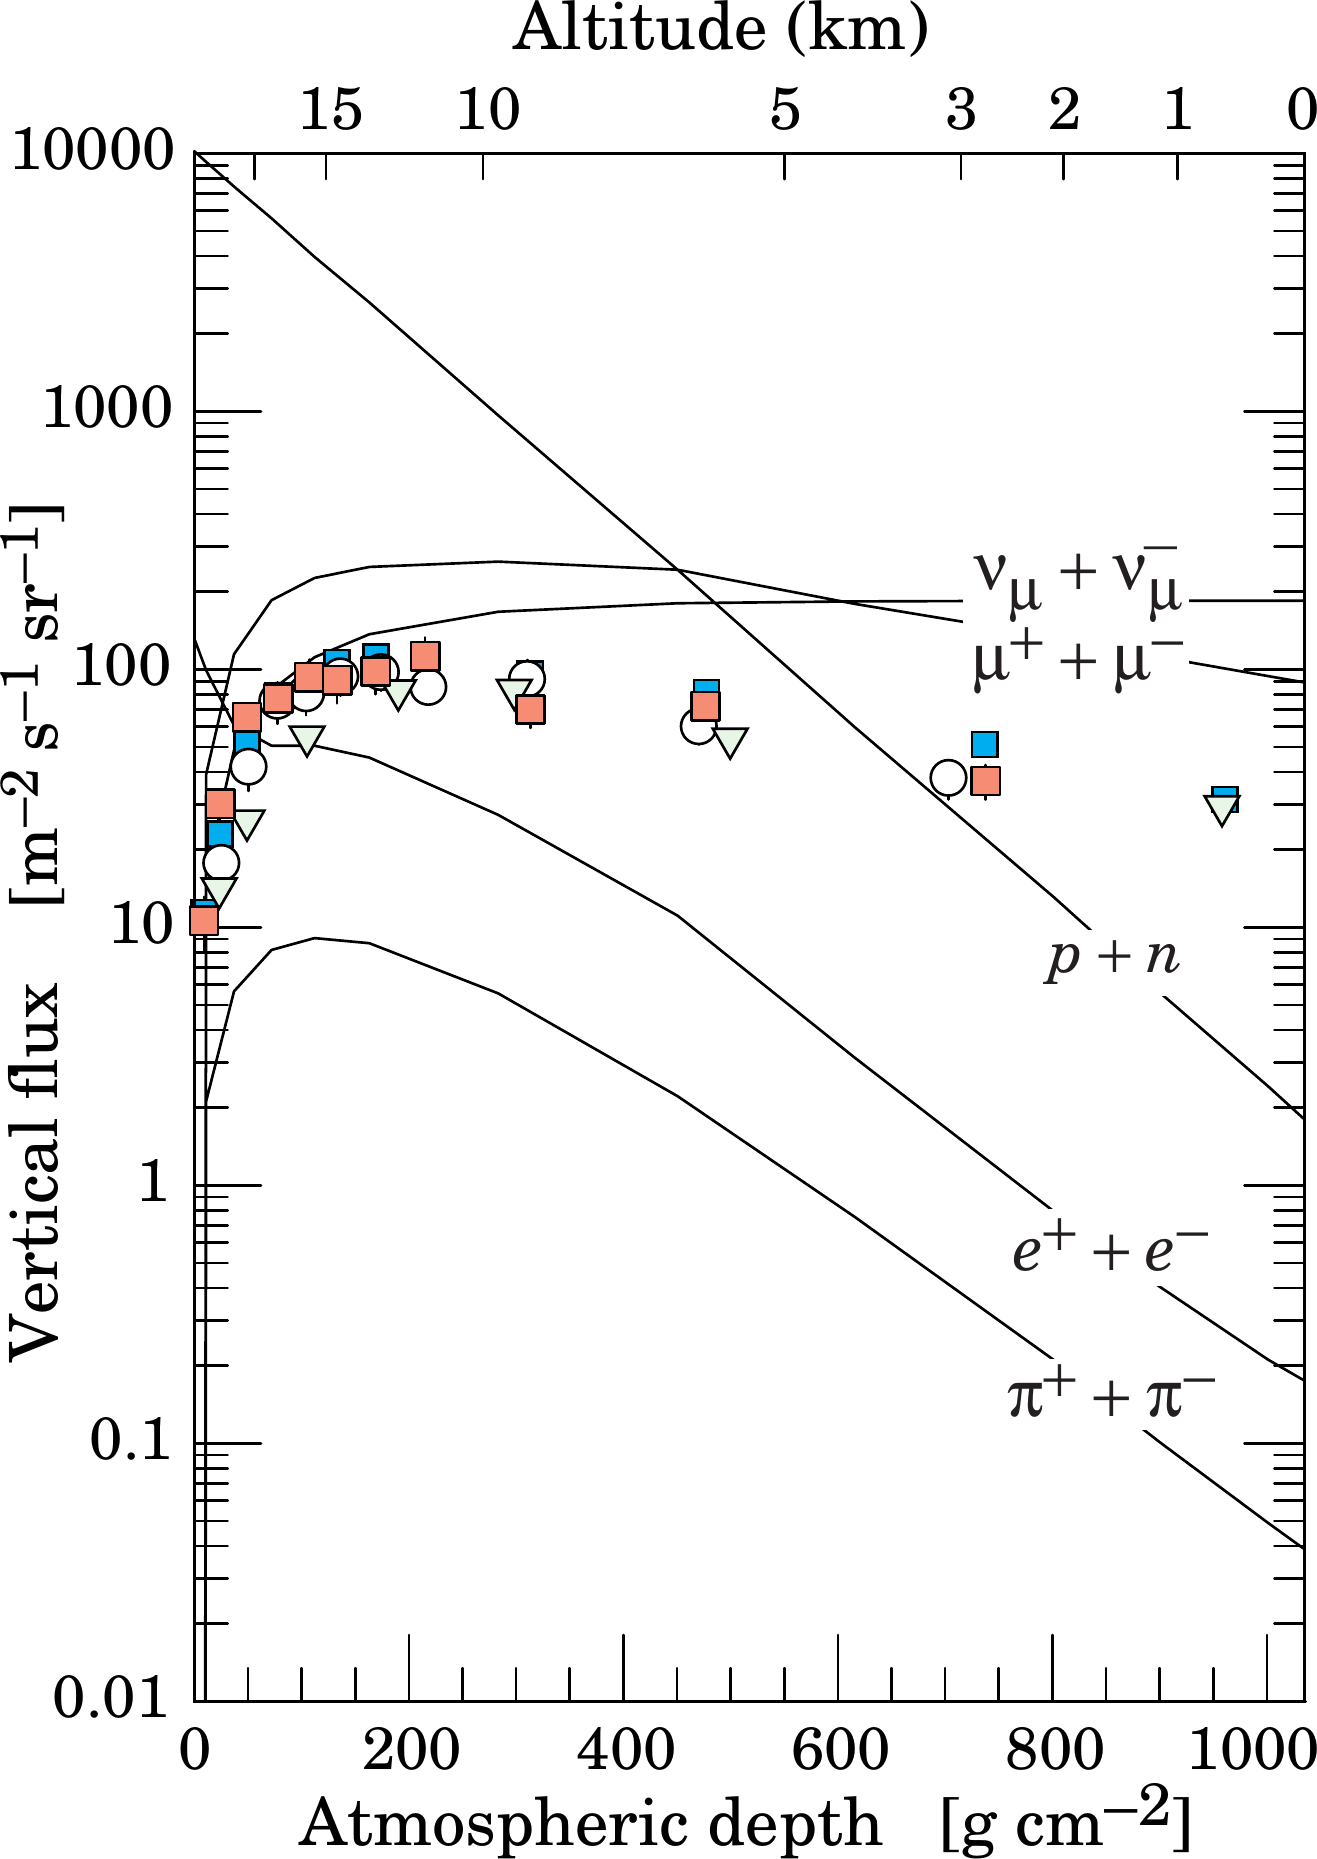
\includegraphics[scale=0.20]{pics/muonflux}
   \caption{Vertical fluxes of cosmic rays in the atmosphere with $E > 1$~GeV estimated %
     from the nucleon flux of Eq.~\ref{eq:cosmicI}. The points show measurements of negative muons %
     with 1 GeV from~ref[32–36].}
   \label{fig:muonflux}
 \end{figure}

 As Fig.~\ref{fig:muonflux} shows, muons are the most numerous charged particles at sea level.
 Muons lose energy to ionisation at a fairly constant rate of about 2~MeV per g/cm$^2$.
 Given taht the vertical depth of the atmosphere is about 1000~g/cm$^2$, muons will lose about two~GeV %
 before reaching the ground. 
 The mean energy of muons at sea level is about four~GeV; therefore the mean energy at creation, %
 tipically fifteen kilometres high, is probably near six~GeV.
 Their energy and angular distribution reflect a convolution of the production spectrum, %
 energy loss in the atmosphere, and decay. 
 The energy spectrum is almost flat below 1 GeV, steepens gradually to reflect the primary %
 spectrum in the 10$\div$100~GeV range, and steepens further at higher energies because pions %
 with $E_\pi > \epsilon_\pi$ tend to interact in the atmosphere before they decay, where %
 $\epsilon_\pi = 115$~GeV is the critical decay energy for pions.
 Asymptotically ($E_\mu \gg $ 1~TeV), the energy spectrum of atmospheric muons is one power %
 steeper than the primary spectrum. 
 The integral intensity of vertical muons above 1~GeV/c at sea level is nearly 70~m$^{-2}$s$^{-1}$sr$^{-1}$ %
 [41,42], with recent measurements [43–45] favoring a lower normalization by 10-15\,\%.
 Another way to express this evaluation is the form 
 \begin{equation}
   \label{eq:muon:rate}
   I_0 \simeq 1~\mathrm{cm^{-2}min^{-1}} = \np{166.7}~\mathrm{m^{-2}Hz}\,,
 \end{equation}
 for horizontal detectors. 
 The overall angular distribution of muons at the ground is $\propto \cos 2\vartheta$, which is %
 characteristic of muons with $E_\mu \sim 3$~GeV. 
% At lower energy the angular distribution becomes increasingly steep, while at higher energy it flattens, %
% approaching a $\sec\vartheta$ distribution for $E_\mu \gg \epsilon_pi$ and $\vartheta < 70^\circ$.
 
 With the beam off, only cosmic rays and background leave a trace in the detector.
 Therefore runs 93 and 94 are useful to characterise the background.

 From Eq.~\ref{eq:ch_Eth}, every muon with an energy $E > \np{159.739}$~MeV can produce Cherenkov %
 radiation, given that the refractive index of water is $n = \np{1.33}$ and %
 the muon mass is \np{105.658}~MeV\footnote{The muon mass is known with an accuaracy of order \np{e-8}. %
   According to the PDF, $m_\mu = \np{105.6583715} \pm \np{0.0000035}$~MeV.}.
 Since the average energy of the muon reaching the ground is well above the Cherenkov thershold, %
 the nominal flux at sea level can be used to evaluate the cosmic background rate.
 The water tank is placed eight meters below the surface, and it fits the hall's walls, hence only the top %
 area of the tank (slightly more than 7~m$^2$) could be taken in consideration.
 A rough estimation would suggest that the number of muons reaching the detector is 
 \begin{equation}
   \label{eq:anniemuon}
   I \simeq 7\,I_0~\mathrm{m^2} \simeq \np{1178.1}~Hz\,.
 \end{equation}

\section{Threshold dependance}

Three parameters of the Data Analysis software have been tuned so as to study the feedback %
of the rejection method.
The parameters are:
\begin{enumerate}
  \item Voltage threshold;
  \item Number of PMTs fired;
  \item Time rejection window.
\end{enumerate}

\subsection{Voltage}
\subsection{PMTs fired}
\subsection{Rejection window}

\section{Michel decay}
I've seen it, it could be a nice plot to place here. 

\section{Neutron yield}
No luck yet.
really not sure about this section.

\section{First MRD data}
TDC, could do some dummy analysis.

%%%%%%%%%%%%%%%%%%%%%%%%%%%%%%%		CHAP 6		%%%%%%%%%%%%%%%%%%%%%%%%%%%%%%%

\chapter{Conclusions}
\label{cha:6}


\appendix
%%%%%%%%%%%%%%%%%%%%%%%%%%%%%%%		APP		%%%%%%%%%%%%%%%%%%%%%%%%%%%%%%%

\chapter{Booster Neutrino Beam}
\label{app:A}

 %Arxiv 1311.5958v1.
 %Fermilab has two major neutrino beamlines: the Neutrino Main Injector (NuMI) and %
 %the Booster Neutrino Beam (BNB).
 %The energy range of these two neutrino sources on-axis is in the GeV range, %
 %which is too high to satisfy the condition for dominance of coherent scattering. 
 %The far-off-axis (> $45^\circ$) of the BNB produces well defined neutrinos with %
 %energies below 50 MeV.
 %The BNB source has substantial advantages over the NuMI beam source owing to suppressed %
 %kaon production from the relatively low energy 8 GeV proton beam on the target~ref. 
 %Therefore, pion decay and subsequent muon decay processes are the dominant sources of neutrinos. 
 %At the far-off-axis area, the detector can be placed close enough to the target to gain a %
 %large increase in neutrino flux due to the larger solid angle acceptance.

 \section{BNB details}
 %An initial study using the existing BNB MC has confirmed that this approach is promising.
 %The Fermilab Booster is a 474-meter-circumference synchrotron operating at 15 Hz. 
 %Protons from the Fermilab LINAC are injected at 400 MeV and accelerated to 8 GeV kinetic energy. 
 %The structure of the beam is a series of 81 proton bunches each with a 2 ns width and 19 ns apart. 
 %The maximum average repetition rate for proton delivery to the BNB is 5 Hz and 5 x 10 12 protons %
 %per pulse. 
 %The repetition limit is set by the horn design and its power supply. 
 %The target is made of beryllium divided in seven cylindrical sections in a total of \np{71.1}~cm %
 %in length and 0.51 cm in radius.
 %In order to minimize up-stream proton interactions, the vacuum of the beam pipe extends to %
 %about 152 cm upstream of the target.
 %The horn is an aluminum alloy toroidal electromagnet with operating values of 174 kA and %
 %maximum field value of 1.5 Tesla. 
 %A concrete collimator is located downstream of the target and guides the beam into the decay region.
 %The air-filled cylindrical decay region extends for 45 meters. 
 %The beam stop is made of steel and concrete. 
 
 %PHYSICAL REVIEW D 79, 072002 (2009).
 %The Fermi National Accelerator Laboratory (FNAL) booster is a 474-meter-circumference %
 %synchrotron operating at 15 Hz. 
 %Protons from the Fermilab LINAC are injected at 400 MeV and accelerated to 8 GeV kinetic %
 %energy (8:89 GeV=c momentum).
 %he booster has a harmonic number of 84, of which 81 buckets are filled. 
 %Thebeam is extracted into the BNB using a fast-rising kicker that extracts all of the particles %
 %in a single turn.
 %The resulting structure is a series of 81 bunches of protons each 2 ns wide and 19 ns apart.
 %Upon leaving the booster, the proton beam is transported through a lattice of focusing %
 %and defocusing quadrupole (FODO) and dipole magnets.
 %A switch magnet steers the beam to the main injector or to the BNB. 
 %The BNB is also a FODO that terminates with a triplet that focuses the beamon the target. 
 %The design and measured optics of BNB are in agreement [7,8].
 %The maximum allowable average repetition rate for delivery of protons to the BNB is %
 %5 Hz (with a maximumof 11 pulses in a row at 15 Hz) and 5 x 10to12 protons-per-pulse. 
 %The 5 Hz limit is set by the design of the horn (described below) and its power supply.
 
 %The target consists of seven identical cylindrical slugs of beryllium arranged to produce a %
 %cylinder 71.1 cm long and 0.51 cm in radius. 
 %The target is contained within a beryllium sleeve 0.9 cm thick with an inner radius of 1.37 cm.
 %Each target slug is supported within the sleeve by three ``fins'' (also beryllium) %
 %which extend radially out from the target to the sleeve. 
 %The volume of air within the sleeve is circulated to provide cooling for the target when the beam %
 %line is in operation. 
 %The target and associated assembly are shown in Fig.~2, where the top figure shows an exploded %
 %view of the various components (with the downstream end of the target on the right), %
 %and the bottom shows the components in assembled form. 
 %The choice of beryllium as the target material was motivated by residual radioactivity issues %
 %in the event that the target assembly needed to be replaced, as well as energy loss %
 %considerations that allow the air-cooling system to be sufficient.
 %Upstream of the target, the primary proton beam is monitored using four systems: %
 %two toroids measuring its intensity (protons-per-pulse), beam position monitors %
 %(BPM) and a multiwire chamber determining the beam width and position, %
 %and a resistive wall monitor (RWM) measuring both the time and intensity of the beam spills.
 %The vacuum of the beam pipe extends to about 5 feet upstream of the target, %
 %minimizing upstream proton interactions.
 %The toroids are continuously calibrated at 5 Hz with their absolute calibrations verified %
 %twice a year.
 %The calibrations have shown minimal deviation ( < 0:5\%).
 %The proton flux measured in the two toroids agree to within 2\%, compatible with the %
 %expected systematic uncertainties.
 %The BPMs are split-plate devices that measure the difference of charge induced on two plates. 
 %By measuring the change in beam position at several locations without intervening optics, %
 %the BPMs are found to be accurate to 0.1 mm (standard deviation). 
 %The multiwire is a wire chamber with 48 horizontal and 48 vertical wires and 0.5 mm pitch. 
 %The profile of the beam is measured using the secondary emission induced by the beam on the wires.
 %The RWM is located upstream of the target to monitor the time and intensity of the proton %
 %pulses prior to striking the target. 
 %While the data from the RWM did not directly entere analysis, it allowed many useful cross %
 %checks, such as those shown in Fig. 3.
 %The left figure shows a comparison of the production times of neutrinos observed %
 %in the MiniBooNE detector estimated based on the vertex and time reconstructed by the detector %
 %and subtracting the time-of-flight. 
 %This time is then compared to the nearest bucket as measured by the RWM. 
 %The distribution indicates that neutrino events can be matched not only to pulses %
 %from the booster, but to a specific bucket within the pulse.
 %The tails of the distribution result from the resolution of the vertex reconstruction %
 %of the neutrino event in the detector, which is needed to determine the time of the %
 %event and correct for the time-of-flight.
 %The right plot demonstrates the synchronization of the horn pulse (described in Sec. II C) %
 %with the delivery of the beam as measured by the RWM.
 
 %The horn current pulse is approximately a half-sinusoid of amplitude 174 kA, 143 s long, %
 %synchronized to each beam spill. 
 
 %The typical beam alignment and divergence measured by the beam position monitors located %
 %near the target are within 1 mm and 1 mrad of the nominal target center and axis direction, %
 %respectively; the typical beam focusing on target measured by beam profile monitors is %
 %of the order of 1–2 mm [root mean square(RMS)] in both the horizontal and vertical directions.
 %These parameters are well within the experiment requirements. 
 %The number of protons delivered to the BNB target is measured for each proton %
 %batch using two toroids located near the target along the beam line. 
 %The toroid calibration, performed on a pulse-by-pulse basis, provides a measurement %
 %of the number of protons to BNB with a 2\,\% accuracy.
 %Primary protons from the 8 GeV beam line strike a thick beryllium target located %
 %in the BNB target hall.
 
 %The SciBooNE hall is on axis from the Booster Neutrino Beam (BNB) at 8 m below the surface.
 %The BNB impinges 8.89 GeV/c protons from the booster on a beryllium target, with %
 %4 x10to12 delivered in a narrow spill of approximately 1.6 micros at a frequency of 7.5 Hz. 
 %The projected number of protons incident on the target (POT) per year for the BNB is %
 %about 2 x 10to 20 POT.
 %The rates expected per year when running in neutrino mode for 1 ton of water %
 %(the approximate usable fiducial volume) are about 16K neutrino interactions, %
 %where 11K of those would be numu CC interactions. 
 %This spectrum peaks ideally in the region of interest at 700 MeV as shown left of Figure 2 %
 %and has the target rate of neutrino interactions per year.
 %The spectrum and rates are based on BNB flux simulated data provided by Zarko Pavlovic (FNAL)%
 %appropriately propagated to the SciBoone hall.
 
 %The target is made of seven cylindrical slugs for a total target length of 71.1 cm, %
 %or about 1.7 inelastic interaction lengths.
 %The beryllium target is surrounded by a magnetic focusing horn, bending and %
 %sign-selecting the secondary particles that emerge from the interactions in the target along
 %the direction pointing to the SciBooNE detector.
 %The focusing is produced by the toroidal magnetic field present in the air volume %
 %between the horn’s two coaxial conductors made of aluminum alloy. 
 %The horn current pulse is approximately a half-sinusoid of amplitude 174 kA, 143 s long, %
 %synchronized to each beam spill. 
 %The polarity of the horn current flow can be (and has been) switched, in order to %
 %focus negatively charged mesons, and therefore produce an antineutrino instead of a neutrino beam.
 %The beam of focused, secondary mesons emerging from the target/horn region is further collimated, %
 %via passive shielding, and allowed to decay into neutrinos in a cylindrical decay %
 %region filled with air at atmospheric pressure, 50 m long and 90 cm in radius. 
 %A beam absorber located at the end of the decay region stops the hadronic and muonic %
 %component of the beam, and only a pure neutrino beam pointing toward the detector remains, %
 %mostly from a pion to mu+ nuofmu decays.



 \section{Resistive Wall Monitor}
 %A resistive wall monitor measures the image charge that flows along the vacuum %
 %chamber following the beam. The image charge has equal magnitude but opposite sign.
 %Depending on the beam velocity, the image charge will lag behind and be spread out along its path. 
 %The ultimate bandwidth of such a detector is limited by this spreading of %
 %the electric field lines between the beam and the inside walls of the beam pipe.
 %The spreading angle is approximately 1/ gamma for relativistic beams ( gamma is the ratio %
 %of total energy to rest energy). 
 %The estimated bandwidth limit from spreading is 47 GHz at injection to the Main Injector %
 %for a 3 cm radius pipe and 8 GeV proton energy. 
 %In practice, the detector response is difficult to maintain above the microwave cutoff %
 %frequency of the beam pipe,measured to be 1.5 GHz for the elliptical beam pipe used in %
 %the Main Injector. 
 %Above cutoff, the characteristic impedance of the beam pipe and the impedance of nearby %
 %structures such as bellows or changes in geometry can effect accuracy.
 
 %In order to measure the image current, the beam pipe is cut and a resistive gap is %
 %inserted (Figure 1). 
 %Various ferrite cores are used to force the image current through the resistive gap rather %
 %than allowing it to flow through other conducting paths.
 %In addition to image current, other currents are often found flowing along the beam pipe. 
 %The gap and cores are placed inside a metal can to shunt these “noise” currents around %
 %rather than through the resistive gap. 
 %The inductance of the cores and the resistance of the gap forms a high pass filter with %
 %a corner frequency of R/2piL, typically a few kilohertz.
 %Above this frequency, cores act to minimize the net current through their center %
 %by inducing a current through the resistive gap that just cancels the beam current.
 %The gap impedance is chosen to be well below the impedance of the cores inside the shielding can. %
 %Several types of ferrite and microwave absorbers are used to maximize the impedance and %
 %minimize resonances within the desired bandwidth. 
 %The Main Injector shielding can has an impedance greater than 30 ohms with the ferrite cores. 
 %In parallel with the 1 ohm gap impedance, 30 ohms can cause frequency dependent errors %
 %of pm1.5\% or 0.15 db.
 %If the charge density around the circumference of the gap is not uniform, the voltage %
 %across the gap will vary around the circumference. 
 %The gap will act as an azimuthal transmission line transporting charge until the %
 %voltage equalizes. 
 %The time domainresponse of the detector would be distorted during this time. 
 %Position detectors have been made by exploiting this effect. 
 %The elliptical shape of the Main Injector pipe aggravates this problem (Figure 2). 
 %To overcome this problem, a round geometry is used for the gap and the signals from %
 %several monitor points equally spaced around the circumference are combined to form a single output. 

%%%%%%%%%%%%%%%%%%%%%%%%%%%%%%%		APP		%%%%%%%%%%%%%%%%%%%%%%%%%%%%%%%

\chapter{Booster Neutrino Beam}
\label{app:B}


ANNIE is run off the Booster Neutrino Beam in Fermilab.
Fermilab Booster accelerates the protons up to 8 GeV kinetic energy.
Selected spills containing approximately 4-5x10 12 protons are extracted and %
bent toward the BNB target hall.
Each spill contains 81 bunches of protons, approximately 6 nsec wide each and 19 nsec apart, %
for a total spill duration of 1.6 usec.
The typical beam alignment and divergence, measured by the beam position %
monitors located near the target, are within 1 mm and 1 mrad of the nominal target center %
and axis direction, respectively.
The typical beam focusing on target measured by the beam profile monitors is of the order %
of 1-2 mm (RMS) in both the horizontal and vertical directions.
The number of protons delivered to the BNB target for each spill is measured with a %
2\% accuracy using two toroidal current transformers (often referred to as toroid’s) %
located near the target along the beamline.
These parameters are well tuned within the experiment requirements.



%%%%%%%%%%%%%%%%%%%%%%%%%%%%%%%%%%%%%%%%%%%%		APP		%%%%%%%%%%%%%%%%%%%%%%%%%%%%%%%%%%%%%%%%%%%%

 \subsectionfont{\LARGE \centering}

 \chapter{Fit results}
 \label{app:C}
  
 In this appendix, the fit result mentioned in section~\ref{sec:muon} are reported in their entirety.

 \section{Event}

 The behaviour of the event spectrum is exponential, thereby the following function was fitted:
 \begin{equation}
   y = N \mathrm{e}^{-x / \tau} + c_E \,.
 \end{equation}

 \subsection*{$C$}

 \begin{minipage}[c][3cm][t]{0.5\textwidth}
  \centering
  Correlation matrix
 \[
   \begin{array}{crrrr}
   \toprule
      		& N		&1/\tau		& c_E		& \text{Global}	\\
   \midrule
   N		& \np{1.000}	& \np{-0.996}	& \np{0.532}	& \np{0.997}	\\
   1/\tau	& \np{-0.996} 	& \np{ 1.000}	& \np{-0.563}	& \np{0.997}	\\ 
   c_E		& \np{0.532}	& \np{-0.563}	& \np{1.000}	& \np{0.650}	\\ 
   \bottomrule
  \end{array}
 \]
 \end{minipage}
 \begin{minipage}[c][3cm][t]{0.5\textwidth}
   \centering
   Best fit
 \[
   \begin{array}{crrrc}
   \toprule
		& \text{Value}	& \text{Error}	& \text{Err} \%	& \text{Unit}	\\
   \midrule                                                     
   N		& \np{12.43}	& \np{0.09}	&		& 	\\
   1/\tau	& \np{-0.340} 	& \np{0.007}	&		& \mu\mathrm{s}^{-1}	\\ 
   c_E		& \np{5756}	& \np{8}	&		& 	\\ 
   \bottomrule
  \end{array}
 \]
 \end{minipage}

 \subsection*{$V_{00}$}
 \begin{minipage}[c][3cm][t]{0.5\textwidth}
  \centering
  Correlation matrix
 \[
   \begin{array}{crrrr}
   \toprule
      		& N		&1/\tau		& c_E		& \text{Global}	\\
   \midrule
   N		& \np{1.000}	& \np{-0.989}	& \np{0.508}	& \np{0.991}	\\
   1/\tau	& \np{-0.989} 	& \np{ 1.000}	& \np{-0.568}	& \np{0.992}	\\ 
   c_E		& \np{0.508}	& \np{-0.568}	& \np{1.000}	& \np{0.674}	\\ 
   \bottomrule
  \end{array}
 \]
 \end{minipage}
 \begin{minipage}[c][3cm][t]{0.5\textwidth}
   \centering
   Best fit
 \[
   \begin{array}{crrrc}
   \toprule
		& \text{Value}	& \text{Error}	& \text{Err} \%	& \text{Unit}	\\
   \midrule                                                     
   N		& \np{12.43}	& \np{0.03}	&		& 	\\
   1/\tau	& \np{-0.340} 	& \np{0.002}	&		& \mu\mathrm{s}^{-1}	\\ 
   c_E		& \np{10.18e3}	& \np{0.01e3}	&		& 	\\ 
   \bottomrule
  \end{array}
 \]
 \end{minipage}

 \subsection*{$V_{01}$}
 \begin{minipage}[c][3cm][t]{0.5\textwidth}
  \centering
  Correlation matrix
 \[
   \begin{array}{crrrr}
   \toprule
      		& N		&1/\tau		& c_E		& \text{Global}	\\
   \midrule
   N		& \np{1.000}	& \np{-0.990}	& \np{0.446}	& \np{0.992}	\\
   1/\tau	& \np{-0.990} 	& \np{ 1.000}	& \np{-0.518}	& \np{0.992}	\\ 
   c_E		& \np{0.446}	& \np{-0.518}	& \np{1.000}	& \np{0.620}	\\ 
   \bottomrule
  \end{array}
 \]
 \end{minipage}
 \begin{minipage}[c][3cm][t]{0.5\textwidth}
   \centering
   Best fit
 \[
   \begin{array}{crrrc}
   \toprule
		& \text{Value}	& \text{Error}	& \text{Err} \%	& \text{Unit}	\\
   \midrule                                                     
   N		& \np{12.05}	& \np{0.03}	&		& 	\\
   1/\tau	& \np{-0.249} 	& \np{0.002}	&		& \mu\mathrm{s}^{-1}	\\ 
   c_E		& \np{8701}	& \np{9}	&		& 	\\ 
   \bottomrule
  \end{array}
 \]
 \end{minipage}

 \subsection*{$V_{05}$}
 \begin{minipage}[c][3cm][t]{0.5\textwidth}
  \centering
  Correlation matrix
 \[
   \begin{array}{crrrr}
   \toprule
      		& N		&1/\tau		& c_E		& \text{Global}	\\
   \midrule
   N		& \np{1.000}	& \np{-0.996}	& \np{0.434}	& \np{0.997}	\\
   1/\tau	& \np{-0.996} 	& \np{ 1.000}	& \np{-0.462}	& \np{0.997}	\\ 
   c_E		& \np{0.434}	& \np{-0.462}	& \np{1.000}	& \np{0.554}	\\ 
   \bottomrule
  \end{array}
 \]
 \end{minipage}
 \begin{minipage}[c][3cm][t]{0.5\textwidth}
   \centering
   Best fit
 \[
   \begin{array}{crrrc}
   \toprule
		& \text{Value}	& \text{Error}	& \text{Err} \%	& \text{Unit}	\\
   \midrule                                                     
   N		& \np{11.4}	& \np{0.2}	&		& 	\\
   1/\tau	& \np{-0.36} 	& \np{0.02}	&		& \mu\mathrm{s}^{-1}	\\ 
   c_E		& \np{3594}	& \np{5}	&		& 	\\ 
   \bottomrule
  \end{array}
 \]
 \end{minipage}

 \subsection*{$V_{10}$}
 \begin{minipage}[c][3cm][t]{0.5\textwidth}
  \centering
  Correlation matrix
 \[
   \begin{array}{crrrr}
   \toprule
      		& N		&1/\tau		& c_E		& \text{Global}	\\
   \midrule
   N		& \np{1.000}	& \np{-0.858}	& \np{0.709}	& \np{0.963}	\\
   1/\tau	& \np{-0.858} 	& \np{ 1.000}	& \np{-0.963}	& \np{0.995}	\\ 
   c_E		& \np{0.709}	& \np{-0.963}	& \np{1.000}	& \np{0.990}	\\ 
   \bottomrule
  \end{array}
 \]
 \end{minipage}
 \begin{minipage}[c][3cm][t]{0.5\textwidth}
   \centering
   Best fit
 \[
   \begin{array}{crrrc}
   \toprule
		& \text{Value}	& \text{Error}	& \text{Err} \%	& \text{Unit}	\\
   \midrule                                                     
   N		& \np{6.0}	& \np{0.1}	&		& 	\\
   1/\tau	& \np{-0.46} 	& \np{0.01}	&		& \mu\mathrm{s}^{-1}	\\ 
   c_E		& \np{2.57e3}	& \np{0.02e3}	&		& 	\\ 
   \bottomrule
  \end{array}
 \]
 \end{minipage}

 \subsection*{$N_{15}$}
 \begin{minipage}[c][3cm][t]{0.5\textwidth}
  \centering
  Correlation matrix
 \[
   \begin{array}{crrrr}
   \toprule
      		& N		&1/\tau		& c_E		& \text{Global}	\\
   \midrule
   N		& \np{1.000}	& \np{-0.997}	& \np{0.539}	& \np{0.997}	\\
   1/\tau	& \np{-0.997} 	& \np{ 1.000}	& \np{-0.567}	& \np{0.997}	\\ 
   c_E		& \np{0.539}	& \np{-0.567}	& \np{1.000}	& \np{0.645}	\\ 
   \bottomrule
  \end{array}
 \]
 \end{minipage}
 \begin{minipage}[c][3cm][t]{0.5\textwidth}
   \centering
   Best fit
 \[
   \begin{array}{crrrc}
   \toprule
		& \text{Value}	& \text{Error}	& \text{Err} \%	&\text{Unit}	\\
   \midrule
   N		& \np{12.2}	& \np{0.1}	&		& 	\\
   1/\tau	& \np{-0.327} 	& \np{0.008}	&		& \mu\mathrm{s}^{-1}	\\ 
   c_E		& \np{5488}	& \np{7}	&		& 	\\ 
   \bottomrule
  \end{array}
 \]
 \end{minipage}

 \subsection*{$N_{30}$}
 \begin{minipage}[c][3cm][t]{0.5\textwidth}
  \centering
  Correlation matrix
 \[
   \begin{array}{crrrr}
   \toprule
      		& N		&1/\tau		& c_E		& \text{Global}	\\
   \midrule
   N		& \np{1.000}	& \np{-0.996}	& \np{0.560}	& \np{0.997}	\\
   1/\tau	& \np{-0.996} 	& \np{ 1.000}	& \np{-0.562}	& \np{0.997}	\\ 
   c_E		& \np{0.560}	& \np{-0.592}	& \np{1.000}	& \np{0.680}	\\ 
   \bottomrule
  \end{array}
 \]
 \end{minipage}
 \begin{minipage}[c][3cm][t]{0.5\textwidth}
   \centering
   Best fit
 \[
   \begin{array}{crrrc}
   \toprule
		& \text{Value}	& \text{Error}	& \text{Err} \%	&\text{Unit}	\\
   \midrule
   N		& \np{11.8}	& \np{0.1}	&		& 	\\
   1/\tau	& \np{-0.326} 	& \np{0.01}	&		& \mu\mathrm{s}^{-1}	\\ 
   c_E		& \np{5103}	& \np{8}	&		& 	\\ 
   \bottomrule
  \end{array}
 \]
 \end{minipage}

 \subsection*{$N_{50}$}
 \begin{minipage}[c][3cm][t]{0.5\textwidth}
  \centering
  Correlation matrix
 \[
   \begin{array}{crrrr}
   \toprule
      		& N		&1/\tau		& c_E		& \text{Global}	\\
   \midrule
   N		& \np{1.000}	& \np{-0.996}	& \np{0.497}	& \np{0.996}	\\
   1/\tau	& \np{-0.996} 	& \np{ 1.000}	& \np{-0.527}	& \np{0.997}	\\ 
   c_E		& \np{0.497}	& \np{-0.527}	& \np{1.000}	& \np{0.610}	\\ 
   \bottomrule
  \end{array}
 \]
 \end{minipage}
 \begin{minipage}[c][3cm][t]{0.5\textwidth}
   \centering
   Best fit
 \[
   \begin{array}{crrrc}
   \toprule
		& \text{Value}	& \text{Error}	& \text{Err} \%	&\text{Unit}	\\
   \midrule
   N		& \np{11.1}	& \np{0.1}	&		& 	\\
   1/\tau	& \np{-0.30} 	& \np{0.01}	&		& \mu\mathrm{s}^{-1}	\\ 
   c_E		& \np{4085}	& \np{5}	&		& 	\\ 
   \bottomrule
  \end{array}
 \]
 \end{minipage}

 \subsection*{$\Delta_{50}$}
 \begin{minipage}[c][3cm][t]{0.5\textwidth}
  \centering
  Correlation matrix
 \[
   \begin{array}{crrrr}
   \toprule
      		& N		&1/\tau		& c_E		& \text{Global}	\\
   \midrule
   N		& \np{1.000}	& \np{-0.997}	& \np{0.406}	& \np{0.997}	\\
   1/\tau	& \np{-0.997} 	& \np{ 1.000}	& \np{-0.427}	& \np{0.998}	\\ 
   c_E		& \np{0.406}	& \np{-0.427}	& \np{1.000}	& \np{0.499}	\\ 
   \bottomrule
  \end{array}
 \]
 \end{minipage}
 \begin{minipage}[c][3cm][t]{0.5\textwidth}
   \centering
   Best fit
 \[
   \begin{array}{crrrc}
   \toprule
		& \text{Value}	& \text{Error}	& \text{Err} \%	&\text{Unit}	\\
   \midrule
   N		& \np{11.35}	& \np{0.08}	&		& 	\\
   1/\tau	& \np{-0.403} 	& \np{0.006}	&		& \mu\mathrm{s}^{-1}	\\ 
   c_E		& \np{6055}	& \np{6}	&		& 	\\ 
   \bottomrule
  \end{array}
 \]
 \end{minipage}

 \subsection*{$\Delta_{30}$}
 \begin{minipage}[c][3cm][t]{0.5\textwidth}
  \centering
  Correlation matrix
 \[
   \begin{array}{crrrr}
   \toprule
      		& N		&1/\tau		& c_E		& \text{Global}	\\
   \midrule
   N		& \np{1.000}	& \np{-0.999}	& \np{0.620}	& \np{0.999}	\\
   1/\tau	& \np{-0.999} 	& \np{ 1.000}	& \np{-0.633}	& \np{0.999}	\\ 
   c_E		& \np{0.620}	& \np{-0.633}	& \np{1.000}	& \np{0.682}	\\ 
   \bottomrule
  \end{array}
 \]
 \end{minipage}
 \begin{minipage}[c][3cm][t]{0.5\textwidth}
   \centering
   Best fit
 \[
   \begin{array}{crrrc}
   \toprule
		& \text{Value}	& \text{Error}	& \text{Err} \%	&\text{Unit}	\\
   \midrule
   N		& \np{12.9}	& \np{0.2}	&		& 	\\
   1/\tau	& \np{-0.38} 	& \np{0.01}	&		& \mu\mathrm{s}^{-1}	\\ 
   c_E		& \np{5337}	& \np{7}	&		& 	\\ 
   \bottomrule
  \end{array}
 \]
 \end{minipage}

 \subsection*{$\Delta_{20}$}
 \begin{minipage}[c][3cm][t]{0.5\textwidth}
  \centering
  Correlation matrix
 \[
   \begin{array}{crrrr}
   \toprule
      		& N		&1/\tau		& c_E		& \text{Global}	\\
   \midrule
   N		& \np{1.000}	& \np{-0.998}	& \np{0.394}	& \np{0.998}	\\
   1/\tau	& \np{-0.998} 	& \np{ 1.000}	& \np{-0.409}	& \np{0.998}	\\ 
   c_E		& \np{0.394}	& \np{-0.409}	& \np{1.000}	& \np{0.473}	\\ 
   \bottomrule
  \end{array}
 \]
 \end{minipage}
 \begin{minipage}[c][3cm][t]{0.5\textwidth}
   \centering
   Best fit
 \[
   \begin{array}{crrrc}
   \toprule
		& \text{Value}	& \text{Error}	& \text{Err} \%	&\text{Unit}	\\
   \midrule
   N		& \np{14.1}	& \np{0.1}	&		& 	\\
   1/\tau	& \np{-0.48} 	& \np{0.01}	&		& \mu\mathrm{s}^{-1}	\\ 
   c_E		& \np{4295}	& \np{5}	&		& 	\\ 
   \bottomrule
  \end{array}
 \]
 \end{minipage}

 \subsection*{$\Delta_{10}$}
 \begin{minipage}[c][3cm][t]{0.5\textwidth}
  \centering
  Correlation matrix
 \[
   \begin{array}{crrrr}
   \toprule
      		& N		&1/\tau		& c_E		& \text{Global}	\\
   \midrule
   N		& \np{1.000}	& \np{-0.998}	& \np{0.335}	& \np{0.998}	\\
   1/\tau	& \np{-0.998} 	& \np{ 1.000}	& \np{-0.352}	& \np{0.998}	\\ 
   c_E		& \np{0.335}	& \np{-0.352}	& \np{1.000}	& \np{0.424}	\\ 
   \bottomrule
  \end{array}
 \]
 \end{minipage}
 \begin{minipage}[c][3cm][t]{0.5\textwidth}
   \centering
   Best fit
 \[
   \begin{array}{crrrc}
   \toprule
		& \text{Value}	& \text{Error}	& \text{Err} \%	&\text{Unit}	\\
   \midrule
   N		& \np{13.6}	& \np{0.2}	&		& 	\\
   1/\tau	& \np{-0.48} 	& \np{0.01}	&		& \mu\mathrm{s}^{-1}	\\ 
   c_E		& \np{3346}	& \np{4}	&		& 	\\ 
   \bottomrule
  \end{array}
 \]
 \end{minipage}

 \section{Noise}

 The behaviour of the event spectrum is exponential, thereby the following function was fitted:
 \begin{equation}
   y = A \exp{\bigg (-\frac{(x-\mu)^2}{2\sigma^2} \bigg )} + c_N\,.
 \end{equation}

 \subsection*{$C$}
 \begin{center}
  Correlation matrix
 \[
   \begin{array}{crrrrr}
   \toprule
      		& A		& \mu		& \sigma	& c_N		& \text{Global}	\\
   \midrule
   A		& \np{1.000}	& \np{0.170}	& \np{0.574}	& \np{-0.150}	& \np{0.694}	\\
   \mu		& \np{0.170} 	& \np{1.000}	& \np{0.321}	& \np{0.010}	& \np{0.350}	\\ 
   \sigma	& \np{0.574}	& \np{0.321}	& \np{1.000}	& \np{0.364}	& \np{0.762}	\\ 
   c_N		& \np{-0.150}	& \np{0.010}	& \np{0.364}	& \np{1.000}	& \np{0.582}	\\ 
   \bottomrule
  \end{array}
 \]
   Best fit
 \[
   \begin{array}{crrrc}
   \toprule
		& \text{Value}	& \text{Error}	& \text{Err} \%	& \text{Unit}	\\
   \midrule                                                     
   A		& \np{1.43e3}	& \np{0.03e3}	&		& 	\\
   \mu		& \np{17.66} 	& \np{0.05}	&		& \mu\mathrm{s}	\\ 
   \sigma	& \np{2.03}	& \np{0.07}	&		& \mu\mathrm{s}	\\ 
   c_N		& \np{6312}	& \np{9}	&		& 	\\ 
   \bottomrule
  \end{array}
 \]
 \end{center}

 \subsection*{$V_{00}$}
 \begin{center}
  Correlation matrix
 \[
   \begin{array}{crrrrr}
   \toprule
      		& A		& \mu		& \sigma	& c_N		& \text{Global}	\\
   \midrule
   A		& \np{1.000}	& \np{0.038}	& \np{-0.615}	& \np{-0.078}	& \np{0.726}	\\
   \mu		& \np{0.038} 	& \np{1.000}	& \np{-0.062}	& \np{-0.064}	& \np{0.131}	\\ 
   \sigma	& \np{-0.615}	& \np{-0.062}	& \np{1.000}	& \np{-0.435}	& \np{0.786}	\\ 
   c_N		& \np{-0.078}	& \np{-0.064}	& \np{-0.435}	& \np{1.000}	& \np{0.625}	\\ 
   \bottomrule
  \end{array}
 \]
   Best fit
 \[
   \begin{array}{crrrc}
   \toprule
		& \text{Value}	& \text{Error}	& \text{Err} \%	& \text{Unit}	\\
   \midrule                                                     
   A		& \np{4.16e3}	& \np{0.06e3}	&		& 	\\
   \mu		& \np{17.85} 	& \np{0.03}	&		& \mu\mathrm{s}	\\ 
   \sigma	& \np{2.24}	& \np{0.06}	&		& \mu\mathrm{s}	\\ 
   c_N		& \np{29.87e3}	& \np{0.02e3}	&		& 	\\ 
   \bottomrule
  \end{array}
 \]
 \end{center}

 \subsection*{$V_{01}$}
 \begin{center}
  Correlation matrix
 \[
   \begin{array}{crrrrr}
   \toprule
      		& A		& \mu		& \sigma	& c_N		& \text{Global}	\\
   \midrule
   A		& \np{1.000}	& \np{0.082}	& \np{-0.670}	& \np{-0.030}	& \np{0.744}	\\
   \mu		& \np{0.082} 	& \np{1.000}	& \np{-0.154}	& \np{-0.031}	& \np{0.200}	\\ 
   \sigma	& \np{-0.670}	& \np{-0.154}	& \np{1.000}	& \np{-0.391}	& \np{0.794}	\\ 
   c_N		& \np{-0.030}	& \np{-0.031}	& \np{-0.391}	& \np{1.000}	& \np{0.565}	\\ 
   \bottomrule
  \end{array}
 \]
   Best fit
 \[
   \begin{array}{crrrc}
   \toprule
		& \text{Value}	& \text{Error}	& \text{Err} \%	& \text{Unit}	\\
   \midrule                                                     
   A		& \np{3.53e3}	& \np{0.05e3}	&		& 	\\
   \mu		& \np{17.73} 	& \np{0.03}	&		& \mu\mathrm{s}	\\ 
   \sigma	& \np{2.18}	& \np{0.06}	&		& \mu\mathrm{s}	\\ 
   c_N		& \np{29.84e3}	& \np{0.01e3}	&		& 	\\ 
   \bottomrule
  \end{array}
 \]
 \end{center}

 \subsection*{$V_{05}$}
 \begin{center}
  Correlation matrix
 \[
   \begin{array}{crrrrr}
   \toprule
      		& A		& \mu		& \sigma	& c_N		& \text{Global}	\\
   \midrule
   A		& \np{1.000}	& \np{0.074}	& \np{-0.545}	& \np{-0.138}	& \np{0.649}	\\
   \mu		& \np{0.074} 	& \np{1.000}	& \np{-0.120}	& \np{0.023}	& \np{0.122}	\\ 
   \sigma	& \np{-0.545}	& \np{-0.120}	& \np{1.000}	& \np{-0.351}	& \np{0.698}	\\ 
   c_N		& \np{-0.138}	& \np{0.023}	& \np{-0.351}	& \np{1.000}	& \np{0.527}	\\ 
   \bottomrule
  \end{array}
 \]
   Best fit
 \[
   \begin{array}{crrrc}
   \toprule
		& \text{Value}	& \text{Error}	& \text{Err} \%	& \text{Unit}	\\
   \midrule                                                     
   A		& \np{0.58e3}	& \np{0.01e3}	&		& 	\\
   \mu		& \np{18.16} 	& \np{0.05}	&		& \mu\mathrm{s}	\\ 
   \sigma	& \np{1.85}	& \np{0.06}	&		& \mu\mathrm{s}	\\ 
   c_N		& \np{1411}	& \np{4}	&		& 	\\ 
   \bottomrule
  \end{array}
 \]
 \end{center}

 \subsection*{$V_{10}$}
 \begin{center}
  Correlation matrix
 \[
   \begin{array}{crrrrr}
   \toprule
      		& A		& \mu		& \sigma	& c_N		& \text{Global}	\\
   \midrule
   A		& \np{1.000}	& \np{0.164}	& \np{-0.491}	& \np{-0.157}	& \np{0.620}	\\
   \mu		& \np{0.164} 	& \np{1.000}	& \np{-0.319}	& \np{0.119}	& \np{0.319}	\\ 
   \sigma	& \np{-0.491}	& \np{-0.319}	& \np{1.000}	& \np{-0.389}	& \np{0.703}	\\ 
   c_N		& \np{-0.157}	& \np{0.119}	& \np{-0.389}	& \np{1.000}	& \np{0.557}	\\ 
   \bottomrule
  \end{array}
 \]
   Best fit
 \[
   \begin{array}{crrrc}
   \toprule
		& \text{Value}	& \text{Error}	& \text{Err} \%	& \text{Unit}	\\
   \midrule                                                     
   A		& \np{0.29e3}	& \np{0.01e3}	&		& 	\\
   \mu		& \np{18.22} 	& \np{0.06}	&		& \mu\mathrm{s}	\\ 
   \sigma	& \np{1.58}	& \np{0.07}	&		& \mu\mathrm{s}	\\ 
   c_N		& \np{653}	& \np{3}	&		& 	\\ 
   \bottomrule
  \end{array}
 \]
 \end{center}

 \subsection*{$N_{15}$}
 \begin{center}
  Correlation matrix
 \[
   \begin{array}{crrrrr}
   \toprule
      		& A		& \mu		& \sigma	& c_N		& \text{Global}	\\
   \midrule
   A		& \np{1.000}	& \np{0.105}	& \np{-0.584}	& \np{-0.144}	& \np{0.682}	\\
   \mu		& \np{0.105} 	& \np{1.000}	& \np{-0.182}	& \np{-0.014}	& \np{0.201}	\\ 
   \sigma	& \np{-0.584}	& \np{-0.182}	& \np{1.000}	& \np{-0.324}	& \np{0.725}	\\ 
   c_N		& \np{-0.144}	& \np{-0.014}	& \np{-0.324}	& \np{1.000}	& \np{0.557}	\\ 
   \bottomrule
  \end{array}
 \]
   Best fit
 \[
   \begin{array}{crrrc}
   \toprule
		& \text{Value}	& \text{Error}	& \text{Err} \%	& \text{Unit}	\\
   \midrule                                                     
   A		& \np{1.47e3}	& \np{0.03e3}	&		& 	\\
   \mu		& \np{17.61} 	& \np{0.04}	&		& \mu\mathrm{s}	\\ 
   \sigma	& \np{2.18}	& \np{0.06}	&		& \mu\mathrm{s}	\\ 
   c_N		& \np{6107}	& \np{7}	&		& 	\\ 
   \bottomrule
  \end{array}
 \]
 \end{center}

 \subsection*{$N_{30}$}
 \begin{center}
  Correlation matrix
 \[
   \begin{array}{crrrrr}
   \toprule
      		& A		& \mu		& \sigma	& c_N		& \text{Global}	\\
   \midrule
   A		& \np{1.000}	& \np{0.416}	& \np{-0.856}	& \np{0.138}	& \np{0.890}	\\
   \mu		& \np{0.416} 	& \np{1.000}	& \np{-0.519}	& \np{0.122}	& \np{0.541}	\\ 
   \sigma	& \np{-0.856}	& \np{-0.519}	& \np{1.000}	& \np{-0.411}	& \np{0.920}	\\ 
   c_N		& \np{0.138}	& \np{-0.122}	& \np{-0.411}	& \np{1.000}	& \np{0.557}	\\ 
   \bottomrule
  \end{array}
 \]
   Best fit
 \[
   \begin{array}{crrrc}
   \toprule
		& \text{Value}	& \text{Error}	& \text{Err} \%	& \text{Unit}	\\
   \midrule                                                     
   A		& \np{1.44e3}	& \np{0.04e3}	&		& 	\\
   \mu		& \np{17.56} 	& \np{0.06}	&		& \mu\mathrm{s}	\\ 
   \sigma	& \np{2.8}	& \np{0.1}	&		& \mu\mathrm{s}	\\ 
   c_N		& \np{6177}	& \np{8}	&		& 	\\ 
   \bottomrule
  \end{array}
 \]
 \end{center}

 \subsection*{$N_{50}$}
 \begin{center}
  Correlation matrix
 \[
   \begin{array}{crrrrr}
   \toprule
      		& A		& \mu		& \sigma	& c_N		& \text{Global}	\\
   \midrule
   A		& \np{1.000}	& \np{0.267}	& \np{-0.597}	& \np{-0.061}	& \np{0.692}	\\
   \mu		& \np{0.267} 	& \np{1.000}	& \np{-0.647}	& \np{0.117}	& \np{0.687}	\\ 
   \sigma	& \np{-0.597}	& \np{-0.647}	& \np{1.000}	& \np{-0.347}	& \np{0.844}	\\ 
   c_N		& \np{-0.061}	& \np{0.117}	& \np{-0.347}	& \np{1.000}	& \np{0.525}	\\ 
   \bottomrule
  \end{array}
 \]
   Best fit
 \[
   \begin{array}{crrrc}
   \toprule
		& \text{Value}	& \text{Error}	& \text{Err} \%	& \text{Unit}	\\
   \midrule                                                     
   A		& \np{1.50e3}	& \np{0.03e3}	&		& 	\\
   \mu		& \np{17.76} 	& \np{0.08}	&		& \mu\mathrm{s}	\\ 
   \sigma	& \np{2.1}	& \np{0.1}	&		& \mu\mathrm{s}	\\ 
   c_N		& \np{6850}	& \np{8}	&		& 	\\ 
   \bottomrule
  \end{array}
 \]
 \end{center}

 \subsection*{$\Delta_{50}$}
 \begin{center}
  Correlation matrix
 \[
   \begin{array}{crrrrr}
   \toprule
      		& A		& \mu		& \sigma	& c_N		& \text{Global}	\\
   \midrule
   A		& \np{1.000}	& \np{0.000}	& \np{-0.644}	& \np{-0.081}	& \np{0.690}	\\
   \mu		& \np{0.000} 	& \np{1.000}	& \np{-0.023}	& \np{-0.043}	& \np{0.666}	\\ 
   \sigma	& \np{-0.644}	& \np{-0.023}	& \np{1.000}	& \np{-0.246}	& \np{0.711}	\\ 
   c_N		& \np{-0.081}	& \np{-0.043}	& \np{-0.246}	& \np{1.000}	& \np{0.401}	\\ 
   \bottomrule
  \end{array}
 \]
   Best fit
 \[
   \begin{array}{crrrc}
   \toprule
		& \text{Value}	& \text{Error}	& \text{Err} \%	& \text{Unit}	\\
   \midrule                                                     
   A		& \np{1.38e3}	& \np{0.03e3}	&		& 	\\
   \mu		& \np{18.03} 	& \np{0.04}	&		& \mu\mathrm{s}	\\ 
   \sigma	& \np{1.88}	& \np{0.06}	&		& \mu\mathrm{s}	\\ 
   c_N		& \np{5871}	& \np{5}	&		& 	\\ 
   \bottomrule
  \end{array}
 \]
 \end{center}

 \subsection*{$\Delta_{30}$}
 \begin{center}
  Correlation matrix
 \[
   \begin{array}{crrrrr}
   \toprule
      		& A		& \mu		& \sigma	& c_N		& \text{Global}	\\
   \midrule
   A		& \np{1.000}	& \np{0.323}	& \np{-0.641}	& \np{-0.036}	& \np{0.733}	\\
   \mu		& \np{0.323} 	& \np{1.000}	& \np{-0.597}	& \np{0.134}	& \np{0.627}	\\ 
   \sigma	& \np{-0.641}	& \np{-0.597}	& \np{1.000}	& \np{-0.413}	& \np{0.851}	\\ 
   c_N		& \np{-0.036}	& \np{0.134}	& \np{-0.413}	& \np{1.000}	& \np{0.597}	\\ 
   \bottomrule
  \end{array}
 \]
   Best fit
 \[
   \begin{array}{crrrc}
   \toprule
		& \text{Value}	& \text{Error}	& \text{Err} \%	& \text{Unit}	\\
   \midrule                                                     
   A		& \np{1.51e3}	& \np{0.03e3}	&		& 	\\
   \mu		& \np{17.04} 	& \np{0.07}	&		& \mu\mathrm{s}	\\ 
   \sigma	& \np{3.0}	& \np{0.1}	&		& \mu\mathrm{s}	\\ 
   c_N		& \np{6611}	& \np{8}	&		& 	\\ 
   \bottomrule
  \end{array}
 \]
 \end{center}

 \subsection*{$\Delta_{20}$}
 \begin{center}
  Correlation matrix
 \[
   \begin{array}{crrrrr}
   \toprule
      		& A		& \mu		& \sigma	& c_N		& \text{Global}	\\
   \midrule
   A		& \np{1.000}	& \np{0.215}	& \np{-0.553}	& \np{-0.120}	& \np{0.681}	\\
   \mu		& \np{0.215} 	& \np{1.000}	& \np{-0.550}	& \np{0.081}	& \np{0.598}	\\ 
   \sigma	& \np{-0.553}	& \np{-0.550}	& \np{1.000}	& \np{-0.384}	& \np{0.816}	\\ 
   c_N		& \np{-0.120}	& \np{0.081}	& \np{-0.384}	& \np{1.000}	& \np{0.591}	\\ 
   \bottomrule
  \end{array}
 \]
   Best fit
 \[
   \begin{array}{crrrc}
   \toprule
		& \text{Value}	& \text{Error}	& \text{Err} \%	& \text{Unit}	\\
   \midrule                                                     
   A		& \np{1.68e3}	& \np{0.03e3}	&		& 	\\
   \mu		& \np{17.65} 	& \np{0.06}	&		& \mu\mathrm{s}	\\ 
   \sigma	& \np{2.20}	& \np{0.08}	&		& \mu\mathrm{s}	\\ 
   c_N		& \np{7.70e3}	& \np{0.01e3}	&		& 	\\ 
   \bottomrule
  \end{array}
 \]
 \end{center}

 \subsection*{$\Delta_{10}$}
 \begin{center}
  Correlation matrix
 \[
   \begin{array}{crrrrr}
   \toprule
      		& A		& \mu		& \sigma	& c_N		& \text{Global}	\\
   \midrule
   A		& \np{1.000}	& \np{0.190}	& \np{-0.571}	& \np{-0.120}	& \np{0.678}	\\
   \mu		& \np{0.190} 	& \np{1.000}	& \np{-0.484}	& \np{0.043}	& \np{0.530}	\\ 
   \sigma	& \np{-0.571}	& \np{-0.484}	& \np{1.000}	& \np{-0.339}	& \np{0.788}	\\ 
   c_N		& \np{-0.120}	& \np{0.043}	& \np{-0.339}	& \np{1.000}	& \np{0.544}	\\ 
   \bottomrule
  \end{array}
 \]
   Best fit
 \[
   \begin{array}{crrrc}
   \toprule
		& \text{Value}	& \text{Error}	& \text{Err} \%	& \text{Unit}	\\
   \midrule                                                     
   A		& \np{1.86e3}	& \np{0.03e3}	&		& 	\\
   \mu		& \np{17.60} 	& \np{0.05}	&		& \mu\mathrm{s}	\\ 
   \sigma	& \np{2.02}	& \np{0.07}	&		& \mu\mathrm{s}	\\ 
   c_N		& \np{8653}	& \np{9}	&		& 	\\ 
   \bottomrule
  \end{array}
 \]
 \end{center}


 \section{All data}

 The behaviour of the whole spectrum has two componente, an exponential and a gaussian one, %
 thereby the following function was fitted:
 \begin{equation}
   y = N_{\mathrm{T}} \mathrm{\Large e}^{-x / \tau_{\mathrm{T}}} + A_{\mathrm{T}} %
   \exp{\bigg (-\frac{(x-\mu_{\mathrm{T}})^2}{2\sigma_{\mathrm{T}}^2} \bigg )} + c_{\mathrm{T}}\,.
 \end{equation}

 \subsection*{$C$}
 \begin{center}
  Correlation matrix
 \[
   \begin{array}{crrrrrrc}
   \toprule
      		& A_T	& \mu_T	& \sigma_T	& N_T	& 1/\tau_T	& c_T	&	\text{Global}	\\
   \midrule                                     
   A_T		& \np{1.000}  & \np{-0.178} & \np{-0.236} & \np{0.733}  & \np{-0.737} & \np{-0.329} & \np{0.826} \\
   \mu_T	& \np{-0.178} & \np{1.000}  & \np{-0.103} & \np{-0.103} & \np{0.110}  & \np{-0.142} & \np{0.302} \\
   \sigma_T	& \np{-0.236} & \np{-0.103} & \np{1.000}  & \np{-0.656} & \np{0.662}  & \np{-0.263} & \np{0.794} \\
   N_T	& \np{0.733}  & \np{-0.103} & \np{-0.656} & \np{1.000}  & \np{0.999}  & \np{0.544}  & \np{0.999} \\
   1/\tau_T	& \np{-0.737} & \np{0.110}  & \np{0.662}  & \np{0.999}  & \np{1.000}  & \np{-0.558} & \np{0.999} \\
   c_T		& \np{-0.329} & \np{-0.142} & \np{-0.263} & \np{0.544}  & \np{-0.558} & \np{1.000}  & \np{0.689} \\
   \bottomrule
  \end{array}
 \]
   Best fit
 \[
   \begin{array}{crrrc}
   \toprule
		& \text{Value}	& \text{Error}	& \text{Err} \%	& \text{Unit}	\\
   \midrule                                                     
   A_T		& \np{1.42e3}	& \np{0.06e3}	&		& 	\\
   \mu_T	& \np{18.13} 	& \np{0.05}	&		& \mu\mathrm{s}	\\ 
   \sigma_T	& \np{1.24}	& \np{0.05}	&		& \mu\mathrm{s}	\\ 
   N_T		& \np{12.4}	& \np{0.1}	&		& 	\\
   1/\tau_T	& \np{-0.31}	& \np{0.01}	&		& \mu\mathrm{s}^{-1}	\\
   c_T		& \np{12.00e3}	& \np{0.01e3}	&		& 	\\ 
   \bottomrule
  \end{array}
 \]
 \end{center}

 \subsection*{$V_{00}$}
 \begin{center}
  Correlation matrix
 \[
   \begin{array}{crrrrrrc}
   \toprule
      		& A_T	& \mu_T	& \sigma_T	& N_T	& 1/\tau_T	& c_T	&	\text{Global}	\\
   \midrule                                     
   A_T		& \np{1.000}  & \np{0.003}  & \np{0.107}  & \np{0.588}  & \np{-0.597} & \np{0.426}  & \np{0.759} \\
   \mu_T	& \np{0.003}  & \np{1.000}  & \np{0.329}  & \np{0.223}  & \np{-0.218} & \np{0.114}  & \np{0.353} \\
   \sigma_T	& \np{0.107}  & \np{0.329}  & \np{1.000}  & \np{0.651}  & \np{-0.661} & \np{0.454}  & \np{0.813} \\
   N_T		& \np{0.588}  & \np{0.223}  & \np{0.651}  & \np{1.000}  & \np{-0.997} & \np{0.763}  & \np{0.998} \\
   1/\tau_T	& \np{-0.597} & \np{-0.218} & \np{-0.661} & \np{-0.997} & \np{1.000}  & \np{-0.783} & \np{0.996} \\
   c_T		& \np{0.426}  & \np{0.114}  & \np{0.454}  & \np{0.763}  & \np{-0.783} & \np{1.000}  & \np{0.848} \\
   \bottomrule
  \end{array}
 \]
   Best fit
 \[
   \begin{array}{crrrc}
   \toprule
		& \text{Value}	& \text{Error}	& \text{Err} \%	& \text{Unit}	\\
   \midrule                                                     
   A_T		& \np{5.2e3}	& \np{0.1e3}	&		& 	\\
   \mu_T	& \np{17.76} 	& \np{0.02}	&		& \mu\mathrm{s}	\\ 
   \sigma_T	& \np{1.01}	& \np{0.03}	&		& \mu\mathrm{s}	\\ 
   N_T		& \np{12.49}	& \np{0.07}	&		& 	\\
   1/\tau_T	& \np{-0.233}	& \np{0.005}	&		& \mu\mathrm{s}^{-1}	\\
   c_T		& \np{4.00e3}	& \np{0.03e3}	&		& 	\\ 
   \bottomrule
  \end{array}
 \]
 \end{center}

 \subsection*{$V_{01}$}
 \begin{center}
  Correlation matrix
 \[
   \begin{array}{crrrrrrc}
   \toprule
      		& A_T	& \mu_T	& \sigma_T	& N_T	& 1/\tau_T	& c_T	&	\text{Global}	\\
   \midrule                                     
   A_T		& \np{1.000}  & \np{-0.025} & \np{-0.051} & \np{0.496}  & \np{-0.513} & \np{0.288}  & \np{0.706} \\
   \mu_T	& \np{-0.025} & \np{1.000}  & \np{0.391}  & \np{0.259}  & \np{-0.255} & \np{0.111}  & \np{0.409} \\
   \sigma_T	& \np{-0.051} & \np{0.391}  & \np{1.000}  & \np{0.527}  & \np{-0.544} & \np{0.290}  & \np{0.749} \\
   N_T		& \np{0.496}  & \np{0.259}  & \np{0.527}  & \np{1.000}  & \np{-0.995} & \np{0.607}  & \np{0.997} \\
   1/\tau_T	& \np{-0.513} & \np{-0.255} & \np{-0.544} & \np{-0.995} & \np{1.000}  & \np{-0.634} & \np{0.997} \\
   c_T		& \np{0.288}  & \np{0.111}  & \np{0.290}  & \np{0.607}  & \np{-0.634} & \np{1.000}  & \np{0.713} \\
   \bottomrule
  \end{array}
 \]
   Best fit
 \[
   \begin{array}{crrrc}
   \toprule
		& \text{Value}	& \text{Error}	& \text{Err} \%	& \text{Unit}	\\
   \midrule                                                     
   A_T		& \np{3.55e3}	& \np{0.09e3}	&		& 	\\
   \mu_T	& \np{17.78} 	& \np{0.03}	&		& \mu\mathrm{s}	\\ 
   \sigma_T	& \np{0.95}	& \np{0.03}	&		& \mu\mathrm{s}	\\ 
   N_T		& \np{12.00}	& \np{0.05}	&		& 	\\
   1/\tau_T	& \np{-0.215}	& \np{0.004}	&		& \mu\mathrm{s}^{-1}	\\
   c_T		& \np{29.33e3}	& \np{0.02e3}	&		& 	\\ 
   \bottomrule
  \end{array}
 \]
 \end{center}

 \subsection*{$V_{05}$}
 \begin{center}
  Correlation matrix
 \[
   \begin{array}{crrrrrrc}
   \toprule
      		& A_T	& \mu_T	& \sigma_T	& N_T	& 1/\tau_T	& c_T	&	\text{Global}	\\
   \midrule                                     
   A_T		& \np{1.000}  & \np{-0.401} & \np{-0.083} & \np{0.480}  & \np{-0.479} & \np{-0.076} & \np{0.720} \\
   \mu_T	& \np{-0.401} & \np{1.000}  & \np{-0.543} & \np{-0.742} & \np{0.744}  & \np{-0.099} & \np{0.757} \\
   \sigma_T	& \np{0.083}  & \np{-0.543} & \np{1.000}  & \np{0.768}  & \np{-0.789} & \np{-0.076} & \np{0.887} \\
   N_T		& \np{0.480}  & \np{-0.742} & \np{0.786}  & \np{1.000}  & \np{-1.000} & \np{0.071}  & \np{0.994} \\
   1/\tau_T	& \np{-0.479} & \np{0.744}  & \np{-0.789} & \np{-1.000} & \np{1.000}  & \np{-0.075} & \np{0.998} \\
   c_T		& \np{-0.076} & \np{-0.099} & \np{-0.076} & \np{0.071}  & \np{-0.075} & \np{1.000}  & \np{0.439} \\
   \bottomrule
  \end{array}
 \]
   Best fit
 \[
   \begin{array}{crrrc}
   \toprule
		& \text{Value}	& \text{Error}	& \text{Err} \%	& \text{Unit}	\\
   \midrule                                                     
   A_T		& \np{0.77e3}	& \np{0.03e3}	&		& 	\\
   \mu_T	& \np{18.09} 	& \np{0.09}	&		& \mu\mathrm{s}	\\ 
   \sigma_T	& \np{1.7}	& \np{0.1}	&		& \mu\mathrm{s}	\\ 
   N_T		& \np{14.4}	& \np{0.8}	&		& 	\\
   1/\tau_T	& \np{-0.57}	& \np{0.06}	&		& \mu\mathrm{s}^{-1}	\\
   c_T		& \np{5023}	& \np{5}	&		& 	\\ 
   \bottomrule
  \end{array}
 \]
 \end{center}

 \subsection*{$V_{10}$}
 \begin{center}
  Correlation matrix
 \[
   \begin{array}{crrrrrrc}
   \toprule
      		& A_T	& \mu_T	& \sigma_T	& N_T	& 1/\tau_T	& c_T	&	\text{Global}	\\
   \midrule                                     
   A_T		& \np{1.000}  & \np{0.601}  & \np{-0.997} & \np{0.001}  & \np{-0.003} & \np{-0.003} & \np{0.997} \\
   \mu_T	& \np{0.601}  & \np{1.000}  & \np{-0.592} & \np{-0.003} & \np{-0.005} & \np{0.003}  & \np{0.608} \\
   \sigma_T	& \np{-0.997} & \np{-0.592} & \np{1.000}  & \np{-0.001} & \np{0.000}  & \np{0.000}  & \np{0.997} \\
   N_T		& \np{0.001}  & \np{0.003}  & \np{-0.001} & \np{1.000}  & \np{-0.949} & \np{0.430}  & \np{0.964} \\
   1/\tau_T	& \np{-0.003} & \np{-0.005} & \np{0.000}  & \np{-0.949} & \np{1.000}  & \np{-0.596} & \np{0.972} \\
   c_T		& \np{0.002}  & \np{0.003}  & \np{0.000}  & \np{0.430}  & \np{-0.596} & \np{1.000}  & \np{0.736} \\
   \bottomrule
  \end{array}
 \]
   Best fit
 \[
   \begin{array}{crrrc}
   \toprule
		& \text{Value}	& \text{Error}	& \text{Err} \%	& \text{Unit}	\\
   \midrule                                                     
   A_T		& \np{7e3}	& \np{5e3}	&		& 	\\
   \mu_T	& \np{17.40} 	& \np{0.002}	&		& \mu\mathrm{s}	\\ 
   \sigma_T	& \np{0.049}	& \np{0.008}	&		& \mu\mathrm{s}	\\ 
   N_T		& \np{7.2}	& \np{0.1}	&		& 	\\
   1/\tau_T	& \np{-0.108}	& \np{0.008}	&		& \mu\mathrm{s}^{-1}	\\
   c_T		& \np{3288}	& \np{4}	&		& 	\\ 
   \bottomrule
  \end{array}
 \]
 \end{center}

 \subsection*{$N_{15}$}
 \begin{center}
  Correlation matrix
 \[
   \begin{array}{crrrrrrc}
   \toprule
      		& A_T	& \mu_T	& \sigma_T	& N_T	& 1/\tau_T	& c_T	&	\text{Global}	\\
   \midrule                                     
   A_T		& \np{1.000}  & \np{0.082}  & \np{0.179}  & \np{0.774}  & \np{-0.783} & \np{0.559}  & \np{0.862} \\
   \mu_T	& \np{0.082}  & \np{1.000}  & \np{0.376}  & \np{0.256}  & \np{-0.252} & \np{0.155}  & \np{0.397} \\
   \sigma_T	& \np{0.179}  & \np{0.376}  & \np{1.000}  & \np{0.543}  & \np{-0.549} & \np{0.382}  & \np{0.737} \\
   N_T		& \np{0.774}  & \np{0.256}  & \np{0.543}  & \np{1.000}  & \np{-0.998} & \np{0.738}  & \np{0.999} \\
   1/\tau_T	& \np{-0.783} & \np{-0.252} & \np{-0.549} & \np{-0.998} & \np{1.000}  & \np{-0.750} & \np{0.999} \\
   c_T		& \np{0.559}  & \np{0.155}  & \np{0.382}  & \np{0.738}  & \np{-0.750} & \np{1.000}  & \np{0.789} \\
   \bottomrule
  \end{array}
 \]
   Best fit
 \[
   \begin{array}{crrrc}
   \toprule
		& \text{Value}	& \text{Error}	& \text{Err} \%	& \text{Unit}	\\
   \midrule                                                     
   A_T		& \np{1.01e3}	& \np{0.08e3}	&		& 	\\
   \mu_T	& \np{17.24} 	& \np{0.06}	&		& \mu\mathrm{s}	\\ 
   \sigma_T	& \np{1.06}	& \np{0.05}	&		& \mu\mathrm{s}	\\ 
   N_T		& \np{11.1}	& \np{0.1}	&		& 	\\
   1/\tau_T	& \np{-0.214}	& \np{0.009}	&		& \mu\mathrm{s}^{-1}	\\
   c_T		& \np{11.14e3}	& \np{0.01e3}	&		& 	\\ 
   \bottomrule
  \end{array}
 \]
 \end{center}

 \subsection*{$N_{30}$}
 \begin{center}
  Correlation matrix
 \[
   \begin{array}{crrrrrrc}
   \toprule
      		& A_T	& \mu_T	& \sigma_T	& N_T	& 1/\tau_T	& c_T	&	\text{Global}	\\
   \midrule                                     
   A_T		& \np{1.000}  & \np{-0.139} & \np{0.176}  & \np{0.693}  & \np{-0.699} & \np{0.248}  & \np{0.800} \\
   \mu_T	& \np{-0.139} & \np{1.000}  & \np{0.160}  & \np{-0.039} & \np{0.047}  & \np{-0.096} & \np{0.287} \\
   \sigma_T	& \np{0.176}  & \np{0.160}  & \np{1.000}  & \np{0.604}  & \np{-0.612} & \np{0.187}  & \np{0.763} \\
   N_T		& \np{0.693}  & \np{-0.039} & \np{0.604}  & \np{1.000}  & \np{-0.998} & \np{0.451}  & \np{0.998} \\
   1/\tau_T	& \np{-0.699} & \np{0.047}  & \np{-0.612} & \np{-0.998} & \np{1.000}  & \np{-0.467} & \np{0.999} \\
   c_T		& \np{0.248}  & \np{-0.096} & \np{0.187}  & \np{0.451}  & \np{-0.467} & \np{1.000}  & \np{0.602} \\
   \bottomrule
  \end{array}
 \]
   Best fit
 \[
   \begin{array}{crrrc}
   \toprule
		& \text{Value}	& \text{Error}	& \text{Err} \%	& \text{Unit}	\\
   \midrule                                                     
   A_T		& \np{1.37e3}	& \np{0.06e3}	&		& 	\\
   \mu_T	& \np{18.26} 	& \np{0.05}	&		& \mu\mathrm{s}	\\ 
   \sigma_T	& \np{1.26}	& \np{0.05}	&		& \mu\mathrm{s}	\\ 
   N_T		& \np{12.2}	& \np{0.1}	&		& 	\\
   1/\tau_T	& \np{-0.30}	& \np{0.01}	&		& \mu\mathrm{s}^{-1}	\\
   c_T		& \np{11206}	& \np{9}	&		& 	\\ 
   \bottomrule
  \end{array}
 \]
 \end{center}

 \subsection*{$N_{50}$}
 \begin{center}
  Correlation matrix
 \[
   \begin{array}{crrrrrrc}
   \toprule
      		& A_T	& \mu_T	& \sigma_T	& N_T	& 1/\tau_T	& c_T	&	\text{Global}	\\
   \midrule                                     
   A_T		& \np{1.000}  & \np{-0.997} & \np{-0.999} & \np{0.023}  & \np{-0.025} & \np{0.013}  & \np{0.999} \\
   \mu_T	& \np{-0.977} & \np{1.000}  & \np{0.970}  & \np{-0.039} & \np{0.043}  & \np{-0.021} & \np{0.996} \\
   \sigma_T	& \np{-0.999} & \np{0.970}  & \np{1.000}  & \np{-0.019} & \np{0.019}  & \np{-0.011} & \np{1.000} \\
   N_T		& \np{0.023}  & \np{-0.039} & \np{-0.019} & \np{1.000}  & \np{-0.985} & \np{0.504}  & \np{0.989} \\
   1/\tau_T	& \np{-0.025} & \np{0.043}  & \np{0.019}  & \np{-0.985} & \np{1.000}  & \np{-0.576} & \np{0.990} \\
   c_T		& \np{0.013}  & \np{-0.021} & \np{-0.011} & \np{0.504}  & \np{-0.576} & \np{1.000}  & \np{0.688} \\
   \bottomrule
  \end{array}
 \]
   Best fit
 \[
   \begin{array}{crrrc}
   \toprule
		& \text{Value}	& \text{Error}	& \text{Err} \%	& \text{Unit}	\\
   \midrule                                                     
   A_T		& \np{0.1e6}	& \np{0.9e6}	&		& 	\\
   \mu_T	& \np{17.81} 	& \np{0.02}	&		& \mu\mathrm{s}	\\ 
   \sigma_T	& \np{0.03}	& \np{0.03}	&		& \mu\mathrm{s}	\\ 
   N_T		& \np{10.69}	& \np{0.05}	&		& 	\\
   1/\tau_T	& \np{-0.188}	& \np{0.003}	&		& \mu\mathrm{s}^{-1}	\\
   c_T		& \np{11.08e3}	& \np{0.01e3}	&		& 	\\ 
   \bottomrule
  \end{array}
 \]
 \end{center}

 \subsection*{$\Delta_{50}$}
 \begin{center}
  Correlation matrix
 \[
   \begin{array}{crrrrrrc}
   \toprule
      		& A_T	& \mu_T	& \sigma_T	& N_T	& 1/\tau_T	& c_T	&	\text{Global}	\\
   \midrule                                     
   A_T		& \np{1.000}  & \np{-0.101} & \np{0.159}  & \np{0.685}  & \np{-0.693} & \np{0.289}  & \np{0.794} \\
   \mu_T	& \np{-0.101} & \np{1.000}  & \np{0.230}  & \np{0.030}  & \np{-0.022} & \np{-0.063} & \np{0.308} \\
   \sigma_T	& \np{0.159}  & \np{0.230}  & \np{1.000}  & \np{0.585}  & \np{-0.593} & \np{0.218}  & \np{0.753} \\
   N_T		& \np{0.685}  & \np{0.030}  & \np{0.585}  & \np{1.000}  & \np{-0.998} & \np{0.510}  & \np{0.998} \\
   1/\tau_T	& \np{-0.693} & \np{-0.022} & \np{-0.593} & \np{-0.998} & \np{1.000}  & \np{-0.528} & \np{0.998} \\
   c_T		& \np{0.289}  & \np{-0.063} & \np{0.218}  & \np{0.510}  & \np{-0.528} & \np{1.000}  & \np{0.650} \\
   \bottomrule
  \end{array}
 \]
   Best fit
 \[
   \begin{array}{crrrc}
   \toprule
		& \text{Value}	& \text{Error}	& \text{Err} \%	& \text{Unit}	\\
   \midrule                                                     
   A_T		& \np{1.34e3}	& \np{0.06e3}	&		& 	\\
   \mu_T	& \np{18.16} 	& \np{0.05}	&		& \mu\mathrm{s}	\\ 
   \sigma_T	& \np{1.19}	& \np{0.05}	&		& \mu\mathrm{s}	\\ 
   N_T		& \np{12.08}	& \np{0.1}	&		& 	\\
   1/\tau_T	& \np{-0.284}	& \np{0.01}	&		& \mu\mathrm{s}^{-1}	\\
   c_T		& \np{11.94e3}	& \np{0.01e3}	&		& 	\\ 
   \bottomrule
  \end{array}
 \]
 \end{center}

 \subsection*{$\Delta_{30}$}
 \begin{center}
  Correlation matrix
 \[
   \begin{array}{crrrrrrc}
   \toprule
      		& A_T	& \mu_T	& \sigma_T	& N_T	& 1/\tau_T	& c_T	&	\text{Global}	\\
   \midrule                                     
   A_T		& \np{1.000}  & \np{-0.045} & \np{0.132}  & \np{0.671}  & \np{-0.682} & \np{0.298}  & \np{0.784} \\
   \mu_T	& \np{-0.045} & \np{1.000}  & \np{0.321}  & \np{0.125}  & \np{-0.119} & \np{-0.002} & \np{0.348} \\
   \sigma_T	& \np{0.132}  & \np{0.321}  & \np{1.000}  & \np{0.557}  & \np{-0.566} & \np{0.224}  & \np{0.734} \\
   N_T		& \np{0.671}  & \np{0.124}  & \np{0.557}  & \np{1.000}  & \np{-0.997} & \np{0.513}  & \np{0.998} \\
   1/\tau_T	& \np{-0.682} & \np{-0.119} & \np{-0.566} & \np{-0.997} & \np{1.000}  & \np{-0.532} & \np{0.998} \\
   c_T		& \np{0.298}  & \np{-0.002} & \np{0.224}  & \np{0.513}  & \np{-0.532} & \np{1.000}  & \np{0.633} \\
   \bottomrule
  \end{array}
 \]
   Best fit
 \[
   \begin{array}{crrrc}
   \toprule
		& \text{Value}	& \text{Error}	& \text{Err} \%	& \text{Unit}	\\
   \midrule                                                     
   A_T		& \np{1.25e3}	& \np{0.06e3}	&		& 	\\
   \mu_T	& \np{18.17} 	& \np{0.05}	&		& \mu\mathrm{s}	\\ 
   \sigma_T	& \np{1.14}	& \np{0.05}	&		& \mu\mathrm{s}	\\ 
   N_T		& \np{11.8}	& \np{0.1}	&		& 	\\
   1/\tau_T	& \np{-0.260}	& \np{0.008}	&		& \mu\mathrm{s}^{-1}	\\
   c_T		& \np{11881}	& \np{9}	&		& 	\\ 
   \bottomrule
  \end{array}
 \]
 \end{center}

 \subsection*{$\Delta_{20}$}
 \begin{center}
  Correlation matrix
 \[
   \begin{array}{crrrrrrc}
   \toprule
      		& A_T	& \mu_T	& \sigma_T	& N_T	& 1/\tau_T	& c_T	&	\text{Global}	\\
   \midrule                                     
   A_T		& \np{1.000}  & \np{-0.211} & \np{-0.045} & \np{0.524}  & \np{-0.524} & \np{0.071}  & \np{0.724} \\
   \mu_T	& \np{-0.211} & \np{1.000}  & \np{0.026}  & \np{-0.266} & \np{0.277}  & \np{-0.257} & \np{0.369} \\
   \sigma_T	& \np{-0.045} & \np{-0.026} & \np{1.000}  & \np{0.466}  & \np{-0.468} & \np{-0.001} & \np{0.722} \\
   N_T		& \np{0.524}  & \np{-0.266} & \np{0.466}  & \np{1.000}  & \np{-0.998} & \np{0.472}  & \np{0.998} \\
   1/\tau_T	& \np{-0.524} & \np{0.227}  & \np{-0.468} & \np{-0.998} & \np{1.000}  & \np{-0.500} & \np{0.999} \\
   c_T		& \np{0.071}  & \np{-0.257} & \np{-0.001} & \np{0.472}  & \np{-0.500} & \np{1.000}  & \np{0.774} \\
   \bottomrule
  \end{array}
 \]
   Best fit
 \[
   \begin{array}{crrrc}
   \toprule
		& \text{Value}	& \text{Error}	& \text{Err} \%	& \text{Unit}	\\
   \midrule                                                     
   A_T		& \np{1.50e3}	& \np{0.05e3}	&		& 	\\
   \mu_T	& \np{18.29} 	& \np{0.05}	&		& \mu\mathrm{s}	\\ 
   \sigma_T	& \np{1.27}	& \np{0.04}	&		& \mu\mathrm{s}	\\ 
   N_T		& \np{13.0}	& \np{0.1}	&		& 	\\
   1/\tau_T	& \np{-0.36}	& \np{0.01}	&		& \mu\mathrm{s}^{-1}	\\
   c_T		& \np{11.17e3}	& \np{0.02e3}	&		& 	\\ 
   \bottomrule
  \end{array}
 \]
 \end{center}

 \subsection*{$\Delta_{10}$}
 \begin{center}
  Correlation matrix
 \[
   \begin{array}{crrrrrrc}
   \toprule
      		& A_T	& \mu_T	& \sigma_T	& N_T	& 1/\tau_T	& c_T	&	\text{Global}	\\
   \midrule                                     
   A_T		& \np{1.000}  & \np{-0.055} & \np{0.146}  & \np{0.680}  & \np{-0.689} & \np{0.311}  & \np{0.789} \\
   \mu_T	& \np{-0.055} & \np{1.000}  & \np{0.296}  & \np{0.106}  & \np{-0.099} & \np{-0.014} & \np{0.338} \\
   \sigma_T	& \np{0.146}  & \np{0.296}  & \np{1.000}  & \np{0.567}  & \np{-0.576} & \np{0.235}  & \np{0.740} \\
   N_T		& \np{0.680}  & \np{0.106}  & \np{0.567}  & \np{1.000}  & \np{-0.998} & \np{0.530}  & \np{0.998} \\
   1/\tau_T	& \np{-0.689} & \np{-0.099} & \np{-0.576} & \np{-0.998} & \np{1.000}  & \np{-0.549} & \np{0.998} \\
   c_T		& \np{0.311}  & \np{-0.014} & \np{0.235}  & \np{0.530}  & \np{-0.549} & \np{1.000}  & \np{0.654} \\
   \bottomrule
  \end{array}
 \]
   Best fit
 \[
   \begin{array}{crrrc}
   \toprule
		& \text{Value}	& \text{Error}	& \text{Err} \%	& \text{Unit}	\\
   \midrule                                                     
   A_T		& \np{1.27e3}	& \np{0.06e3}	&		& 	\\
   \mu_T	& \np{18.17} 	& \np{0.05}	&		& \mu\mathrm{s}	\\ 
   \sigma_T	& \np{1.15}	& \np{0.05}	&		& \mu\mathrm{s}	\\ 
   N_T		& \np{11.8}	& \np{0.1}	&		& 	\\
   1/\tau_T	& \np{-0.265}	& \np{0.008}	&		& \mu\mathrm{s}^{-1}	\\
   c_T		& \np{11189}	& \np{9}	&		& 	\\ 
   \bottomrule
  \end{array}
 \]
 \end{center}



%Back
\backmatter

%Biblio
\bibliographystyle{abbrv}
\bibliography{one}
%\printbibliography
\end{document}
